\documentclass[twoside]{book}

% Packages required by doxygen
\usepackage{fixltx2e}
\usepackage{calc}
\usepackage{doxygen}
\usepackage[export]{adjustbox} % also loads graphicx
\usepackage{graphicx}
\usepackage[utf8]{inputenc}
\usepackage{makeidx}
\usepackage{multicol}
\usepackage{multirow}
\PassOptionsToPackage{warn}{textcomp}
\usepackage{textcomp}
\usepackage[nointegrals]{wasysym}
\usepackage[table]{xcolor}

% Font selection
\usepackage[T1]{fontenc}
\usepackage[scaled=.90]{helvet}
\usepackage{courier}
\usepackage{amssymb}
\usepackage{sectsty}
\renewcommand{\familydefault}{\sfdefault}
\allsectionsfont{%
  \fontseries{bc}\selectfont%
  \color{darkgray}%
}
\renewcommand{\DoxyLabelFont}{%
  \fontseries{bc}\selectfont%
  \color{darkgray}%
}
\newcommand{\+}{\discretionary{\mbox{\scriptsize$\hookleftarrow$}}{}{}}

% Page & text layout
\usepackage{geometry}
\geometry{%
  a4paper,%
  top=2.5cm,%
  bottom=2.5cm,%
  left=2.5cm,%
  right=2.5cm%
}
\tolerance=750
\hfuzz=15pt
\hbadness=750
\setlength{\emergencystretch}{15pt}
\setlength{\parindent}{0cm}
\setlength{\parskip}{3ex plus 2ex minus 2ex}
\makeatletter
\renewcommand{\paragraph}{%
  \@startsection{paragraph}{4}{0ex}{-1.0ex}{1.0ex}{%
    \normalfont\normalsize\bfseries\SS@parafont%
  }%
}
\renewcommand{\subparagraph}{%
  \@startsection{subparagraph}{5}{0ex}{-1.0ex}{1.0ex}{%
    \normalfont\normalsize\bfseries\SS@subparafont%
  }%
}
\makeatother

% Headers & footers
\usepackage{fancyhdr}
\pagestyle{fancyplain}
\fancyhead[LE]{\fancyplain{}{\bfseries\thepage}}
\fancyhead[CE]{\fancyplain{}{}}
\fancyhead[RE]{\fancyplain{}{\bfseries\leftmark}}
\fancyhead[LO]{\fancyplain{}{\bfseries\rightmark}}
\fancyhead[CO]{\fancyplain{}{}}
\fancyhead[RO]{\fancyplain{}{\bfseries\thepage}}
\fancyfoot[LE]{\fancyplain{}{}}
\fancyfoot[CE]{\fancyplain{}{}}
\fancyfoot[RE]{\fancyplain{}{\bfseries\scriptsize Generated by Doxygen }}
\fancyfoot[LO]{\fancyplain{}{\bfseries\scriptsize Generated by Doxygen }}
\fancyfoot[CO]{\fancyplain{}{}}
\fancyfoot[RO]{\fancyplain{}{}}
\renewcommand{\footrulewidth}{0.4pt}
\renewcommand{\chaptermark}[1]{%
  \markboth{#1}{}%
}
\renewcommand{\sectionmark}[1]{%
  \markright{\thesection\ #1}%
}

% Indices & bibliography
\usepackage{natbib}
\usepackage[titles]{tocloft}
\setcounter{tocdepth}{3}
\setcounter{secnumdepth}{5}
\makeindex

% Hyperlinks (required, but should be loaded last)
\usepackage{ifpdf}
\ifpdf
  \usepackage[pdftex,pagebackref=true]{hyperref}
\else
  \usepackage[ps2pdf,pagebackref=true]{hyperref}
\fi
\hypersetup{%
  colorlinks=true,%
  linkcolor=blue,%
  citecolor=blue,%
  unicode%
}

% Custom commands
\newcommand{\clearemptydoublepage}{%
  \newpage{\pagestyle{empty}\cleardoublepage}%
}

\usepackage{caption}
\captionsetup{labelsep=space,justification=centering,font={bf},singlelinecheck=off,skip=4pt,position=top}

%===== C O N T E N T S =====

\begin{document}

% Titlepage & ToC
\hypersetup{pageanchor=false,
             bookmarksnumbered=true,
             pdfencoding=unicode
            }
\pagenumbering{roman}
\begin{titlepage}
\vspace*{7cm}
\begin{center}%
{\Large Fabryka im. dr Kreczmera \\[1ex]\large 0.\+4 }\\
\vspace*{1cm}
{\large Generated by Doxygen 1.8.11}\\
\end{center}
\end{titlepage}
\clearemptydoublepage
\tableofcontents
\clearemptydoublepage
\pagenumbering{arabic}
\hypersetup{pageanchor=true}

%--- Begin generated contents ---
\chapter{Namespace Index}
\section{Namespace List}
Here is a list of all namespaces with brief descriptions\+:\begin{DoxyCompactList}
\item\contentsline{section}{\hyperlink{namespace_pz_g}{PzG} \\*Moduł narzędzi umożliwiających połącznie z G\+N\+U\+Plotem }{\pageref{namespace_pz_g}}{}
\end{DoxyCompactList}

\chapter{Hierarchical Index}
\section{Class Hierarchy}
This inheritance list is sorted roughly, but not completely, alphabetically\+:\begin{DoxyCompactList}
\item \contentsline{section}{figures3D}{\pageref{classfigures3_d}}{}
\begin{DoxyCompactList}
\item \contentsline{section}{Cuboid}{\pageref{class_cuboid}}{}
\item \contentsline{section}{Hex\+Prism}{\pageref{class_hex_prism}}{}
\end{DoxyCompactList}
\item \contentsline{section}{PzG\+:\+:File\+Info}{\pageref{class_pz_g_1_1_file_info}}{}
\item \contentsline{section}{PzG\+:\+:Gnuplot\+Link}{\pageref{class_pz_g_1_1_gnuplot_link}}{}
\item \contentsline{section}{Matrix$<$ Dimension $>$}{\pageref{class_matrix}}{}
\item \contentsline{section}{Object\+Of\+Scene}{\pageref{class_object_of_scene}}{}
\begin{DoxyCompactList}
\item \contentsline{section}{Obstacles}{\pageref{class_obstacles}}{}
\item \contentsline{section}{Quadracopter}{\pageref{class_quadracopter}}{}
\end{DoxyCompactList}
\item \contentsline{section}{Plant\+Of\+Obstacles}{\pageref{class_plant_of_obstacles}}{}
\item \contentsline{section}{scene}{\pageref{classscene}}{}
\item \contentsline{section}{Vector$<$ Typ, Dimension $>$}{\pageref{class_vector}}{}
\item \contentsline{section}{Vector$<$ double, 3 $>$}{\pageref{class_vector}}{}
\end{DoxyCompactList}

\chapter{Class Index}
\section{Class List}
Here are the classes, structs, unions and interfaces with brief descriptions\+:\begin{DoxyCompactList}
\item\contentsline{section}{\hyperlink{class_cuboid}{Cuboid} \\*Klasa prostopadloscian -\/ jako kadlub dronu }{\pageref{class_cuboid}}{}
\item\contentsline{section}{\hyperlink{classfigures3_d}{figures3D} \\*Model szerokiego pojecia figury geometrycznej 3-\/wymiarowej, klasy nadrzednej }{\pageref{classfigures3_d}}{}
\item\contentsline{section}{\hyperlink{class_pz_g_1_1_file_info}{Pz\+G\+::\+File\+Info} \\*Zestaw informacji dotyczący pliku i sposobu rysowania }{\pageref{class_pz_g_1_1_file_info}}{}
\item\contentsline{section}{\hyperlink{class_pz_g_1_1_gnuplot_link}{Pz\+G\+::\+Gnuplot\+Link} \\*Klasa realizuje interfejs do programu G\+N\+U\+Plot }{\pageref{class_pz_g_1_1_gnuplot_link}}{}
\item\contentsline{section}{\hyperlink{class_hex_prism}{Hex\+Prism} \\*Klasa modelujaca pojecie graniastoslupow prawidlowych szesciokatnych }{\pageref{class_hex_prism}}{}
\item\contentsline{section}{\hyperlink{class_matrix}{Matrix$<$ Dimension $>$} \\*Szablon modelujacy pojecie macierzy }{\pageref{class_matrix}}{}
\item\contentsline{section}{\hyperlink{class_object_of_scene}{Object\+Of\+Scene} \\*Klasa bazowa dla drona i przeszkod }{\pageref{class_object_of_scene}}{}
\item\contentsline{section}{\hyperlink{class_obstacles}{Obstacles} \\*Klasa modeluje pojecie przeszkody na scenie }{\pageref{class_obstacles}}{}
\item\contentsline{section}{\hyperlink{class_plant_of_obstacles}{Plant\+Of\+Obstacles} \\*Klasa modeluje pojecie fabryki obiektow }{\pageref{class_plant_of_obstacles}}{}
\item\contentsline{section}{\hyperlink{class_quadracopter}{Quadracopter} \\*Model pojecia dron }{\pageref{class_quadracopter}}{}
\item\contentsline{section}{\hyperlink{classscene}{scene} \\*Klasa modeluje pojecie sceny i obiektow znajdujacych sie na niej }{\pageref{classscene}}{}
\item\contentsline{section}{\hyperlink{class_vector}{Vector$<$ Typ, Dimension $>$} \\*Pojecie wektora w ukladzie wspolrzednych }{\pageref{class_vector}}{}
\end{DoxyCompactList}

\chapter{File Index}
\section{File List}
Here is a list of all files with brief descriptions\+:\begin{DoxyCompactList}
\item\contentsline{section}{\hyperlink{cuboid_8cpp}{cuboid.\+cpp} }{\pageref{cuboid_8cpp}}{}
\item\contentsline{section}{\hyperlink{cuboid_8hh}{cuboid.\+hh} \\*Definicja klasy prostopadloscian, jako kadluba dronu }{\pageref{cuboid_8hh}}{}
\item\contentsline{section}{\hyperlink{figures3_d_8cpp}{figures3\+D.\+cpp} }{\pageref{figures3_d_8cpp}}{}
\item\contentsline{section}{\hyperlink{figures3_d_8hh}{figures3\+D.\+hh} }{\pageref{figures3_d_8hh}}{}
\item\contentsline{section}{\hyperlink{gnuplot__link_8cpp}{gnuplot\+\_\+link.\+cpp} }{\pageref{gnuplot__link_8cpp}}{}
\item\contentsline{section}{\hyperlink{gnuplot__link_8hh}{gnuplot\+\_\+link.\+hh} }{\pageref{gnuplot__link_8hh}}{}
\item\contentsline{section}{\hyperlink{_hex_prism_8cpp}{Hex\+Prism.\+cpp} }{\pageref{_hex_prism_8cpp}}{}
\item\contentsline{section}{\hyperlink{_hex_prism_8hh}{Hex\+Prism.\+hh} \\*Definicja graniastoslupa szescikatnego }{\pageref{_hex_prism_8hh}}{}
\item\contentsline{section}{\hyperlink{main_8cpp}{main.\+cpp} }{\pageref{main_8cpp}}{}
\item\contentsline{section}{\hyperlink{matrix_8hh}{matrix.\+hh} \\*Definicja szablonu macierzy }{\pageref{matrix_8hh}}{}
\item\contentsline{section}{\hyperlink{matrix3x3_8hh}{matrix3x3.\+hh} }{\pageref{matrix3x3_8hh}}{}
\item\contentsline{section}{\hyperlink{_object_of_scene_8cpp}{Object\+Of\+Scene.\+cpp} }{\pageref{_object_of_scene_8cpp}}{}
\item\contentsline{section}{\hyperlink{_object_of_scene_8hh}{Object\+Of\+Scene.\+hh} }{\pageref{_object_of_scene_8hh}}{}
\item\contentsline{section}{\hyperlink{_obstacles_8cpp}{Obstacles.\+cpp} }{\pageref{_obstacles_8cpp}}{}
\item\contentsline{section}{\hyperlink{_obstacles_8hh}{Obstacles.\+hh} }{\pageref{_obstacles_8hh}}{}
\item\contentsline{section}{\hyperlink{_plant_of_obstacles_8cpp}{Plant\+Of\+Obstacles.\+cpp} }{\pageref{_plant_of_obstacles_8cpp}}{}
\item\contentsline{section}{\hyperlink{_plant_of_obstacles_8hh}{Plant\+Of\+Obstacles.\+hh} }{\pageref{_plant_of_obstacles_8hh}}{}
\item\contentsline{section}{\hyperlink{_quadracopter_8cpp}{Quadracopter.\+cpp} }{\pageref{_quadracopter_8cpp}}{}
\item\contentsline{section}{\hyperlink{_quadracopter_8hh}{Quadracopter.\+hh} }{\pageref{_quadracopter_8hh}}{}
\item\contentsline{section}{\hyperlink{scene_8cpp}{scene.\+cpp} }{\pageref{scene_8cpp}}{}
\item\contentsline{section}{\hyperlink{scene_8hh}{scene.\+hh} }{\pageref{scene_8hh}}{}
\item\contentsline{section}{\hyperlink{vector_8hh}{vector.\+hh} \\*Definicja szablonu Vector$<$$>$ }{\pageref{vector_8hh}}{}
\item\contentsline{section}{\hyperlink{vector3_d_8hh}{vector3\+D.\+hh} \\*Definicja wektora 3d }{\pageref{vector3_d_8hh}}{}
\end{DoxyCompactList}

\chapter{Namespace Documentation}
\hypertarget{namespace_pz_g}{}\section{PzG Namespace Reference}
\label{namespace_pz_g}\index{PzG@{PzG}}


Moduł narzędzi umożliwiających połącznie z G\+N\+U\+Plotem.  


\subsection*{Classes}
\begin{DoxyCompactItemize}
\item 
class \hyperlink{class_pz_g_1_1_file_info}{File\+Info}
\begin{DoxyCompactList}\small\item\em Zestaw informacji dotyczący pliku i sposobu rysowania. \end{DoxyCompactList}\item 
class \hyperlink{class_pz_g_1_1_gnuplot_link}{Gnuplot\+Link}
\begin{DoxyCompactList}\small\item\em Klasa realizuje interfejs do programu G\+N\+U\+Plot. \end{DoxyCompactList}\end{DoxyCompactItemize}
\subsection*{Enumerations}
\begin{DoxyCompactItemize}
\item 
enum \hyperlink{namespace_pz_g_a4360c76a1dbf714a19a0d97fe56e0660}{Drawing\+Mode} \{ \hyperlink{namespace_pz_g_a4360c76a1dbf714a19a0d97fe56e0660ac85b6f8146edb5ca2df8345dd86ef039}{D\+M\+\_\+2D}, 
\hyperlink{namespace_pz_g_a4360c76a1dbf714a19a0d97fe56e0660aa7ef207217913b87d83fdf559d8368c7}{D\+M\+\_\+3D}
 \}\begin{DoxyCompactList}\small\item\em Określa tryb rysowania realizowanego przez program {\ttfamily gnuplot}. \end{DoxyCompactList}
\item 
enum \hyperlink{namespace_pz_g_ab0580cdb6bfe9e51d7de2588bc824076}{Line\+Style} \{ \hyperlink{namespace_pz_g_ab0580cdb6bfe9e51d7de2588bc824076af8f97c84dadf8eaa1f0370861e15dfec}{L\+S\+\_\+\+C\+O\+N\+T\+I\+N\+U\+O\+US}, 
\hyperlink{namespace_pz_g_ab0580cdb6bfe9e51d7de2588bc824076a6495216b6a84a9fbe7141a687f9c03f1}{L\+S\+\_\+\+S\+C\+A\+T\+T\+E\+R\+ED}
 \}\begin{DoxyCompactList}\small\item\em Sposób rysowania linii. \end{DoxyCompactList}
\end{DoxyCompactItemize}
\subsection*{Functions}
\begin{DoxyCompactItemize}
\item 
bool \hyperlink{namespace_pz_g_a64a72627607d0c3f47a61d19744eebef}{File\+Exists} (char const $\ast$filename)
\end{DoxyCompactItemize}
\subsection*{Variables}
\begin{DoxyCompactItemize}
\item 
const int \hyperlink{namespace_pz_g_a6d8d7783183a08d769e3c695cd35587f}{L\+I\+N\+E\+\_\+\+L\+E\+N\+G\+TH} = 120
\end{DoxyCompactItemize}


\subsection{Detailed Description}
Niniejsza przestrzeń nazw stanowi moduł logiczny zawierający narzędzia umożliwiające realizację połączenia z programem {\ttfamily gnuplot}. 

\subsection{Enumeration Type Documentation}
\index{PzG@{PzG}!Drawing\+Mode@{Drawing\+Mode}}
\index{Drawing\+Mode@{Drawing\+Mode}!PzG@{PzG}}
\subsubsection[{\texorpdfstring{Drawing\+Mode}{DrawingMode}}]{\setlength{\rightskip}{0pt plus 5cm}enum {\bf Pz\+G\+::\+Drawing\+Mode}}\hypertarget{namespace_pz_g_a4360c76a1dbf714a19a0d97fe56e0660}{}\label{namespace_pz_g_a4360c76a1dbf714a19a0d97fe56e0660}
Typ wyliczeniowy określające dopuszczalne tryby rysowania realizowanego przez program {\ttfamily gnuplot}. Wybór trybu wiąże się ze zmianą sposobu interpretacji danych zawartych pliku. Jeśli np. wybrany zostanie tryb 2D, to zakłada się, że w każdej linii pliku z danymi znajdują się wartości współrzędnych {\itshape x}, {\itshape y}. Wartości typu\+: \begin{DoxyItemize}
\item {\ttfamily D\+M\+\_\+2D} -\/ rysowanie w trybie 2D, co sprowadza się do rysowania wykresów funkcji jednej zmiennej. \item {\ttfamily D\+M\+\_\+3D} -\/ rysowanie w trybie 3D. Oznacza to możliwość rysowania wykresów funkcji dwóch zmiennych. \end{DoxyItemize}
\begin{Desc}
\item[Enumerator]\par
\begin{description}
\index{D\+M\+\_\+2D@{D\+M\+\_\+2D}!PzG@{PzG}}\index{PzG@{PzG}!D\+M\+\_\+2D@{D\+M\+\_\+2D}}\item[{\em 
D\+M\+\_\+2D\hypertarget{namespace_pz_g_a4360c76a1dbf714a19a0d97fe56e0660ac85b6f8146edb5ca2df8345dd86ef039}{}\label{namespace_pz_g_a4360c76a1dbf714a19a0d97fe56e0660ac85b6f8146edb5ca2df8345dd86ef039}
}]\index{D\+M\+\_\+3D@{D\+M\+\_\+3D}!PzG@{PzG}}\index{PzG@{PzG}!D\+M\+\_\+3D@{D\+M\+\_\+3D}}\item[{\em 
D\+M\+\_\+3D\hypertarget{namespace_pz_g_a4360c76a1dbf714a19a0d97fe56e0660aa7ef207217913b87d83fdf559d8368c7}{}\label{namespace_pz_g_a4360c76a1dbf714a19a0d97fe56e0660aa7ef207217913b87d83fdf559d8368c7}
}]\end{description}
\end{Desc}
\index{PzG@{PzG}!Line\+Style@{Line\+Style}}
\index{Line\+Style@{Line\+Style}!PzG@{PzG}}
\subsubsection[{\texorpdfstring{Line\+Style}{LineStyle}}]{\setlength{\rightskip}{0pt plus 5cm}enum {\bf Pz\+G\+::\+Line\+Style}}\hypertarget{namespace_pz_g_ab0580cdb6bfe9e51d7de2588bc824076}{}\label{namespace_pz_g_ab0580cdb6bfe9e51d7de2588bc824076}
Określa sposób rysowania linii. \begin{Desc}
\item[Enumerator]\par
\begin{description}
\index{L\+S\+\_\+\+C\+O\+N\+T\+I\+N\+U\+O\+US@{L\+S\+\_\+\+C\+O\+N\+T\+I\+N\+U\+O\+US}!PzG@{PzG}}\index{PzG@{PzG}!L\+S\+\_\+\+C\+O\+N\+T\+I\+N\+U\+O\+US@{L\+S\+\_\+\+C\+O\+N\+T\+I\+N\+U\+O\+US}}\item[{\em 
L\+S\+\_\+\+C\+O\+N\+T\+I\+N\+U\+O\+US\hypertarget{namespace_pz_g_ab0580cdb6bfe9e51d7de2588bc824076af8f97c84dadf8eaa1f0370861e15dfec}{}\label{namespace_pz_g_ab0580cdb6bfe9e51d7de2588bc824076af8f97c84dadf8eaa1f0370861e15dfec}
}]\index{L\+S\+\_\+\+S\+C\+A\+T\+T\+E\+R\+ED@{L\+S\+\_\+\+S\+C\+A\+T\+T\+E\+R\+ED}!PzG@{PzG}}\index{PzG@{PzG}!L\+S\+\_\+\+S\+C\+A\+T\+T\+E\+R\+ED@{L\+S\+\_\+\+S\+C\+A\+T\+T\+E\+R\+ED}}\item[{\em 
L\+S\+\_\+\+S\+C\+A\+T\+T\+E\+R\+ED\hypertarget{namespace_pz_g_ab0580cdb6bfe9e51d7de2588bc824076a6495216b6a84a9fbe7141a687f9c03f1}{}\label{namespace_pz_g_ab0580cdb6bfe9e51d7de2588bc824076a6495216b6a84a9fbe7141a687f9c03f1}
}]\end{description}
\end{Desc}


\subsection{Function Documentation}
\index{PzG@{PzG}!File\+Exists@{File\+Exists}}
\index{File\+Exists@{File\+Exists}!PzG@{PzG}}
\subsubsection[{\texorpdfstring{File\+Exists(char const $\ast$filename)}{FileExists(char const *filename)}}]{\setlength{\rightskip}{0pt plus 5cm}bool Pz\+G\+::\+File\+Exists (
\begin{DoxyParamCaption}
\item[{char const $\ast$}]{filename}
\end{DoxyParamCaption}
)}\hypertarget{namespace_pz_g_a64a72627607d0c3f47a61d19744eebef}{}\label{namespace_pz_g_a64a72627607d0c3f47a61d19744eebef}


\subsection{Variable Documentation}
\index{PzG@{PzG}!L\+I\+N\+E\+\_\+\+L\+E\+N\+G\+TH@{L\+I\+N\+E\+\_\+\+L\+E\+N\+G\+TH}}
\index{L\+I\+N\+E\+\_\+\+L\+E\+N\+G\+TH@{L\+I\+N\+E\+\_\+\+L\+E\+N\+G\+TH}!PzG@{PzG}}
\subsubsection[{\texorpdfstring{L\+I\+N\+E\+\_\+\+L\+E\+N\+G\+TH}{LINE_LENGTH}}]{\setlength{\rightskip}{0pt plus 5cm}const int Pz\+G\+::\+L\+I\+N\+E\+\_\+\+L\+E\+N\+G\+TH = 120}\hypertarget{namespace_pz_g_a6d8d7783183a08d769e3c695cd35587f}{}\label{namespace_pz_g_a6d8d7783183a08d769e3c695cd35587f}

\chapter{Class Documentation}
\hypertarget{class_cuboid}{}\section{Cuboid Class Reference}
\label{class_cuboid}\index{Cuboid@{Cuboid}}


Klasa prostopadloscian -\/ jako kadlub dronu.  




{\ttfamily \#include $<$cuboid.\+hh$>$}

Inheritance diagram for Cuboid\+:\begin{figure}[H]
\begin{center}
\leavevmode
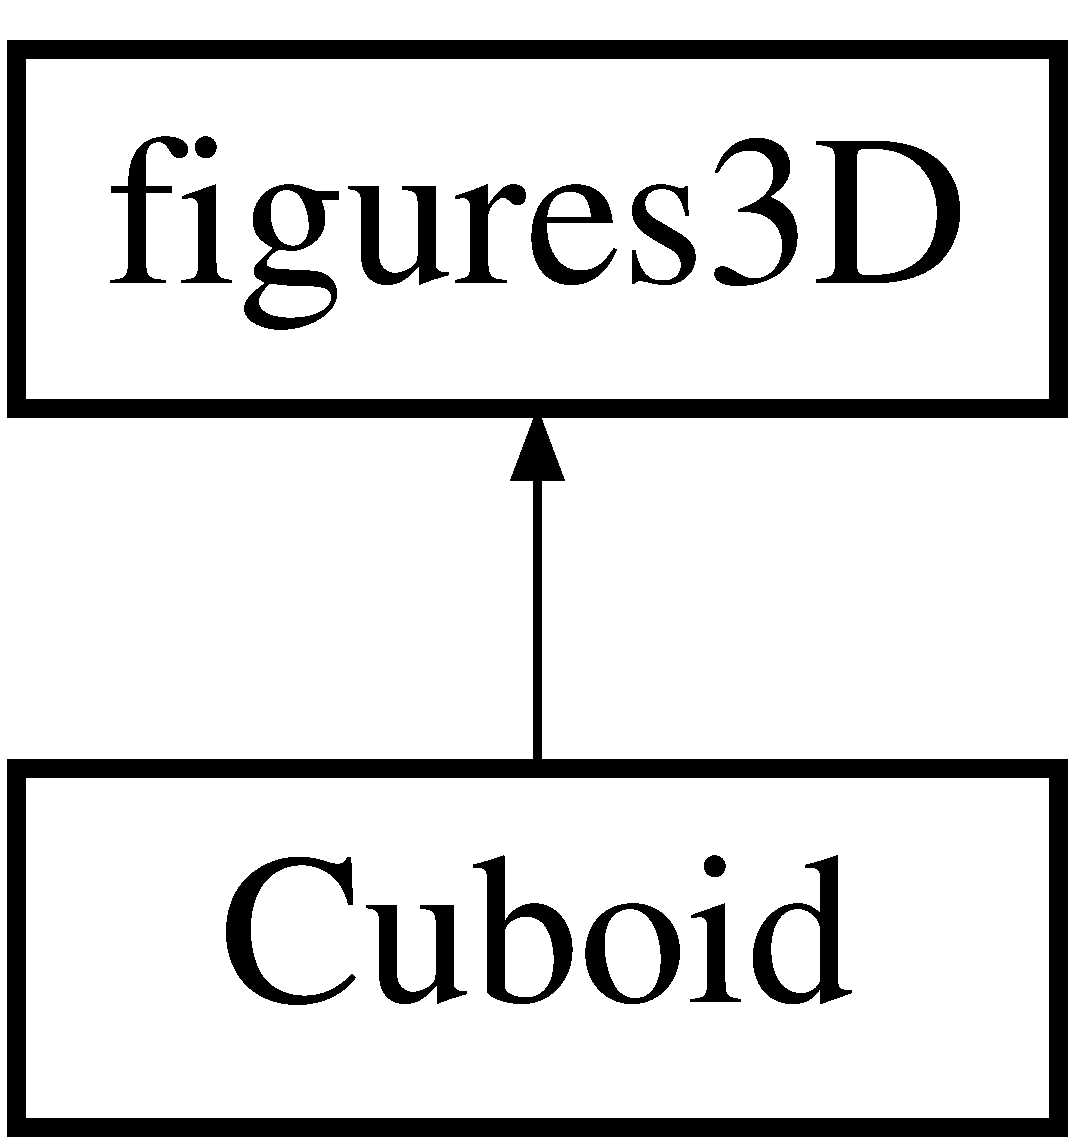
\includegraphics[height=2.000000cm]{class_cuboid}
\end{center}
\end{figure}
\subsection*{Public Member Functions}
\begin{DoxyCompactItemize}
\item 
\hyperlink{class_cuboid_a1abf60e93d024b7a01ee5b1a48f1f08a}{Cuboid} ()
\begin{DoxyCompactList}\small\item\em Tworzymy nowy obiekt prostopadloscianu. \end{DoxyCompactList}\item 
\hyperlink{class_cuboid_abd381a00b4e6fd8375b6c801a9380e18}{Cuboid} (double $\ast$change)
\begin{DoxyCompactList}\small\item\em Construct a new \hyperlink{class_cuboid}{Cuboid} object. \end{DoxyCompactList}\item 
\hyperlink{class_cuboid_aeecc4924bc1456780b20c3048e3515f9}{Cuboid} (\hyperlink{vector3_d_8hh_a8790ef07836c1639da216f46501979c0}{Vector3D} centre, \hyperlink{vector3_d_8hh_a8790ef07836c1639da216f46501979c0}{Vector3D} size)
\begin{DoxyCompactList}\small\item\em Construct a new \hyperlink{class_cuboid}{Cuboid} object. \end{DoxyCompactList}\item 
\hyperlink{vector3_d_8hh_a8790ef07836c1639da216f46501979c0}{Vector3D} \hyperlink{class_cuboid_a1bd1aaaa5b60441acf5d75c56a7f3b53}{Get\+Symetry\+Point} () const 
\begin{DoxyCompactList}\small\item\em Pozyskanie punktu symetrii prostopadloscianu. \end{DoxyCompactList}\end{DoxyCompactItemize}
\subsection*{Additional Inherited Members}


\subsection{Constructor \& Destructor Documentation}
\index{Cuboid@{Cuboid}!Cuboid@{Cuboid}}
\index{Cuboid@{Cuboid}!Cuboid@{Cuboid}}
\subsubsection[{\texorpdfstring{Cuboid()}{Cuboid()}}]{\setlength{\rightskip}{0pt plus 5cm}Cuboid\+::\+Cuboid (
\begin{DoxyParamCaption}
{}
\end{DoxyParamCaption}
)}\hypertarget{class_cuboid_a1abf60e93d024b7a01ee5b1a48f1f08a}{}\label{class_cuboid_a1abf60e93d024b7a01ee5b1a48f1f08a}
Automatycznie przypisujemy wierzcholki Dzieki temu uzytkownik nie musi podawac wierzcholkow, tylko operuje na gotowym obiekcie \index{Cuboid@{Cuboid}!Cuboid@{Cuboid}}
\index{Cuboid@{Cuboid}!Cuboid@{Cuboid}}
\subsubsection[{\texorpdfstring{Cuboid(double $\ast$change)}{Cuboid(double *change)}}]{\setlength{\rightskip}{0pt plus 5cm}Cuboid\+::\+Cuboid (
\begin{DoxyParamCaption}
\item[{double $\ast$}]{change}
\end{DoxyParamCaption}
)}\hypertarget{class_cuboid_abd381a00b4e6fd8375b6c801a9380e18}{}\label{class_cuboid_abd381a00b4e6fd8375b6c801a9380e18}

\begin{DoxyParams}{Parameters}
{\em change} & -\/ zestaw parametrow okreslajacyh ustawienia i rozmiar prostopadloscianu kolejno\+: x,y,z,scalex,scaley,scalez \\
\hline
\end{DoxyParams}
\index{Cuboid@{Cuboid}!Cuboid@{Cuboid}}
\index{Cuboid@{Cuboid}!Cuboid@{Cuboid}}
\subsubsection[{\texorpdfstring{Cuboid(\+Vector3\+D centre, Vector3\+D size)}{Cuboid(Vector3D centre, Vector3D size)}}]{\setlength{\rightskip}{0pt plus 5cm}Cuboid\+::\+Cuboid (
\begin{DoxyParamCaption}
\item[{{\bf Vector3D}}]{centre, }
\item[{{\bf Vector3D}}]{size}
\end{DoxyParamCaption}
)}\hypertarget{class_cuboid_aeecc4924bc1456780b20c3048e3515f9}{}\label{class_cuboid_aeecc4924bc1456780b20c3048e3515f9}

\begin{DoxyParams}{Parameters}
{\em centre} & -\/ srodek symetri nowego prostopadloscianu \\
\hline
{\em size} & -\/ rozmiary prostopadloscianu \\
\hline
\end{DoxyParams}


\subsection{Member Function Documentation}
\index{Cuboid@{Cuboid}!Get\+Symetry\+Point@{Get\+Symetry\+Point}}
\index{Get\+Symetry\+Point@{Get\+Symetry\+Point}!Cuboid@{Cuboid}}
\subsubsection[{\texorpdfstring{Get\+Symetry\+Point() const }{GetSymetryPoint() const }}]{\setlength{\rightskip}{0pt plus 5cm}{\bf Vector3D} Cuboid\+::\+Get\+Symetry\+Point (
\begin{DoxyParamCaption}
{}
\end{DoxyParamCaption}
) const}\hypertarget{class_cuboid_a1bd1aaaa5b60441acf5d75c56a7f3b53}{}\label{class_cuboid_a1bd1aaaa5b60441acf5d75c56a7f3b53}
Za punkt symetrii przyjeto srodek ciezkosci prostopadloscianu Funkcja to moze byc wykorzystywana do przesuwania wspolrzednych do ukladu wspolrzednych prosotpadloscianu

\begin{DoxyReturn}{Returns}
Vector3D -\/ punkt symetrii 
\end{DoxyReturn}


The documentation for this class was generated from the following files\+:\begin{DoxyCompactItemize}
\item 
\hyperlink{cuboid_8hh}{cuboid.\+hh}\item 
\hyperlink{cuboid_8cpp}{cuboid.\+cpp}\end{DoxyCompactItemize}

\hypertarget{classfigures3_d}{}\section{figures3D Class Reference}
\label{classfigures3_d}\index{figures3D@{figures3D}}


Model szerokiego pojecia figury geometrycznej 3-\/wymiarowej, klasy nadrzednej.  




{\ttfamily \#include $<$figures3\+D.\+hh$>$}

Inheritance diagram for figures3D\+:\begin{figure}[H]
\begin{center}
\leavevmode
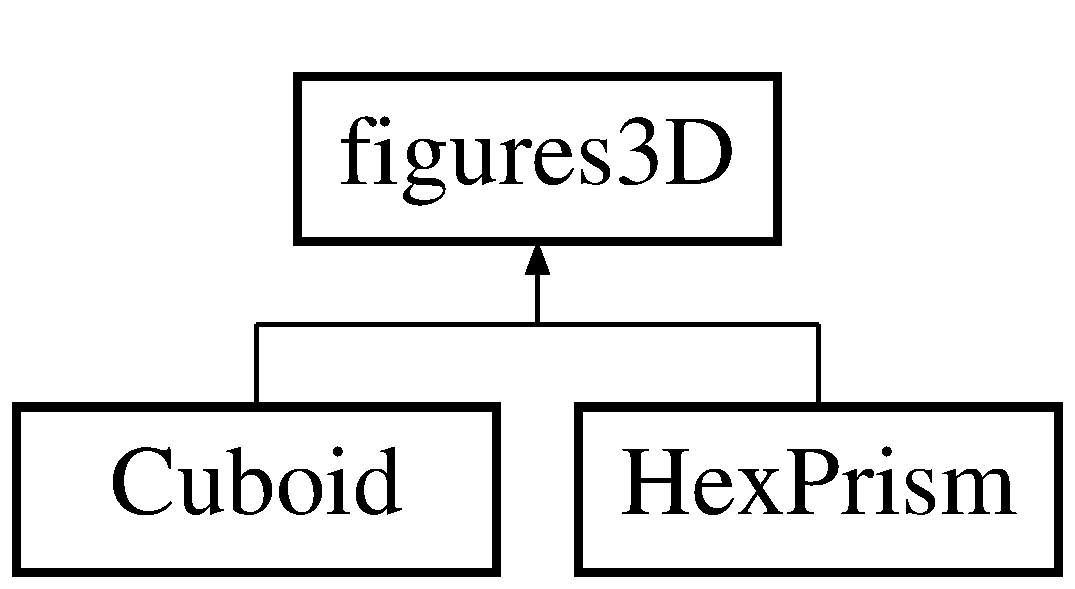
\includegraphics[height=2.000000cm]{classfigures3_d}
\end{center}
\end{figure}
\subsection*{Public Member Functions}
\begin{DoxyCompactItemize}
\item 
\hyperlink{vector3_d_8hh_a8790ef07836c1639da216f46501979c0}{Vector3D} \& \hyperlink{classfigures3_d_af35b8d1711f6fe2738af86d2641ce5aa}{operator\mbox{[}$\,$\mbox{]}} (int Index)
\begin{DoxyCompactList}\small\item\em Odwolanie do wierzcholka z mozliwa zmiana wartosci. \end{DoxyCompactList}\item 
\hyperlink{vector3_d_8hh_a8790ef07836c1639da216f46501979c0}{Vector3D} \hyperlink{classfigures3_d_adee2c4a6f78ee8deb5b57194ef3025d8}{operator\mbox{[}$\,$\mbox{]}} (int Index) const 
\begin{DoxyCompactList}\small\item\em Odowolanie do wierzcholka bez mozliwosci zmiany wartosci. \end{DoxyCompactList}\item 
void \hyperlink{classfigures3_d_a630645770668a4a1b35762a311db39b8}{rotate} (\hyperlink{matrix3x3_8hh_ae0d6db325717593a1d1157ecfa156f13}{Matrix3x3} matrix)
\begin{DoxyCompactList}\small\item\em Rotacja kazdego punktu nalezacego do figury. \end{DoxyCompactList}\item 
void \hyperlink{classfigures3_d_a6fddc70b227f21d8c32b0f741b536b05}{Translate} (\hyperlink{vector3_d_8hh_a8790ef07836c1639da216f46501979c0}{Vector3D} offset)
\begin{DoxyCompactList}\small\item\em translacja kazdego punktu nalezacego do danej figury \end{DoxyCompactList}\end{DoxyCompactItemize}
\subsection*{Protected Attributes}
\begin{DoxyCompactItemize}
\item 
vector$<$ \hyperlink{vector3_d_8hh_a8790ef07836c1639da216f46501979c0}{Vector3D} $>$ \hyperlink{classfigures3_d_a491e0281ce1e02aa7159840923cb3ef6}{P}
\begin{DoxyCompactList}\small\item\em wierzcholki figury geometrycznej lub punkty nalezace do niej, mozna stworzyc dowolna ilosc wierzcholkow \end{DoxyCompactList}\end{DoxyCompactItemize}


\subsection{Detailed Description}
Plik zawiera model pojecia figury geometrycznej 3-\/wymiarowej Zawiera typowe atrybuty i metody ktore moze posiadac dowolna figura geometryczna 

\subsection{Member Function Documentation}
\index{figures3D@{figures3D}!operator\mbox{[}$\,$\mbox{]}@{operator[]}}
\index{operator\mbox{[}$\,$\mbox{]}@{operator[]}!figures3D@{figures3D}}
\subsubsection[{\texorpdfstring{operator[](int Index)}{operator[](int Index)}}]{\setlength{\rightskip}{0pt plus 5cm}{\bf Vector3D}\& figures3\+D\+::operator\mbox{[}$\,$\mbox{]} (
\begin{DoxyParamCaption}
\item[{int}]{Index}
\end{DoxyParamCaption}
)\hspace{0.3cm}{\ttfamily [inline]}}\hypertarget{classfigures3_d_af35b8d1711f6fe2738af86d2641ce5aa}{}\label{classfigures3_d_af35b8d1711f6fe2738af86d2641ce5aa}

\begin{DoxyParams}{Parameters}
{\em Index} & -\/ indeks wierzcholka \\
\hline
\end{DoxyParams}
\begin{DoxyReturn}{Returns}
Vector3D\& -\/ zwracamy wierzcholek 
\end{DoxyReturn}
\index{figures3D@{figures3D}!operator\mbox{[}$\,$\mbox{]}@{operator[]}}
\index{operator\mbox{[}$\,$\mbox{]}@{operator[]}!figures3D@{figures3D}}
\subsubsection[{\texorpdfstring{operator[](int Index) const }{operator[](int Index) const }}]{\setlength{\rightskip}{0pt plus 5cm}{\bf Vector3D} figures3\+D\+::operator\mbox{[}$\,$\mbox{]} (
\begin{DoxyParamCaption}
\item[{int}]{Index}
\end{DoxyParamCaption}
) const\hspace{0.3cm}{\ttfamily [inline]}}\hypertarget{classfigures3_d_adee2c4a6f78ee8deb5b57194ef3025d8}{}\label{classfigures3_d_adee2c4a6f78ee8deb5b57194ef3025d8}

\begin{DoxyParams}{Parameters}
{\em Index} & -\/ indeks wierzcholka \\
\hline
\end{DoxyParams}
\begin{DoxyReturn}{Returns}
Vector3D -\/ zwracamy wierzcholek 
\end{DoxyReturn}
\index{figures3D@{figures3D}!rotate@{rotate}}
\index{rotate@{rotate}!figures3D@{figures3D}}
\subsubsection[{\texorpdfstring{rotate(\+Matrix3x3 matrix)}{rotate(Matrix3x3 matrix)}}]{\setlength{\rightskip}{0pt plus 5cm}void figures3\+D\+::rotate (
\begin{DoxyParamCaption}
\item[{{\bf Matrix3x3}}]{matrix}
\end{DoxyParamCaption}
)}\hypertarget{classfigures3_d_a630645770668a4a1b35762a311db39b8}{}\label{classfigures3_d_a630645770668a4a1b35762a311db39b8}

\begin{DoxyParams}{Parameters}
{\em matrix} & -\/ macierz obrotu \\
\hline
\end{DoxyParams}
\index{figures3D@{figures3D}!Translate@{Translate}}
\index{Translate@{Translate}!figures3D@{figures3D}}
\subsubsection[{\texorpdfstring{Translate(\+Vector3\+D offset)}{Translate(Vector3D offset)}}]{\setlength{\rightskip}{0pt plus 5cm}void figures3\+D\+::\+Translate (
\begin{DoxyParamCaption}
\item[{{\bf Vector3D}}]{offset}
\end{DoxyParamCaption}
)}\hypertarget{classfigures3_d_a6fddc70b227f21d8c32b0f741b536b05}{}\label{classfigures3_d_a6fddc70b227f21d8c32b0f741b536b05}

\begin{DoxyParams}{Parameters}
{\em offset} & -\/zadany wektor translacji \\
\hline
\end{DoxyParams}


\subsection{Member Data Documentation}
\index{figures3D@{figures3D}!P@{P}}
\index{P@{P}!figures3D@{figures3D}}
\subsubsection[{\texorpdfstring{P}{P}}]{\setlength{\rightskip}{0pt plus 5cm}vector$<${\bf Vector3D}$>$ figures3\+D\+::P\hspace{0.3cm}{\ttfamily [protected]}}\hypertarget{classfigures3_d_a491e0281ce1e02aa7159840923cb3ef6}{}\label{classfigures3_d_a491e0281ce1e02aa7159840923cb3ef6}


The documentation for this class was generated from the following files\+:\begin{DoxyCompactItemize}
\item 
\hyperlink{figures3_d_8hh}{figures3\+D.\+hh}\item 
\hyperlink{figures3_d_8cpp}{figures3\+D.\+cpp}\end{DoxyCompactItemize}

\hypertarget{class_pz_g_1_1_file_info}{}\section{PzG\+:\+:File\+Info Class Reference}
\label{class_pz_g_1_1_file_info}\index{Pz\+G\+::\+File\+Info@{Pz\+G\+::\+File\+Info}}


Zestaw informacji dotyczący pliku i sposobu rysowania.  




{\ttfamily \#include $<$gnuplot\+\_\+link.\+hh$>$}

\subsection*{Public Member Functions}
\begin{DoxyCompactItemize}
\item 
\hyperlink{class_pz_g_1_1_file_info_a09603738e0fbc8d6dadda905a5e947d7}{File\+Info} (std\+::string filename, \hyperlink{namespace_pz_g_ab0580cdb6bfe9e51d7de2588bc824076}{Line\+Style} style, int width)
\item 
const std\+::string \hyperlink{class_pz_g_1_1_file_info_a22aff3716073c3755d308851ce253188}{Get\+Filename} () const 
\begin{DoxyCompactList}\small\item\em Udostępia nazwę pliku do rysowania. \end{DoxyCompactList}\item 
void \hyperlink{class_pz_g_1_1_file_info_a02c728f892c6f169b738adac8ed9d5f1}{Set\+Filename} (const std\+::string \&filename)
\begin{DoxyCompactList}\small\item\em Zmienia nazwę pliku do rysowania. \end{DoxyCompactList}\item 
\hyperlink{namespace_pz_g_ab0580cdb6bfe9e51d7de2588bc824076}{Line\+Style} \hyperlink{class_pz_g_1_1_file_info_a9548e8dce5707b93edd5cc6d9fd06c0d}{Get\+Style} () const 
\begin{DoxyCompactList}\small\item\em Udostępnia sposób rysowanej linii. \end{DoxyCompactList}\item 
int \hyperlink{class_pz_g_1_1_file_info_a44863ad6997e427a736e8b4663d5a1bc}{Get\+Width} () const 
\begin{DoxyCompactList}\small\item\em Udostępnia informację o szerokości linii. \end{DoxyCompactList}\end{DoxyCompactItemize}
\subsection*{Private Attributes}
\begin{DoxyCompactItemize}
\item 
std\+::string \hyperlink{class_pz_g_1_1_file_info_a04f77a755e72bcf379844b15d9f0f3ed}{filename\+\_\+}
\begin{DoxyCompactList}\small\item\em Nazwa pliku z danymi do rysowania. \end{DoxyCompactList}\item 
int \hyperlink{class_pz_g_1_1_file_info_a1a1d3ea502a2604eec731ca50a2b438f}{width\+\_\+}
\begin{DoxyCompactList}\small\item\em Szerokość użytego piórka. \end{DoxyCompactList}\item 
\hyperlink{namespace_pz_g_ab0580cdb6bfe9e51d7de2588bc824076}{Line\+Style} \hyperlink{class_pz_g_1_1_file_info_a9141a03aee9840ebe103e4b1b6fa5c9b}{style\+\_\+}
\begin{DoxyCompactList}\small\item\em Sposób rysowania danej linii. \end{DoxyCompactList}\end{DoxyCompactItemize}


\subsection{Detailed Description}
Klasa modeluje zestaw informacji dotyczący pliku i sposobu w jaki mają być wizualizowane zawarte w nim dane. 

\subsection{Constructor \& Destructor Documentation}
\index{Pz\+G\+::\+File\+Info@{Pz\+G\+::\+File\+Info}!File\+Info@{File\+Info}}
\index{File\+Info@{File\+Info}!Pz\+G\+::\+File\+Info@{Pz\+G\+::\+File\+Info}}
\subsubsection[{\texorpdfstring{File\+Info(std\+::string filename, Line\+Style style, int width)}{FileInfo(std::string filename, LineStyle style, int width)}}]{\setlength{\rightskip}{0pt plus 5cm}Pz\+G\+::\+File\+Info\+::\+File\+Info (
\begin{DoxyParamCaption}
\item[{std\+::string}]{filename, }
\item[{{\bf Line\+Style}}]{style, }
\item[{int}]{width}
\end{DoxyParamCaption}
)\hspace{0.3cm}{\ttfamily [inline]}}\hypertarget{class_pz_g_1_1_file_info_a09603738e0fbc8d6dadda905a5e947d7}{}\label{class_pz_g_1_1_file_info_a09603738e0fbc8d6dadda905a5e947d7}
Inicjalizuje obiekt. 
\begin{DoxyParams}{Parameters}
{\em filename} & -\/ nazwa pliku, z którego pobierane będą dane, \\
\hline
{\em style} & -\/ rodzaj rysowania linii, \\
\hline
{\em width} & -\/ szerokosc linii. \\
\hline
\end{DoxyParams}


\subsection{Member Function Documentation}
\index{Pz\+G\+::\+File\+Info@{Pz\+G\+::\+File\+Info}!Get\+Filename@{Get\+Filename}}
\index{Get\+Filename@{Get\+Filename}!Pz\+G\+::\+File\+Info@{Pz\+G\+::\+File\+Info}}
\subsubsection[{\texorpdfstring{Get\+Filename() const }{GetFilename() const }}]{\setlength{\rightskip}{0pt plus 5cm}const std\+::string Pz\+G\+::\+File\+Info\+::\+Get\+Filename (
\begin{DoxyParamCaption}
{}
\end{DoxyParamCaption}
) const\hspace{0.3cm}{\ttfamily [inline]}}\hypertarget{class_pz_g_1_1_file_info_a22aff3716073c3755d308851ce253188}{}\label{class_pz_g_1_1_file_info_a22aff3716073c3755d308851ce253188}
Udostępnia nazwę pliku z danymi do rysowania. \index{Pz\+G\+::\+File\+Info@{Pz\+G\+::\+File\+Info}!Get\+Style@{Get\+Style}}
\index{Get\+Style@{Get\+Style}!Pz\+G\+::\+File\+Info@{Pz\+G\+::\+File\+Info}}
\subsubsection[{\texorpdfstring{Get\+Style() const }{GetStyle() const }}]{\setlength{\rightskip}{0pt plus 5cm}{\bf Line\+Style} Pz\+G\+::\+File\+Info\+::\+Get\+Style (
\begin{DoxyParamCaption}
{}
\end{DoxyParamCaption}
) const\hspace{0.3cm}{\ttfamily [inline]}}\hypertarget{class_pz_g_1_1_file_info_a9548e8dce5707b93edd5cc6d9fd06c0d}{}\label{class_pz_g_1_1_file_info_a9548e8dce5707b93edd5cc6d9fd06c0d}
Udostępnia informację o sposóbie rysowania linii. \index{Pz\+G\+::\+File\+Info@{Pz\+G\+::\+File\+Info}!Get\+Width@{Get\+Width}}
\index{Get\+Width@{Get\+Width}!Pz\+G\+::\+File\+Info@{Pz\+G\+::\+File\+Info}}
\subsubsection[{\texorpdfstring{Get\+Width() const }{GetWidth() const }}]{\setlength{\rightskip}{0pt plus 5cm}int Pz\+G\+::\+File\+Info\+::\+Get\+Width (
\begin{DoxyParamCaption}
{}
\end{DoxyParamCaption}
) const\hspace{0.3cm}{\ttfamily [inline]}}\hypertarget{class_pz_g_1_1_file_info_a44863ad6997e427a736e8b4663d5a1bc}{}\label{class_pz_g_1_1_file_info_a44863ad6997e427a736e8b4663d5a1bc}
Udostępnia informację o szerokości rysowanej linii. \index{Pz\+G\+::\+File\+Info@{Pz\+G\+::\+File\+Info}!Set\+Filename@{Set\+Filename}}
\index{Set\+Filename@{Set\+Filename}!Pz\+G\+::\+File\+Info@{Pz\+G\+::\+File\+Info}}
\subsubsection[{\texorpdfstring{Set\+Filename(const std\+::string \&filename)}{SetFilename(const std::string &filename)}}]{\setlength{\rightskip}{0pt plus 5cm}void Pz\+G\+::\+File\+Info\+::\+Set\+Filename (
\begin{DoxyParamCaption}
\item[{const std\+::string \&}]{filename}
\end{DoxyParamCaption}
)\hspace{0.3cm}{\ttfamily [inline]}}\hypertarget{class_pz_g_1_1_file_info_a02c728f892c6f169b738adac8ed9d5f1}{}\label{class_pz_g_1_1_file_info_a02c728f892c6f169b738adac8ed9d5f1}
Zmienia nazwę pliku z danymi do rysowania. 

\subsection{Member Data Documentation}
\index{Pz\+G\+::\+File\+Info@{Pz\+G\+::\+File\+Info}!filename\+\_\+@{filename\+\_\+}}
\index{filename\+\_\+@{filename\+\_\+}!Pz\+G\+::\+File\+Info@{Pz\+G\+::\+File\+Info}}
\subsubsection[{\texorpdfstring{filename\+\_\+}{filename_}}]{\setlength{\rightskip}{0pt plus 5cm}std\+::string Pz\+G\+::\+File\+Info\+::filename\+\_\+\hspace{0.3cm}{\ttfamily [private]}}\hypertarget{class_pz_g_1_1_file_info_a04f77a755e72bcf379844b15d9f0f3ed}{}\label{class_pz_g_1_1_file_info_a04f77a755e72bcf379844b15d9f0f3ed}
Nazwa pliku z danymi do rysowania. \index{Pz\+G\+::\+File\+Info@{Pz\+G\+::\+File\+Info}!style\+\_\+@{style\+\_\+}}
\index{style\+\_\+@{style\+\_\+}!Pz\+G\+::\+File\+Info@{Pz\+G\+::\+File\+Info}}
\subsubsection[{\texorpdfstring{style\+\_\+}{style_}}]{\setlength{\rightskip}{0pt plus 5cm}{\bf Line\+Style} Pz\+G\+::\+File\+Info\+::style\+\_\+\hspace{0.3cm}{\ttfamily [private]}}\hypertarget{class_pz_g_1_1_file_info_a9141a03aee9840ebe103e4b1b6fa5c9b}{}\label{class_pz_g_1_1_file_info_a9141a03aee9840ebe103e4b1b6fa5c9b}
Przechowuje informacje o sposobie rysowania linii. \index{Pz\+G\+::\+File\+Info@{Pz\+G\+::\+File\+Info}!width\+\_\+@{width\+\_\+}}
\index{width\+\_\+@{width\+\_\+}!Pz\+G\+::\+File\+Info@{Pz\+G\+::\+File\+Info}}
\subsubsection[{\texorpdfstring{width\+\_\+}{width_}}]{\setlength{\rightskip}{0pt plus 5cm}int Pz\+G\+::\+File\+Info\+::width\+\_\+\hspace{0.3cm}{\ttfamily [private]}}\hypertarget{class_pz_g_1_1_file_info_a1a1d3ea502a2604eec731ca50a2b438f}{}\label{class_pz_g_1_1_file_info_a1a1d3ea502a2604eec731ca50a2b438f}
Określa szerokość piórka, jakie ma być użyte do rysowania obiektów graficznych. 

The documentation for this class was generated from the following file\+:\begin{DoxyCompactItemize}
\item 
\hyperlink{gnuplot__link_8hh}{gnuplot\+\_\+link.\+hh}\end{DoxyCompactItemize}

\hypertarget{class_pz_g_1_1_gnuplot_link}{}\section{PzG\+:\+:Gnuplot\+Link Class Reference}
\label{class_pz_g_1_1_gnuplot_link}\index{Pz\+G\+::\+Gnuplot\+Link@{Pz\+G\+::\+Gnuplot\+Link}}


Klasa realizuje interfejs do programu G\+N\+U\+Plot.  




{\ttfamily \#include $<$gnuplot\+\_\+link.\+hh$>$}

\subsection*{Public Member Functions}
\begin{DoxyCompactItemize}
\item 
void \hyperlink{class_pz_g_1_1_gnuplot_link_abd99d3a72eebe5c6323be5cf4a465b34}{show\+\_\+\+O\+X\+\_\+axis} (bool show)
\begin{DoxyCompactList}\small\item\em Umożliwia lub zabrania rysowania osi OX. \end{DoxyCompactList}\item 
bool \hyperlink{class_pz_g_1_1_gnuplot_link_a94cb61a141da389031bdaa2fd1a2f9d0}{show\+\_\+\+O\+X\+\_\+axis} () const 
\begin{DoxyCompactList}\small\item\em Czy oś OX ma być rysowana. \end{DoxyCompactList}\item 
void \hyperlink{class_pz_g_1_1_gnuplot_link_a345cd5f032c34ffcc1e3aa16438dda82}{show\+\_\+\+O\+Y\+\_\+axis} (bool show)
\begin{DoxyCompactList}\small\item\em Umożliwia lub zabrania rysowania osi OY. \end{DoxyCompactList}\item 
bool \hyperlink{class_pz_g_1_1_gnuplot_link_a7221ba30e2c2d736c9b314a0ad751823}{show\+\_\+\+O\+Y\+\_\+axis} () const 
\begin{DoxyCompactList}\small\item\em Czy oś OY ma być rysowana. \end{DoxyCompactList}\item 
void \hyperlink{class_pz_g_1_1_gnuplot_link_ab4e8078f7c63779d5f4c21f22608d3ef}{show\+\_\+\+O\+Z\+\_\+axis} (bool show)
\begin{DoxyCompactList}\small\item\em Umożliwia lub zabrania rysowania osi OZ. \end{DoxyCompactList}\item 
bool \hyperlink{class_pz_g_1_1_gnuplot_link_ab64b940900a005045dce0f4a13f2ab54}{show\+\_\+\+O\+Z\+\_\+axis} () const 
\begin{DoxyCompactList}\small\item\em Czy oś OZ ma być rysowana. \end{DoxyCompactList}\item 
float \hyperlink{class_pz_g_1_1_gnuplot_link_afb8a3cb4ceb164a81bc49a5f15da712c}{Xmin} () const 
\item 
float \hyperlink{class_pz_g_1_1_gnuplot_link_a3a52abbe4b555f7e021f11d7af4950e8}{Xmax} () const 
\item 
float \hyperlink{class_pz_g_1_1_gnuplot_link_a88ccb047ebb0d79fa008e8347c57d742}{Ymin} () const 
\item 
float \hyperlink{class_pz_g_1_1_gnuplot_link_a438a7d313d30a209ef413aa1c339bb1e}{Ymax} () const 
\item 
float \hyperlink{class_pz_g_1_1_gnuplot_link_a5bc2e5f8c07dbe7d0f4e3f3ec3475769}{Zmin} () const 
\item 
float \hyperlink{class_pz_g_1_1_gnuplot_link_ad69c4841d707b9a19b003a46d6f80460}{Zmax} () const 
\item 
void \hyperlink{class_pz_g_1_1_gnuplot_link_a5b903bc69eb4c2884edbe25d53cea188}{Set\+Drawing\+Mode} (\hyperlink{namespace_pz_g_a4360c76a1dbf714a19a0d97fe56e0660}{Drawing\+Mode} mode)
\begin{DoxyCompactList}\small\item\em Zmienia tryb rysowania. \end{DoxyCompactList}\item 
\hyperlink{namespace_pz_g_a4360c76a1dbf714a19a0d97fe56e0660}{Drawing\+Mode} \hyperlink{class_pz_g_1_1_gnuplot_link_a04f53a5fa365789ea6a4fa2142b686dc}{Get\+Drawing\+Mode} () const 
\begin{DoxyCompactList}\small\item\em Udostępnia aktualny tryb rysowania. \end{DoxyCompactList}\item 
void \hyperlink{class_pz_g_1_1_gnuplot_link_a7db1d889cd30bfb23cb4af3ca4bb4ef0}{Set\+RangeX} (float Xo, float Xn)
\begin{DoxyCompactList}\small\item\em Ustawia zakres osi {\itshape OX}. \end{DoxyCompactList}\item 
void \hyperlink{class_pz_g_1_1_gnuplot_link_a269f721e7d49c37a842c1f65511a7d71}{Set\+RangeY} (float Yo, float Yn)
\begin{DoxyCompactList}\small\item\em Ustawia zakres osi {\itshape OY}. \end{DoxyCompactList}\item 
void \hyperlink{class_pz_g_1_1_gnuplot_link_a6cb4123fb2cbe459a747c2a1c1f94770}{Set\+RangeZ} (float Zo, float Zn)
\begin{DoxyCompactList}\small\item\em Ustawia zakres osi {\itshape OZ}. \end{DoxyCompactList}\item 
float \hyperlink{class_pz_g_1_1_gnuplot_link_a60f11dbb42e3f8704572b1837236ee3f}{ScaleX} () const 
\begin{DoxyCompactList}\small\item\em Udostępnia skalę dla osi {\itshape OX}. \end{DoxyCompactList}\item 
float \hyperlink{class_pz_g_1_1_gnuplot_link_ab8a72e0e53ef198cba596f6c895b30cf}{ScaleZ} () const 
\begin{DoxyCompactList}\small\item\em Udostępnia skalę dla osi {\itshape OZ}. \end{DoxyCompactList}\item 
void \hyperlink{class_pz_g_1_1_gnuplot_link_a70d30fdb78dad112f96963a55f69e279}{Set\+ScaleX} (float x\+\_\+scale)
\begin{DoxyCompactList}\small\item\em Zadaje skalę wzdłuż osi {\itshape OZ}. \end{DoxyCompactList}\item 
void \hyperlink{class_pz_g_1_1_gnuplot_link_adb266ff0cb6bc916dcb12b6bd168ba14}{Set\+ScaleZ} (float z\+\_\+scale)
\begin{DoxyCompactList}\small\item\em Zadaje skalę wzdłuż osi {\itshape OZ}. \end{DoxyCompactList}\item 
void \hyperlink{class_pz_g_1_1_gnuplot_link_a922cef9903317477051890311f6f4dec}{Set\+Scale\+XZ} (float x\+\_\+scale, float z\+\_\+scale)
\begin{DoxyCompactList}\small\item\em Zadaje skalę wzdłuż osi {\itshape OX} i {\itshape OZ}. \end{DoxyCompactList}\item 
float \hyperlink{class_pz_g_1_1_gnuplot_link_a5af6158903c5defc05e96318af4ff8ce}{RotationX} () const 
\item 
float \hyperlink{class_pz_g_1_1_gnuplot_link_ac7601ea2c0af006013790b325781fb7c}{RotationZ} () const 
\item 
void \hyperlink{class_pz_g_1_1_gnuplot_link_ace414a178fc745111344ce2390e363b7}{Set\+RotationX} (float x\+\_\+angle)
\begin{DoxyCompactList}\small\item\em Ustawia rotację wokół osi {\itshape OX}. \end{DoxyCompactList}\item 
void \hyperlink{class_pz_g_1_1_gnuplot_link_a2d72e30d46e7fb61fbf70f2ea5c0d0a5}{Set\+RotationZ} (float z\+\_\+angle)
\begin{DoxyCompactList}\small\item\em Ustawia rotację wokół osi {\itshape OZ}. \end{DoxyCompactList}\item 
void \hyperlink{class_pz_g_1_1_gnuplot_link_ae1019984feb2a9cef9c8b41eec65ee97}{Set\+Rotation\+XZ} (float x\+\_\+angle, float z\+\_\+angle)
\begin{DoxyCompactList}\small\item\em Ustawia rotację wokół osi {\itshape OX} i {\itshape OZ}. \end{DoxyCompactList}\item 
void \hyperlink{class_pz_g_1_1_gnuplot_link_a9c8f23498ce784bd4f62583163e9c065}{Show\+Error\+Messages} (bool mode=true)
\begin{DoxyCompactList}\small\item\em Zezwala lub zabrania wyświetlania komunikatów. \end{DoxyCompactList}\item 
bool \hyperlink{class_pz_g_1_1_gnuplot_link_a795ee974694d79694496e09d668eb562}{Add\+Filename} (const char $\ast$filename, \hyperlink{namespace_pz_g_ab0580cdb6bfe9e51d7de2588bc824076}{Line\+Style} style=\hyperlink{namespace_pz_g_ab0580cdb6bfe9e51d7de2588bc824076af8f97c84dadf8eaa1f0370861e15dfec}{L\+S\+\_\+\+C\+O\+N\+T\+I\+N\+U\+O\+US}, int width=1)
\begin{DoxyCompactList}\small\item\em Dodaje nazwę pliku. \end{DoxyCompactList}\item 
bool \hyperlink{class_pz_g_1_1_gnuplot_link_a8f6eb81e4b1324d338a13de9fe692583}{Add\+Drawing\+From\+Files} (std\+::string \&command, char const $\ast$$\ast$separator)
\begin{DoxyCompactList}\small\item\em Tworzy listę parametrów umożliwiających rysowanie brył z plików. \end{DoxyCompactList}\item 
bool \hyperlink{class_pz_g_1_1_gnuplot_link_a515a61833bc59ed29e7fafab3ca93918}{Is\+Connection\+Initialized} () const 
\begin{DoxyCompactList}\small\item\em Informuje, czy połączenie z {\itshape gnuplot\textquotesingle{}em} jest zainicjalizowane. \end{DoxyCompactList}\item 
bool \hyperlink{class_pz_g_1_1_gnuplot_link_a96321ba10f7ee9c5f55dd17a28143a39}{Draw} ()
\item 
bool \hyperlink{class_pz_g_1_1_gnuplot_link_a77b3776f569733b570681190b12d1891}{Draw\+To\+File} (const char $\ast$filename)
\item 
bool \hyperlink{class_pz_g_1_1_gnuplot_link_a7f9c65c2319f35f1b7663ba0ad461d14}{Init} ()
\begin{DoxyCompactList}\small\item\em Inicjalizuje połączenie z programem {\itshape gnuplot}. \end{DoxyCompactList}\item 
void \hyperlink{class_pz_g_1_1_gnuplot_link_acd96e1e3a99df66cfd68971f9974661f}{Delete\+Last\+Name} ()
\begin{DoxyCompactList}\small\item\em Usuwa ostatnią nazwę pliku. \end{DoxyCompactList}\item 
void \hyperlink{class_pz_g_1_1_gnuplot_link_aa0e5912cf21d3e4ebaedfc4d473f1008}{Delete\+All\+Names} ()
\begin{DoxyCompactList}\small\item\em Kasuje zawartość listy nazw plików. \end{DoxyCompactList}\item 
\hyperlink{class_pz_g_1_1_gnuplot_link_aa140852169cf67df9c565c33a45bff75}{Gnuplot\+Link} ()
\item 
virtual \hyperlink{class_pz_g_1_1_gnuplot_link_adba8f71e0828a077757dae54918c0b45}{$\sim$\+Gnuplot\+Link} ()
\end{DoxyCompactItemize}
\subsection*{Protected Member Functions}
\begin{DoxyCompactItemize}
\item 
virtual bool \hyperlink{class_pz_g_1_1_gnuplot_link_a0e0854467fcaf528a04a32e1e4e3fa37}{Add\+Files\+To\+Draw\+Command} (std\+::string \&command, char const $\ast$$\ast$separator)
\begin{DoxyCompactList}\small\item\em Tworzy listę parametrów umożliwiających rysowanie dodatkowych elementów. \end{DoxyCompactList}\item 
std\+::string \hyperlink{class_pz_g_1_1_gnuplot_link_a5b7fdc2909ad007b5915fe30439fbb9e}{Save\+Range\+Settings} (char axis) const 
\begin{DoxyCompactList}\small\item\em Tworzy polecenie ustawiające zakres dla danej współrzędnej. \end{DoxyCompactList}\item 
std\+::string \hyperlink{class_pz_g_1_1_gnuplot_link_aa95135aad76f86efd1d60518abacbeb4}{Save\+Scale\+Rotation\+Settings} () const 
\begin{DoxyCompactList}\small\item\em Tworzy polecenie ustawiające punkt obserwacji. \end{DoxyCompactList}\item 
bool \hyperlink{class_pz_g_1_1_gnuplot_link_acf0c0bf937eb87f9c14dedf2f01780bc}{Send\+To\+Gnuplot} (const char $\ast$command)
\item 
bool \hyperlink{class_pz_g_1_1_gnuplot_link_a65e94fe30d1d5f4b369fecb344e4629f}{Are\+Error\+Messages\+Displayed} () const 
\begin{DoxyCompactList}\small\item\em Udostępnia informację czy mają być wyświetlane informacje o błędach. \end{DoxyCompactList}\item 
bool \hyperlink{class_pz_g_1_1_gnuplot_link_a81a78898b39cb0b4c79ea4f3c90bbeb5}{Create\+Child\+Process} ()
\begin{DoxyCompactList}\small\item\em Uruchamia program {\itshape gnuplot} jako proces potomny. \end{DoxyCompactList}\item 
void \hyperlink{class_pz_g_1_1_gnuplot_link_af16d87b0f93073a69b921668790884f4}{Error\+Message} (const char $\ast$message) const 
\item 
void \hyperlink{class_pz_g_1_1_gnuplot_link_a1d9ac939f5871ca51d283422327906ba}{Create\+Command\+Preamble} (std\+::string \&preamble) const 
\begin{DoxyCompactList}\small\item\em Tworzy preambułę poprzedzającą polecenie rysowania. \end{DoxyCompactList}\item 
void \hyperlink{class_pz_g_1_1_gnuplot_link_a540eea1303ac48055d88a57a0f7dda8f}{Create2\+D\+Preamble} (std\+::string \&preamble) const 
\begin{DoxyCompactList}\small\item\em Tworzy preambułę poprzedzającą polecenie rysowania w trybie 2D. \end{DoxyCompactList}\item 
void \hyperlink{class_pz_g_1_1_gnuplot_link_a0cfefccf9eaf44292417834525053dab}{Create3\+D\+Preamble} (std\+::string \&preamble) const 
\begin{DoxyCompactList}\small\item\em Tworzy preambułę poprzedzającą polecenie rysowania w trybie 3D. \end{DoxyCompactList}\end{DoxyCompactItemize}
\subsection*{Protected Attributes}
\begin{DoxyCompactItemize}
\item 
int \hyperlink{class_pz_g_1_1_gnuplot_link_a8b04a557aacb13f62a46bd0cd1233119}{gnuplot\+\_\+input\+\_\+}
\item 
int \hyperlink{class_pz_g_1_1_gnuplot_link_a3ba099cef3e84aab2d3d0f7e99661cca}{gnuplot\+\_\+output\+\_\+}
\item 
bool \hyperlink{class_pz_g_1_1_gnuplot_link_adefdb7c360e54c586b1d6bd1fa5c6eee}{display\+\_\+error\+\_\+messages\+\_\+}
\begin{DoxyCompactList}\small\item\em Decyduje czy mają być wyświetlane komunikaty o błędach, czy też nie. \end{DoxyCompactList}\item 
\hyperlink{namespace_pz_g_a4360c76a1dbf714a19a0d97fe56e0660}{Drawing\+Mode} \hyperlink{class_pz_g_1_1_gnuplot_link_afe3cae0470049aee3c7350f488a630b6}{drawing\+\_\+mode\+\_\+}
\begin{DoxyCompactList}\small\item\em Określa aktualny tryb rysowania. \end{DoxyCompactList}\item 
float \hyperlink{class_pz_g_1_1_gnuplot_link_a9ca081e311914fb07ee4c292b8090247}{x\+\_\+min\+\_\+}
\begin{DoxyCompactList}\small\item\em Dolny zakres wyświetlanej skali skali dla osi {\itshape OX}. \end{DoxyCompactList}\item 
float \hyperlink{class_pz_g_1_1_gnuplot_link_a1f8870f0cc643c5ef931b30b40b5e282}{x\+\_\+max\+\_\+}
\begin{DoxyCompactList}\small\item\em Górny zakres wyświetlanej skali skali dla osi {\itshape OX}. \end{DoxyCompactList}\item 
float \hyperlink{class_pz_g_1_1_gnuplot_link_a31c8d2fcb350d54d09134c0f0a838aea}{y\+\_\+min\+\_\+}
\begin{DoxyCompactList}\small\item\em Dolny zakres wyświetlanej skali skali dla osi {\itshape OY}. \end{DoxyCompactList}\item 
float \hyperlink{class_pz_g_1_1_gnuplot_link_a9fb5609ee05da82c3a5c9f94416c1ac1}{y\+\_\+max\+\_\+}
\begin{DoxyCompactList}\small\item\em Górny zakres wyświetlanej skali skali dla osi {\itshape OY}. \end{DoxyCompactList}\item 
float \hyperlink{class_pz_g_1_1_gnuplot_link_a3a92421a06513241d150ec36eedcfb70}{z\+\_\+min\+\_\+}
\begin{DoxyCompactList}\small\item\em Dolny zakres wyświetlanej skali skali dla osi {\itshape OZ}. \end{DoxyCompactList}\item 
float \hyperlink{class_pz_g_1_1_gnuplot_link_ad16243c88647f80c0f69a6d04021dbf7}{z\+\_\+max\+\_\+}
\begin{DoxyCompactList}\small\item\em Górny zakres wyświetlanej skali skali dla osi {\itshape OZ}. \end{DoxyCompactList}\item 
float \hyperlink{class_pz_g_1_1_gnuplot_link_a725cf4ed098148a0e9b10ed94023757a}{x\+\_\+scale\+\_\+}
\item 
float \hyperlink{class_pz_g_1_1_gnuplot_link_a9926edcec6c7080a35f62c050f2773dc}{z\+\_\+scale\+\_\+}
\item 
float \hyperlink{class_pz_g_1_1_gnuplot_link_ae105dcd466bbc10f0b70ed753e0c2e4e}{x\+\_\+rotation\+\_\+}
\item 
float \hyperlink{class_pz_g_1_1_gnuplot_link_ae7ae9a0985b545d636908deb232f716c}{z\+\_\+rotation\+\_\+}
\item 
bool \hyperlink{class_pz_g_1_1_gnuplot_link_a694fd1200f95c4e8c1fcb0bfe30ab711}{show\+\_\+\+O\+X\+\_\+axis\+\_\+}
\begin{DoxyCompactList}\small\item\em Czy oś OX ma być widoczna. \end{DoxyCompactList}\item 
bool \hyperlink{class_pz_g_1_1_gnuplot_link_a6e6dbfa4c5d4ee81ef83afc1b4ad1be4}{show\+\_\+\+O\+Y\+\_\+axis\+\_\+}
\begin{DoxyCompactList}\small\item\em Czy oś OY ma być widoczna. \end{DoxyCompactList}\item 
bool \hyperlink{class_pz_g_1_1_gnuplot_link_a436e59363f312d5a98548526ced023ca}{show\+\_\+\+O\+Z\+\_\+axis\+\_\+}
\begin{DoxyCompactList}\small\item\em Czy oś OZ ma być widoczna. \end{DoxyCompactList}\end{DoxyCompactItemize}
\subsection*{Static Protected Attributes}
\begin{DoxyCompactItemize}
\item 
static std\+::list$<$ \hyperlink{class_pz_g_1_1_file_info}{File\+Info} $>$ \hyperlink{class_pz_g_1_1_gnuplot_link_af4b03524d7d1ccb3f09524217048ef5d}{files\+\_\+information\+\_\+}
\begin{DoxyCompactList}\small\item\em Lista nazw plików z danymi dla {\itshape gnuplota}. \end{DoxyCompactList}\end{DoxyCompactItemize}


\subsection{Detailed Description}
Klasa realizuje interfejs do programu G\+N\+U\+Plot. Pozwala ona na wskazanie zbioru punktów płaszczyzn umieszczonych w pliku lub plikach. Każdy taki zbiór może być następnie wizualizowany przez program gnuplot w postaci oddzielnych płaszczyzn z wycinaniem części zasłanianych. 

\subsection{Constructor \& Destructor Documentation}
\index{Pz\+G\+::\+Gnuplot\+Link@{Pz\+G\+::\+Gnuplot\+Link}!Gnuplot\+Link@{Gnuplot\+Link}}
\index{Gnuplot\+Link@{Gnuplot\+Link}!Pz\+G\+::\+Gnuplot\+Link@{Pz\+G\+::\+Gnuplot\+Link}}
\subsubsection[{\texorpdfstring{Gnuplot\+Link()}{GnuplotLink()}}]{\setlength{\rightskip}{0pt plus 5cm}Pz\+G\+::\+Gnuplot\+Link\+::\+Gnuplot\+Link (
\begin{DoxyParamCaption}
{}
\end{DoxyParamCaption}
)}\hypertarget{class_pz_g_1_1_gnuplot_link_aa140852169cf67df9c565c33a45bff75}{}\label{class_pz_g_1_1_gnuplot_link_aa140852169cf67df9c565c33a45bff75}
\index{Pz\+G\+::\+Gnuplot\+Link@{Pz\+G\+::\+Gnuplot\+Link}!````~Gnuplot\+Link@{$\sim$\+Gnuplot\+Link}}
\index{````~Gnuplot\+Link@{$\sim$\+Gnuplot\+Link}!Pz\+G\+::\+Gnuplot\+Link@{Pz\+G\+::\+Gnuplot\+Link}}
\subsubsection[{\texorpdfstring{$\sim$\+Gnuplot\+Link()}{~GnuplotLink()}}]{\setlength{\rightskip}{0pt plus 5cm}Pz\+G\+::\+Gnuplot\+Link\+::$\sim$\+Gnuplot\+Link (
\begin{DoxyParamCaption}
{}
\end{DoxyParamCaption}
)\hspace{0.3cm}{\ttfamily [virtual]}}\hypertarget{class_pz_g_1_1_gnuplot_link_adba8f71e0828a077757dae54918c0b45}{}\label{class_pz_g_1_1_gnuplot_link_adba8f71e0828a077757dae54918c0b45}


\subsection{Member Function Documentation}
\index{Pz\+G\+::\+Gnuplot\+Link@{Pz\+G\+::\+Gnuplot\+Link}!Add\+Drawing\+From\+Files@{Add\+Drawing\+From\+Files}}
\index{Add\+Drawing\+From\+Files@{Add\+Drawing\+From\+Files}!Pz\+G\+::\+Gnuplot\+Link@{Pz\+G\+::\+Gnuplot\+Link}}
\subsubsection[{\texorpdfstring{Add\+Drawing\+From\+Files(std\+::string \&command, char const $\ast$$\ast$separator)}{AddDrawingFromFiles(std::string &command, char const **separator)}}]{\setlength{\rightskip}{0pt plus 5cm}bool Pz\+G\+::\+Gnuplot\+Link\+::\+Add\+Drawing\+From\+Files (
\begin{DoxyParamCaption}
\item[{std\+::string \&}]{command, }
\item[{char const $\ast$$\ast$}]{separator}
\end{DoxyParamCaption}
)}\hypertarget{class_pz_g_1_1_gnuplot_link_a8f6eb81e4b1324d338a13de9fe692583}{}\label{class_pz_g_1_1_gnuplot_link_a8f6eb81e4b1324d338a13de9fe692583}
Tworzy napis będący parametrami dla polecenie {\itshape plot} programu, {\itshape gnuplot}. Parametry te pozwalają na rysowanie brył, których współrzędne wierzchołków zawarte są w plikach. Nazwy tych plików muszą być wcześniej dołączone do kolejki plików poprzez zastosowanie polecenia \hyperlink{}{Dodaj\+Nazwe}.


\begin{DoxyParams}{Parameters}
{\em command} & -\/ dopisywana jest do niego sekwencja znaków tworzących parametry dla polecenia {\itshape plot}. \\
\hline
{\em separator} & -\/ zawiera znak separatora między poszczególnymi parametrami. Jeżeli parametry listy nazw plików są generowane jako pierwsze, to zmienna ta musi być wskaźnikiem do wskaźnika na łańcuch\+: \char`\"{} \char`\"{}. \\
\hline
\end{DoxyParams}

\begin{DoxyRetVals}{Return values}
{\em true} & -\/ jeśli lista nazw plików nie jest pusta. \\
\hline
{\em false} & -\/ w przypadku przeciwnym. \\
\hline
\end{DoxyRetVals}
\begin{DoxyPostcond}{Postcondition}
Jeżeli lista nazw plików nie jest pusta, to poprzez parametr {\itshape separator} zostaje udostępniony łańcuch\+: \char`\"{}, \char`\"{}. 
\end{DoxyPostcond}
\index{Pz\+G\+::\+Gnuplot\+Link@{Pz\+G\+::\+Gnuplot\+Link}!Add\+Filename@{Add\+Filename}}
\index{Add\+Filename@{Add\+Filename}!Pz\+G\+::\+Gnuplot\+Link@{Pz\+G\+::\+Gnuplot\+Link}}
\subsubsection[{\texorpdfstring{Add\+Filename(const char $\ast$filename, Line\+Style style=\+L\+S\+\_\+\+C\+O\+N\+T\+I\+N\+U\+O\+U\+S, int width=1)}{AddFilename(const char *filename, LineStyle style=LS_CONTINUOUS, int width=1)}}]{\setlength{\rightskip}{0pt plus 5cm}bool Pz\+G\+::\+Gnuplot\+Link\+::\+Add\+Filename (
\begin{DoxyParamCaption}
\item[{const char $\ast$}]{filename, }
\item[{{\bf Line\+Style}}]{style = {\ttfamily {\bf L\+S\+\_\+\+C\+O\+N\+T\+I\+N\+U\+O\+US}}, }
\item[{int}]{width = {\ttfamily 1}}
\end{DoxyParamCaption}
)}\hypertarget{class_pz_g_1_1_gnuplot_link_a795ee974694d79694496e09d668eb562}{}\label{class_pz_g_1_1_gnuplot_link_a795ee974694d79694496e09d668eb562}
Powoduje dodanie do listy plików zawierajacych dane dla {\itshape gnuplota}, nowej nazwy pliku.


\begin{DoxyParams}[1]{Parameters}
\mbox{\tt in}  & {\em filename} & -\/ nazwa pliku z danymi dla gnuplota. \\
\hline
\mbox{\tt in}  & {\em style} & -\/ tryb rysowania danego zbioru punktow. Może być ciągły lub jako zbiór osobnych punktów. \\
\hline
\mbox{\tt in}  & {\em width} & -\/ szerokość rysowanego obiektu. W przypadku punktów parametr ten jest połową szerokości kwadratu reprezentującego dany punkt.\\
\hline
\end{DoxyParams}

\begin{DoxyRetVals}{Return values}
{\em true} & -\/ jeżeli istnieje plik o nazwie udostępnionej poprzez parametr {\itshape filename} oraz jest zezwolenie na jego czytanie. Nazwa pliku zostaje dodana do listy plików z danymi dla {\itshape gnuplota}. \\
\hline
{\em false} & -\/ Jeżeli nie istnieje plik o nazwie przekazanej poprzez parametr {\itshape filename}. Nazwa pliku zostaje dodana do listy plików z danymi dla {\itshape gnuplota}. \\
\hline
\end{DoxyRetVals}
\index{Pz\+G\+::\+Gnuplot\+Link@{Pz\+G\+::\+Gnuplot\+Link}!Add\+Files\+To\+Draw\+Command@{Add\+Files\+To\+Draw\+Command}}
\index{Add\+Files\+To\+Draw\+Command@{Add\+Files\+To\+Draw\+Command}!Pz\+G\+::\+Gnuplot\+Link@{Pz\+G\+::\+Gnuplot\+Link}}
\subsubsection[{\texorpdfstring{Add\+Files\+To\+Draw\+Command(std\+::string \&command, char const $\ast$$\ast$separator)}{AddFilesToDrawCommand(std::string &command, char const **separator)}}]{\setlength{\rightskip}{0pt plus 5cm}bool Pz\+G\+::\+Gnuplot\+Link\+::\+Add\+Files\+To\+Draw\+Command (
\begin{DoxyParamCaption}
\item[{std\+::string \&}]{command, }
\item[{char const $\ast$$\ast$}]{separator}
\end{DoxyParamCaption}
)\hspace{0.3cm}{\ttfamily [inline]}, {\ttfamily [protected]}, {\ttfamily [virtual]}}\hypertarget{class_pz_g_1_1_gnuplot_link_a0e0854467fcaf528a04a32e1e4e3fa37}{}\label{class_pz_g_1_1_gnuplot_link_a0e0854467fcaf528a04a32e1e4e3fa37}
Metoda ta przewidziana jest jako element rozszerzenia pozwalającego w klasach pochodnych powiększyć listę rysowanych elementów. \begin{DoxyPrecond}{Precondition}
Parametr {\itshape command} powinien zawierać polecenie {\itshape plot} lub {\itshape splot}, do którego będzie możliwe dopisanie dalszego ciągu. 
\end{DoxyPrecond}

\begin{DoxyParams}{Parameters}
{\em command} & -\/ polecenie rysowania, do którego mają być dopisane nazwy plików i odpowiednie parametry dla polecenia plot. \\
\hline
{\em separator} & -\/ zawiera znak separatora między poszczególnymi parametrami. Jeżeli parametry listy przeszkód są generowane jako pierwsze, to zmienna ta musi być wskaźnikiem do wskaźnika na łańcuch\+: \char`\"{} \char`\"{}. \\
\hline
\end{DoxyParams}
\index{Pz\+G\+::\+Gnuplot\+Link@{Pz\+G\+::\+Gnuplot\+Link}!Are\+Error\+Messages\+Displayed@{Are\+Error\+Messages\+Displayed}}
\index{Are\+Error\+Messages\+Displayed@{Are\+Error\+Messages\+Displayed}!Pz\+G\+::\+Gnuplot\+Link@{Pz\+G\+::\+Gnuplot\+Link}}
\subsubsection[{\texorpdfstring{Are\+Error\+Messages\+Displayed() const }{AreErrorMessagesDisplayed() const }}]{\setlength{\rightskip}{0pt plus 5cm}bool Pz\+G\+::\+Gnuplot\+Link\+::\+Are\+Error\+Messages\+Displayed (
\begin{DoxyParamCaption}
{}
\end{DoxyParamCaption}
) const\hspace{0.3cm}{\ttfamily [inline]}, {\ttfamily [protected]}}\hypertarget{class_pz_g_1_1_gnuplot_link_a65e94fe30d1d5f4b369fecb344e4629f}{}\label{class_pz_g_1_1_gnuplot_link_a65e94fe30d1d5f4b369fecb344e4629f}
Udostępnia wartość pola \hyperlink{class_pz_g_1_1_gnuplot_link_adefdb7c360e54c586b1d6bd1fa5c6eee}{display\+\_\+error\+\_\+messages\+\_\+}. Określa ono, czy mają być wyświetlane komunikaty o błędach na wyjście standardowe, czy też nie. \index{Pz\+G\+::\+Gnuplot\+Link@{Pz\+G\+::\+Gnuplot\+Link}!Create2\+D\+Preamble@{Create2\+D\+Preamble}}
\index{Create2\+D\+Preamble@{Create2\+D\+Preamble}!Pz\+G\+::\+Gnuplot\+Link@{Pz\+G\+::\+Gnuplot\+Link}}
\subsubsection[{\texorpdfstring{Create2\+D\+Preamble(std\+::string \&preamble) const }{Create2DPreamble(std::string &preamble) const }}]{\setlength{\rightskip}{0pt plus 5cm}void Pz\+G\+::\+Gnuplot\+Link\+::\+Create2\+D\+Preamble (
\begin{DoxyParamCaption}
\item[{std\+::string \&}]{preamble}
\end{DoxyParamCaption}
) const\hspace{0.3cm}{\ttfamily [protected]}}\hypertarget{class_pz_g_1_1_gnuplot_link_a540eea1303ac48055d88a57a0f7dda8f}{}\label{class_pz_g_1_1_gnuplot_link_a540eea1303ac48055d88a57a0f7dda8f}
Tworzy zbiór poleceń, które ustawiają właściwy tryb rysowania oraz zakresy współrzędnych, jak też wszystkie inne parametry wynikające z trybu rysowania 2D. \index{Pz\+G\+::\+Gnuplot\+Link@{Pz\+G\+::\+Gnuplot\+Link}!Create3\+D\+Preamble@{Create3\+D\+Preamble}}
\index{Create3\+D\+Preamble@{Create3\+D\+Preamble}!Pz\+G\+::\+Gnuplot\+Link@{Pz\+G\+::\+Gnuplot\+Link}}
\subsubsection[{\texorpdfstring{Create3\+D\+Preamble(std\+::string \&preamble) const }{Create3DPreamble(std::string &preamble) const }}]{\setlength{\rightskip}{0pt plus 5cm}void Pz\+G\+::\+Gnuplot\+Link\+::\+Create3\+D\+Preamble (
\begin{DoxyParamCaption}
\item[{std\+::string \&}]{preamble}
\end{DoxyParamCaption}
) const\hspace{0.3cm}{\ttfamily [protected]}}\hypertarget{class_pz_g_1_1_gnuplot_link_a0cfefccf9eaf44292417834525053dab}{}\label{class_pz_g_1_1_gnuplot_link_a0cfefccf9eaf44292417834525053dab}
Tworzy zbiór poleceń, które ustawiają właściwy tryb rysowania oraz zakresy współrzędnych, jak też wszystkie inne parametry wynikające z trybu rysowania 3D. \index{Pz\+G\+::\+Gnuplot\+Link@{Pz\+G\+::\+Gnuplot\+Link}!Create\+Child\+Process@{Create\+Child\+Process}}
\index{Create\+Child\+Process@{Create\+Child\+Process}!Pz\+G\+::\+Gnuplot\+Link@{Pz\+G\+::\+Gnuplot\+Link}}
\subsubsection[{\texorpdfstring{Create\+Child\+Process()}{CreateChildProcess()}}]{\setlength{\rightskip}{0pt plus 5cm}bool Pz\+G\+::\+Gnuplot\+Link\+::\+Create\+Child\+Process (
\begin{DoxyParamCaption}
{}
\end{DoxyParamCaption}
)\hspace{0.3cm}{\ttfamily [protected]}}\hypertarget{class_pz_g_1_1_gnuplot_link_a81a78898b39cb0b4c79ea4f3c90bbeb5}{}\label{class_pz_g_1_1_gnuplot_link_a81a78898b39cb0b4c79ea4f3c90bbeb5}
Inicjalizuje połączenie z programem {\itshape gnuplot}. Realizowane jest to poprzez rozwidlenie procesu i uruchomienie jako procesu potomnego programu {\itshape gnuplot}. Komunikacja z programem {\itshape gnuplot} realizowana jest poprzez przejęcie jego wejścia i wyjścia standardowego.


\begin{DoxyRetVals}{Return values}
{\em true} & -\/ gdy połączenie z programem {\itshape gnuplot} zostało poprawnie zainicjalizowane lub gdy już wcześniej było zainicjalizowane. \\
\hline
{\em false} & -\/ gdy proces inicjalizacji połączenia zakończył się niepowodzeniem. \\
\hline
\end{DoxyRetVals}
\index{Pz\+G\+::\+Gnuplot\+Link@{Pz\+G\+::\+Gnuplot\+Link}!Create\+Command\+Preamble@{Create\+Command\+Preamble}}
\index{Create\+Command\+Preamble@{Create\+Command\+Preamble}!Pz\+G\+::\+Gnuplot\+Link@{Pz\+G\+::\+Gnuplot\+Link}}
\subsubsection[{\texorpdfstring{Create\+Command\+Preamble(std\+::string \&preamble) const }{CreateCommandPreamble(std::string &preamble) const }}]{\setlength{\rightskip}{0pt plus 5cm}void Pz\+G\+::\+Gnuplot\+Link\+::\+Create\+Command\+Preamble (
\begin{DoxyParamCaption}
\item[{std\+::string \&}]{preamble}
\end{DoxyParamCaption}
) const\hspace{0.3cm}{\ttfamily [protected]}}\hypertarget{class_pz_g_1_1_gnuplot_link_a1d9ac939f5871ca51d283422327906ba}{}\label{class_pz_g_1_1_gnuplot_link_a1d9ac939f5871ca51d283422327906ba}
Tworzy zbiór poleceń, które ustawiają właściwy tryb rysowania oraz zakresy współrzędnych, jak też wszystkie inne parametry wynikające z przyjętego trybu rysowania. \index{Pz\+G\+::\+Gnuplot\+Link@{Pz\+G\+::\+Gnuplot\+Link}!Delete\+All\+Names@{Delete\+All\+Names}}
\index{Delete\+All\+Names@{Delete\+All\+Names}!Pz\+G\+::\+Gnuplot\+Link@{Pz\+G\+::\+Gnuplot\+Link}}
\subsubsection[{\texorpdfstring{Delete\+All\+Names()}{DeleteAllNames()}}]{\setlength{\rightskip}{0pt plus 5cm}void Pz\+G\+::\+Gnuplot\+Link\+::\+Delete\+All\+Names (
\begin{DoxyParamCaption}
{}
\end{DoxyParamCaption}
)}\hypertarget{class_pz_g_1_1_gnuplot_link_aa0e5912cf21d3e4ebaedfc4d473f1008}{}\label{class_pz_g_1_1_gnuplot_link_aa0e5912cf21d3e4ebaedfc4d473f1008}
Calkowicie kasuje zawartość listy nazw plików. \index{Pz\+G\+::\+Gnuplot\+Link@{Pz\+G\+::\+Gnuplot\+Link}!Delete\+Last\+Name@{Delete\+Last\+Name}}
\index{Delete\+Last\+Name@{Delete\+Last\+Name}!Pz\+G\+::\+Gnuplot\+Link@{Pz\+G\+::\+Gnuplot\+Link}}
\subsubsection[{\texorpdfstring{Delete\+Last\+Name()}{DeleteLastName()}}]{\setlength{\rightskip}{0pt plus 5cm}void Pz\+G\+::\+Gnuplot\+Link\+::\+Delete\+Last\+Name (
\begin{DoxyParamCaption}
{}
\end{DoxyParamCaption}
)}\hypertarget{class_pz_g_1_1_gnuplot_link_acd96e1e3a99df66cfd68971f9974661f}{}\label{class_pz_g_1_1_gnuplot_link_acd96e1e3a99df66cfd68971f9974661f}
Usuwa ostatnią nazwę z listy nazw plików. \index{Pz\+G\+::\+Gnuplot\+Link@{Pz\+G\+::\+Gnuplot\+Link}!Draw@{Draw}}
\index{Draw@{Draw}!Pz\+G\+::\+Gnuplot\+Link@{Pz\+G\+::\+Gnuplot\+Link}}
\subsubsection[{\texorpdfstring{Draw()}{Draw()}}]{\setlength{\rightskip}{0pt plus 5cm}bool Pz\+G\+::\+Gnuplot\+Link\+::\+Draw (
\begin{DoxyParamCaption}
{}
\end{DoxyParamCaption}
)}\hypertarget{class_pz_g_1_1_gnuplot_link_a96321ba10f7ee9c5f55dd17a28143a39}{}\label{class_pz_g_1_1_gnuplot_link_a96321ba10f7ee9c5f55dd17a28143a39}
Jeżeli lista plików nie jest pusta, to generuje sekwencje poleceń dla programu {\itshape gnuplot} mająca na celu narysowanie płaszczyzn na na podstawie danych zawartych w plikach z listy.

\begin{DoxyPrecond}{Precondition}
Lista plików nie powinna być pusta. Nazwy plików na niej można umieścić za pomoca metody \hyperlink{}{Add\+Name}. Metoda nie wymaga wcześniejszego zainicjowania połączenia z {\itshape gnuplotem}. 
\end{DoxyPrecond}

\begin{DoxyRetVals}{Return values}
{\em true} & -\/ gdy zostają poprawnie wysłane polecenia dla gnuplota. Nie oznacza to jednak, że proces rysowania zakończył się pomyślnie. \\
\hline
{\em false} & -\/ gdy połączenie z gnuplotem nie może zostać poprawnie zainicjalizowane lub gdy lista plików jest pusta. \\
\hline
\end{DoxyRetVals}
\index{Pz\+G\+::\+Gnuplot\+Link@{Pz\+G\+::\+Gnuplot\+Link}!Draw\+To\+File@{Draw\+To\+File}}
\index{Draw\+To\+File@{Draw\+To\+File}!Pz\+G\+::\+Gnuplot\+Link@{Pz\+G\+::\+Gnuplot\+Link}}
\subsubsection[{\texorpdfstring{Draw\+To\+File(const char $\ast$filename)}{DrawToFile(const char *filename)}}]{\setlength{\rightskip}{0pt plus 5cm}bool Pz\+G\+::\+Gnuplot\+Link\+::\+Draw\+To\+File (
\begin{DoxyParamCaption}
\item[{const char $\ast$}]{filename}
\end{DoxyParamCaption}
)}\hypertarget{class_pz_g_1_1_gnuplot_link_a77b3776f569733b570681190b12d1891}{}\label{class_pz_g_1_1_gnuplot_link_a77b3776f569733b570681190b12d1891}
Działa analogicznie jak metoda \hyperlink{class_pz_g_1_1_gnuplot_link_a96321ba10f7ee9c5f55dd17a28143a39}{Draw}, z tą różnicą, że rysunek robota składowany jest w pliku o nazwie przekazanej przez parametr {\itshape filename}. Rysunek jest zapisywany w formacie {\itshape P\+NG}.

\begin{DoxyPostcond}{Postcondition}
Lista plików nie powinna być pusta ponadto powinno być możliwe otwarcie do zapisu pliku o nazwie przekazanej przez parametr {\itshape filename}, do której dołączane jest rozszerzenie .ps . Metoda nie wymaga wcześniejszego zainicjowania połączenia z programem {\itshape gnuplot}.
\end{DoxyPostcond}

\begin{DoxyRetVals}{Return values}
{\em true} & -\/ gdy zostają poprawnie wysłane polecenia dla {\itshape gnuplota}. Nie oznacza to jednak, że proces rysowania zakończył się pomyślnie. \\
\hline
{\em false} & -\/ gdy połączenie z gnuplotem nie może zostać poprawnie zainicjalizowane lub gdy lista plików jest pusta lub też gdy nie można otworzyć pliku do zapisu. \\
\hline
\end{DoxyRetVals}
\index{Pz\+G\+::\+Gnuplot\+Link@{Pz\+G\+::\+Gnuplot\+Link}!Error\+Message@{Error\+Message}}
\index{Error\+Message@{Error\+Message}!Pz\+G\+::\+Gnuplot\+Link@{Pz\+G\+::\+Gnuplot\+Link}}
\subsubsection[{\texorpdfstring{Error\+Message(const char $\ast$message) const }{ErrorMessage(const char *message) const }}]{\setlength{\rightskip}{0pt plus 5cm}void Pz\+G\+::\+Gnuplot\+Link\+::\+Error\+Message (
\begin{DoxyParamCaption}
\item[{const char $\ast$}]{message}
\end{DoxyParamCaption}
) const\hspace{0.3cm}{\ttfamily [protected]}}\hypertarget{class_pz_g_1_1_gnuplot_link_af16d87b0f93073a69b921668790884f4}{}\label{class_pz_g_1_1_gnuplot_link_af16d87b0f93073a69b921668790884f4}
Wyświetla na wyjście \char`\"{}standard error\char`\"{} komunikat (przekazany jako parametr), o ile pole \hyperlink{class_pz_g_1_1_gnuplot_link_adefdb7c360e54c586b1d6bd1fa5c6eee}{display\+\_\+error\+\_\+messages\+\_\+} ma wartość {\ttfamily true}. W przypadku przeciwnym komunikat nie jest wyświetlany. \index{Pz\+G\+::\+Gnuplot\+Link@{Pz\+G\+::\+Gnuplot\+Link}!Get\+Drawing\+Mode@{Get\+Drawing\+Mode}}
\index{Get\+Drawing\+Mode@{Get\+Drawing\+Mode}!Pz\+G\+::\+Gnuplot\+Link@{Pz\+G\+::\+Gnuplot\+Link}}
\subsubsection[{\texorpdfstring{Get\+Drawing\+Mode() const }{GetDrawingMode() const }}]{\setlength{\rightskip}{0pt plus 5cm}{\bf Drawing\+Mode} Pz\+G\+::\+Gnuplot\+Link\+::\+Get\+Drawing\+Mode (
\begin{DoxyParamCaption}
{}
\end{DoxyParamCaption}
) const\hspace{0.3cm}{\ttfamily [inline]}}\hypertarget{class_pz_g_1_1_gnuplot_link_a04f53a5fa365789ea6a4fa2142b686dc}{}\label{class_pz_g_1_1_gnuplot_link_a04f53a5fa365789ea6a4fa2142b686dc}
Udostępnia informację o aktualnym trybie rysowania. \index{Pz\+G\+::\+Gnuplot\+Link@{Pz\+G\+::\+Gnuplot\+Link}!Init@{Init}}
\index{Init@{Init}!Pz\+G\+::\+Gnuplot\+Link@{Pz\+G\+::\+Gnuplot\+Link}}
\subsubsection[{\texorpdfstring{Init()}{Init()}}]{\setlength{\rightskip}{0pt plus 5cm}bool Pz\+G\+::\+Gnuplot\+Link\+::\+Init (
\begin{DoxyParamCaption}
{}
\end{DoxyParamCaption}
)}\hypertarget{class_pz_g_1_1_gnuplot_link_a7f9c65c2319f35f1b7663ba0ad461d14}{}\label{class_pz_g_1_1_gnuplot_link_a7f9c65c2319f35f1b7663ba0ad461d14}
Inicjalizuje połączenie z programem {\itshape gnuplot}. Realizowane jest to poprzez rozwidlenie procesu i uruchomienie jako procesu potomnego programu {\itshape gnuplot}. Komunikacja z programem {\itshape gnuplot} realizowana jest poprzez przejęcie jego wejścia i wyjścia standardowego.


\begin{DoxyRetVals}{Return values}
{\em true} & -\/ gdy połączenie z programem {\itshape 0gnuplot} zostało poprawnie zainicjalizowane lub gdy już wcześniej było zainicjalizowane. \\
\hline
{\em false} & -\/ gdy proces inicjalizacji połączenia zakończył się niepowodzeniem. \\
\hline
\end{DoxyRetVals}
\index{Pz\+G\+::\+Gnuplot\+Link@{Pz\+G\+::\+Gnuplot\+Link}!Is\+Connection\+Initialized@{Is\+Connection\+Initialized}}
\index{Is\+Connection\+Initialized@{Is\+Connection\+Initialized}!Pz\+G\+::\+Gnuplot\+Link@{Pz\+G\+::\+Gnuplot\+Link}}
\subsubsection[{\texorpdfstring{Is\+Connection\+Initialized() const }{IsConnectionInitialized() const }}]{\setlength{\rightskip}{0pt plus 5cm}bool Pz\+G\+::\+Gnuplot\+Link\+::\+Is\+Connection\+Initialized (
\begin{DoxyParamCaption}
{}
\end{DoxyParamCaption}
) const}\hypertarget{class_pz_g_1_1_gnuplot_link_a515a61833bc59ed29e7fafab3ca93918}{}\label{class_pz_g_1_1_gnuplot_link_a515a61833bc59ed29e7fafab3ca93918}
Informuje, czy połączenie z programem {\itshape gnuplot} jest zainicjowane. 
\begin{DoxyRetVals}{Return values}
{\em true} & -\/ jeśli tak, \\
\hline
{\em false} & -\/ w przypadku przeciwnym. \\
\hline
\end{DoxyRetVals}
\index{Pz\+G\+::\+Gnuplot\+Link@{Pz\+G\+::\+Gnuplot\+Link}!RotationX@{RotationX}}
\index{RotationX@{RotationX}!Pz\+G\+::\+Gnuplot\+Link@{Pz\+G\+::\+Gnuplot\+Link}}
\subsubsection[{\texorpdfstring{Rotation\+X() const }{RotationX() const }}]{\setlength{\rightskip}{0pt plus 5cm}float Pz\+G\+::\+Gnuplot\+Link\+::\+RotationX (
\begin{DoxyParamCaption}
{}
\end{DoxyParamCaption}
) const\hspace{0.3cm}{\ttfamily [inline]}}\hypertarget{class_pz_g_1_1_gnuplot_link_a5af6158903c5defc05e96318af4ff8ce}{}\label{class_pz_g_1_1_gnuplot_link_a5af6158903c5defc05e96318af4ff8ce}
Udostępnia wartość kąta rotacji renderowanego rysunku wokół osi {\itshape OX}. Zwracana wartość wyrażona jest w stopiniach. \index{Pz\+G\+::\+Gnuplot\+Link@{Pz\+G\+::\+Gnuplot\+Link}!RotationZ@{RotationZ}}
\index{RotationZ@{RotationZ}!Pz\+G\+::\+Gnuplot\+Link@{Pz\+G\+::\+Gnuplot\+Link}}
\subsubsection[{\texorpdfstring{Rotation\+Z() const }{RotationZ() const }}]{\setlength{\rightskip}{0pt plus 5cm}float Pz\+G\+::\+Gnuplot\+Link\+::\+RotationZ (
\begin{DoxyParamCaption}
{}
\end{DoxyParamCaption}
) const\hspace{0.3cm}{\ttfamily [inline]}}\hypertarget{class_pz_g_1_1_gnuplot_link_ac7601ea2c0af006013790b325781fb7c}{}\label{class_pz_g_1_1_gnuplot_link_ac7601ea2c0af006013790b325781fb7c}
Udostępnia wartość kąta rotacji renderowanego rysunku wokół osi {\itshape OZ}. Zwracana wartość wyrażona jest w stopiniach. \index{Pz\+G\+::\+Gnuplot\+Link@{Pz\+G\+::\+Gnuplot\+Link}!Save\+Range\+Settings@{Save\+Range\+Settings}}
\index{Save\+Range\+Settings@{Save\+Range\+Settings}!Pz\+G\+::\+Gnuplot\+Link@{Pz\+G\+::\+Gnuplot\+Link}}
\subsubsection[{\texorpdfstring{Save\+Range\+Settings(char axis) const }{SaveRangeSettings(char axis) const }}]{\setlength{\rightskip}{0pt plus 5cm}std\+::string Pz\+G\+::\+Gnuplot\+Link\+::\+Save\+Range\+Settings (
\begin{DoxyParamCaption}
\item[{char}]{axis}
\end{DoxyParamCaption}
) const\hspace{0.3cm}{\ttfamily [protected]}}\hypertarget{class_pz_g_1_1_gnuplot_link_a5b7fdc2909ad007b5915fe30439fbb9e}{}\label{class_pz_g_1_1_gnuplot_link_a5b7fdc2909ad007b5915fe30439fbb9e}
Tworzy polecenie dla programu {\itshape gnuplot} ustawiające zakres współrzędnych wybranej współrzędnej {\itshape x}, {\itshape y} lub {\itshape z}, dla której ma być tworzony dany rysunek. 
\begin{DoxyParams}{Parameters}
{\em axis} & -\/ zawiera znak określający współrzędną, dla której ma zostać wygenerowane polecenie ustawienia zakresu. \\
\hline
\end{DoxyParams}
\begin{DoxyReturn}{Returns}
łańcuch znaków polecenia ustawiającego żądany zakres dla wybranej współrzędnej. 
\end{DoxyReturn}
\index{Pz\+G\+::\+Gnuplot\+Link@{Pz\+G\+::\+Gnuplot\+Link}!Save\+Scale\+Rotation\+Settings@{Save\+Scale\+Rotation\+Settings}}
\index{Save\+Scale\+Rotation\+Settings@{Save\+Scale\+Rotation\+Settings}!Pz\+G\+::\+Gnuplot\+Link@{Pz\+G\+::\+Gnuplot\+Link}}
\subsubsection[{\texorpdfstring{Save\+Scale\+Rotation\+Settings() const }{SaveScaleRotationSettings() const }}]{\setlength{\rightskip}{0pt plus 5cm}std\+::string Pz\+G\+::\+Gnuplot\+Link\+::\+Save\+Scale\+Rotation\+Settings (
\begin{DoxyParamCaption}
{}
\end{DoxyParamCaption}
) const\hspace{0.3cm}{\ttfamily [protected]}}\hypertarget{class_pz_g_1_1_gnuplot_link_aa95135aad76f86efd1d60518abacbeb4}{}\label{class_pz_g_1_1_gnuplot_link_aa95135aad76f86efd1d60518abacbeb4}
Tworzy polecenie dla programu {\itshape gnuplot} ustawiajające punkt obserwacji poprzez zadanie rotacji i skali dla poszczególnych osi. \index{Pz\+G\+::\+Gnuplot\+Link@{Pz\+G\+::\+Gnuplot\+Link}!ScaleX@{ScaleX}}
\index{ScaleX@{ScaleX}!Pz\+G\+::\+Gnuplot\+Link@{Pz\+G\+::\+Gnuplot\+Link}}
\subsubsection[{\texorpdfstring{Scale\+X() const }{ScaleX() const }}]{\setlength{\rightskip}{0pt plus 5cm}float Pz\+G\+::\+Gnuplot\+Link\+::\+ScaleX (
\begin{DoxyParamCaption}
{}
\end{DoxyParamCaption}
) const\hspace{0.3cm}{\ttfamily [inline]}}\hypertarget{class_pz_g_1_1_gnuplot_link_a60f11dbb42e3f8704572b1837236ee3f}{}\label{class_pz_g_1_1_gnuplot_link_a60f11dbb42e3f8704572b1837236ee3f}
Udostępnia skalę dla osi {\itshape OX} dla tworzonego rysunku. \index{Pz\+G\+::\+Gnuplot\+Link@{Pz\+G\+::\+Gnuplot\+Link}!ScaleZ@{ScaleZ}}
\index{ScaleZ@{ScaleZ}!Pz\+G\+::\+Gnuplot\+Link@{Pz\+G\+::\+Gnuplot\+Link}}
\subsubsection[{\texorpdfstring{Scale\+Z() const }{ScaleZ() const }}]{\setlength{\rightskip}{0pt plus 5cm}float Pz\+G\+::\+Gnuplot\+Link\+::\+ScaleZ (
\begin{DoxyParamCaption}
{}
\end{DoxyParamCaption}
) const\hspace{0.3cm}{\ttfamily [inline]}}\hypertarget{class_pz_g_1_1_gnuplot_link_ab8a72e0e53ef198cba596f6c895b30cf}{}\label{class_pz_g_1_1_gnuplot_link_ab8a72e0e53ef198cba596f6c895b30cf}
Udostępnia skalę dla osi {\itshape OZ} dla tworzonego rysunku. \index{Pz\+G\+::\+Gnuplot\+Link@{Pz\+G\+::\+Gnuplot\+Link}!Send\+To\+Gnuplot@{Send\+To\+Gnuplot}}
\index{Send\+To\+Gnuplot@{Send\+To\+Gnuplot}!Pz\+G\+::\+Gnuplot\+Link@{Pz\+G\+::\+Gnuplot\+Link}}
\subsubsection[{\texorpdfstring{Send\+To\+Gnuplot(const char $\ast$command)}{SendToGnuplot(const char *command)}}]{\setlength{\rightskip}{0pt plus 5cm}bool Pz\+G\+::\+Gnuplot\+Link\+::\+Send\+To\+Gnuplot (
\begin{DoxyParamCaption}
\item[{const char $\ast$}]{command}
\end{DoxyParamCaption}
)\hspace{0.3cm}{\ttfamily [protected]}}\hypertarget{class_pz_g_1_1_gnuplot_link_acf0c0bf937eb87f9c14dedf2f01780bc}{}\label{class_pz_g_1_1_gnuplot_link_acf0c0bf937eb87f9c14dedf2f01780bc}
Przesyła na wejście programu {\itshape gnuplot} zadany ciąg znaków. 
\begin{DoxyParams}{Parameters}
{\em command} & -\/ komunikat przeznaczony do przeslania.\\
\hline
\end{DoxyParams}
\begin{DoxyPrecond}{Precondition}
Musi być zainicjowane połączenie z programem gnuplot.
\end{DoxyPrecond}

\begin{DoxyRetVals}{Return values}
{\em true} & -\/ jesli przeslanie polecenia zakończyło się powodzeniem, \\
\hline
{\em false} & -\/ w przypadku przeciwnym. \\
\hline
\end{DoxyRetVals}
\index{Pz\+G\+::\+Gnuplot\+Link@{Pz\+G\+::\+Gnuplot\+Link}!Set\+Drawing\+Mode@{Set\+Drawing\+Mode}}
\index{Set\+Drawing\+Mode@{Set\+Drawing\+Mode}!Pz\+G\+::\+Gnuplot\+Link@{Pz\+G\+::\+Gnuplot\+Link}}
\subsubsection[{\texorpdfstring{Set\+Drawing\+Mode(\+Drawing\+Mode mode)}{SetDrawingMode(DrawingMode mode)}}]{\setlength{\rightskip}{0pt plus 5cm}void Pz\+G\+::\+Gnuplot\+Link\+::\+Set\+Drawing\+Mode (
\begin{DoxyParamCaption}
\item[{{\bf Drawing\+Mode}}]{mode}
\end{DoxyParamCaption}
)\hspace{0.3cm}{\ttfamily [inline]}}\hypertarget{class_pz_g_1_1_gnuplot_link_a5b903bc69eb4c2884edbe25d53cea188}{}\label{class_pz_g_1_1_gnuplot_link_a5b903bc69eb4c2884edbe25d53cea188}
Zmienia tryb rysowania jaki zostanie wymuszony na programie {\ttfamily gnuplot}. 
\begin{DoxyParams}{Parameters}
{\em mode} & -\/ wartość parametru określa nowy tryb rysowania. \\
\hline
\end{DoxyParams}
\index{Pz\+G\+::\+Gnuplot\+Link@{Pz\+G\+::\+Gnuplot\+Link}!Set\+RangeX@{Set\+RangeX}}
\index{Set\+RangeX@{Set\+RangeX}!Pz\+G\+::\+Gnuplot\+Link@{Pz\+G\+::\+Gnuplot\+Link}}
\subsubsection[{\texorpdfstring{Set\+Range\+X(float Xo, float Xn)}{SetRangeX(float Xo, float Xn)}}]{\setlength{\rightskip}{0pt plus 5cm}void Pz\+G\+::\+Gnuplot\+Link\+::\+Set\+RangeX (
\begin{DoxyParamCaption}
\item[{float}]{Xo, }
\item[{float}]{Xn}
\end{DoxyParamCaption}
)\hspace{0.3cm}{\ttfamily [inline]}}\hypertarget{class_pz_g_1_1_gnuplot_link_a7db1d889cd30bfb23cb4af3ca4bb4ef0}{}\label{class_pz_g_1_1_gnuplot_link_a7db1d889cd30bfb23cb4af3ca4bb4ef0}
Ustawia zakres osi {\itshape OX}. Ogranicza to obszar, który będzie zwizualizowany przez programa {\itshape gnuplot}. 
\begin{DoxyParams}{Parameters}
{\em Xo} & -\/ dolna granica obszaru rysowania dla osi {\itshape OX}. \\
\hline
{\em Xn} & -\/ górna granica obszaru rysowania dla osi {\itshape OX}. \\
\hline
\end{DoxyParams}
\index{Pz\+G\+::\+Gnuplot\+Link@{Pz\+G\+::\+Gnuplot\+Link}!Set\+RangeY@{Set\+RangeY}}
\index{Set\+RangeY@{Set\+RangeY}!Pz\+G\+::\+Gnuplot\+Link@{Pz\+G\+::\+Gnuplot\+Link}}
\subsubsection[{\texorpdfstring{Set\+Range\+Y(float Yo, float Yn)}{SetRangeY(float Yo, float Yn)}}]{\setlength{\rightskip}{0pt plus 5cm}void Pz\+G\+::\+Gnuplot\+Link\+::\+Set\+RangeY (
\begin{DoxyParamCaption}
\item[{float}]{Yo, }
\item[{float}]{Yn}
\end{DoxyParamCaption}
)\hspace{0.3cm}{\ttfamily [inline]}}\hypertarget{class_pz_g_1_1_gnuplot_link_a269f721e7d49c37a842c1f65511a7d71}{}\label{class_pz_g_1_1_gnuplot_link_a269f721e7d49c37a842c1f65511a7d71}
Ustawia zakres osi {\itshape OY}. Ogranicza to obszar, który będzie zwizualizowany przez programa {\itshape gnuplot}. 
\begin{DoxyParams}{Parameters}
{\em Yo} & -\/ dolna granica obszaru rysowania dla osi {\itshape OY}. \\
\hline
{\em Yn} & -\/ górna granica obszaru rysowania dla osi {\itshape OY}. \\
\hline
\end{DoxyParams}
\index{Pz\+G\+::\+Gnuplot\+Link@{Pz\+G\+::\+Gnuplot\+Link}!Set\+RangeZ@{Set\+RangeZ}}
\index{Set\+RangeZ@{Set\+RangeZ}!Pz\+G\+::\+Gnuplot\+Link@{Pz\+G\+::\+Gnuplot\+Link}}
\subsubsection[{\texorpdfstring{Set\+Range\+Z(float Zo, float Zn)}{SetRangeZ(float Zo, float Zn)}}]{\setlength{\rightskip}{0pt plus 5cm}void Pz\+G\+::\+Gnuplot\+Link\+::\+Set\+RangeZ (
\begin{DoxyParamCaption}
\item[{float}]{Zo, }
\item[{float}]{Zn}
\end{DoxyParamCaption}
)\hspace{0.3cm}{\ttfamily [inline]}}\hypertarget{class_pz_g_1_1_gnuplot_link_a6cb4123fb2cbe459a747c2a1c1f94770}{}\label{class_pz_g_1_1_gnuplot_link_a6cb4123fb2cbe459a747c2a1c1f94770}
Ustawia zakres osi {\itshape OZ}. Ogranicza to obszar, który będzie zwizualizowany przez programa {\itshape gnuplot}. 
\begin{DoxyParams}{Parameters}
{\em Zo} & -\/ dolna granica obszaru rysowania dla osi {\itshape OZ}. \\
\hline
{\em Zn} & -\/ górna granica obszaru rysowania dla osi {\itshape OZ}. \\
\hline
\end{DoxyParams}
\index{Pz\+G\+::\+Gnuplot\+Link@{Pz\+G\+::\+Gnuplot\+Link}!Set\+RotationX@{Set\+RotationX}}
\index{Set\+RotationX@{Set\+RotationX}!Pz\+G\+::\+Gnuplot\+Link@{Pz\+G\+::\+Gnuplot\+Link}}
\subsubsection[{\texorpdfstring{Set\+Rotation\+X(float x\+\_\+angle)}{SetRotationX(float x_angle)}}]{\setlength{\rightskip}{0pt plus 5cm}void Pz\+G\+::\+Gnuplot\+Link\+::\+Set\+RotationX (
\begin{DoxyParamCaption}
\item[{float}]{x\+\_\+angle}
\end{DoxyParamCaption}
)\hspace{0.3cm}{\ttfamily [inline]}}\hypertarget{class_pz_g_1_1_gnuplot_link_ace414a178fc745111344ce2390e363b7}{}\label{class_pz_g_1_1_gnuplot_link_ace414a178fc745111344ce2390e363b7}
Zadaje kąt rotacji wokół osi {\itshape OX}. Umożliwia to zmianę punktu obserwacji renderowanego rysunku. 
\begin{DoxyParams}{Parameters}
{\em x\+\_\+angle} & -\/ wartość kąta rotacji. Jego wartość podawana jest w stopniach. \\
\hline
\end{DoxyParams}
\index{Pz\+G\+::\+Gnuplot\+Link@{Pz\+G\+::\+Gnuplot\+Link}!Set\+Rotation\+XZ@{Set\+Rotation\+XZ}}
\index{Set\+Rotation\+XZ@{Set\+Rotation\+XZ}!Pz\+G\+::\+Gnuplot\+Link@{Pz\+G\+::\+Gnuplot\+Link}}
\subsubsection[{\texorpdfstring{Set\+Rotation\+X\+Z(float x\+\_\+angle, float z\+\_\+angle)}{SetRotationXZ(float x_angle, float z_angle)}}]{\setlength{\rightskip}{0pt plus 5cm}void Pz\+G\+::\+Gnuplot\+Link\+::\+Set\+Rotation\+XZ (
\begin{DoxyParamCaption}
\item[{float}]{x\+\_\+angle, }
\item[{float}]{z\+\_\+angle}
\end{DoxyParamCaption}
)\hspace{0.3cm}{\ttfamily [inline]}}\hypertarget{class_pz_g_1_1_gnuplot_link_ae1019984feb2a9cef9c8b41eec65ee97}{}\label{class_pz_g_1_1_gnuplot_link_ae1019984feb2a9cef9c8b41eec65ee97}
Zadaje jednocześnie kąt rotacji wokół osi {\itshape OX} i {\itshape OZ}. Umożliwia to zmianę punktu obserwacji renderowanego rysunku. 
\begin{DoxyParams}{Parameters}
{\em x\+\_\+angle} & -\/ wartość kąta rotacji względem osi {\itshape OX}. Jego wartość podawana jest w stopniach. \\
\hline
{\em z\+\_\+angle} & -\/ wartość kąta rotacji względem osi {\itshape OZ}. Jego wartość podawana jest w stopniach. \\
\hline
\end{DoxyParams}
\index{Pz\+G\+::\+Gnuplot\+Link@{Pz\+G\+::\+Gnuplot\+Link}!Set\+RotationZ@{Set\+RotationZ}}
\index{Set\+RotationZ@{Set\+RotationZ}!Pz\+G\+::\+Gnuplot\+Link@{Pz\+G\+::\+Gnuplot\+Link}}
\subsubsection[{\texorpdfstring{Set\+Rotation\+Z(float z\+\_\+angle)}{SetRotationZ(float z_angle)}}]{\setlength{\rightskip}{0pt plus 5cm}void Pz\+G\+::\+Gnuplot\+Link\+::\+Set\+RotationZ (
\begin{DoxyParamCaption}
\item[{float}]{z\+\_\+angle}
\end{DoxyParamCaption}
)\hspace{0.3cm}{\ttfamily [inline]}}\hypertarget{class_pz_g_1_1_gnuplot_link_a2d72e30d46e7fb61fbf70f2ea5c0d0a5}{}\label{class_pz_g_1_1_gnuplot_link_a2d72e30d46e7fb61fbf70f2ea5c0d0a5}
Zadaje kąt rotacji wokół osi {\itshape OZ}. Umożliwia to zmianę punktu obserwacji renderowanego rysunku. 
\begin{DoxyParams}{Parameters}
{\em z\+\_\+angle} & -\/ wartość kąta rotacji. Jego wartość podawana jest w stopniach. \\
\hline
\end{DoxyParams}
\index{Pz\+G\+::\+Gnuplot\+Link@{Pz\+G\+::\+Gnuplot\+Link}!Set\+ScaleX@{Set\+ScaleX}}
\index{Set\+ScaleX@{Set\+ScaleX}!Pz\+G\+::\+Gnuplot\+Link@{Pz\+G\+::\+Gnuplot\+Link}}
\subsubsection[{\texorpdfstring{Set\+Scale\+X(float x\+\_\+scale)}{SetScaleX(float x_scale)}}]{\setlength{\rightskip}{0pt plus 5cm}void Pz\+G\+::\+Gnuplot\+Link\+::\+Set\+ScaleX (
\begin{DoxyParamCaption}
\item[{float}]{x\+\_\+scale}
\end{DoxyParamCaption}
)\hspace{0.3cm}{\ttfamily [inline]}}\hypertarget{class_pz_g_1_1_gnuplot_link_a70d30fdb78dad112f96963a55f69e279}{}\label{class_pz_g_1_1_gnuplot_link_a70d30fdb78dad112f96963a55f69e279}
Zadaje skalę wzdłuż osi {\itshape OX} dla tworzonego rysunku. 
\begin{DoxyParams}{Parameters}
{\em x\+\_\+scale} & -\/ skala wzdłuż osi {\itshape OX}. \\
\hline
\end{DoxyParams}
\index{Pz\+G\+::\+Gnuplot\+Link@{Pz\+G\+::\+Gnuplot\+Link}!Set\+Scale\+XZ@{Set\+Scale\+XZ}}
\index{Set\+Scale\+XZ@{Set\+Scale\+XZ}!Pz\+G\+::\+Gnuplot\+Link@{Pz\+G\+::\+Gnuplot\+Link}}
\subsubsection[{\texorpdfstring{Set\+Scale\+X\+Z(float x\+\_\+scale, float z\+\_\+scale)}{SetScaleXZ(float x_scale, float z_scale)}}]{\setlength{\rightskip}{0pt plus 5cm}void Pz\+G\+::\+Gnuplot\+Link\+::\+Set\+Scale\+XZ (
\begin{DoxyParamCaption}
\item[{float}]{x\+\_\+scale, }
\item[{float}]{z\+\_\+scale}
\end{DoxyParamCaption}
)\hspace{0.3cm}{\ttfamily [inline]}}\hypertarget{class_pz_g_1_1_gnuplot_link_a922cef9903317477051890311f6f4dec}{}\label{class_pz_g_1_1_gnuplot_link_a922cef9903317477051890311f6f4dec}
Zadaje skalę wzdłuż osi {\itshape OX} i {\itshape OZ} dla tworzonego rysunku. 
\begin{DoxyParams}{Parameters}
{\em x\+\_\+scale} & -\/ skala wzdłuż osi {\itshape OX}. \\
\hline
{\em z\+\_\+scale} & -\/ skala wzdłuż osi {\itshape OZ}. \\
\hline
\end{DoxyParams}
\index{Pz\+G\+::\+Gnuplot\+Link@{Pz\+G\+::\+Gnuplot\+Link}!Set\+ScaleZ@{Set\+ScaleZ}}
\index{Set\+ScaleZ@{Set\+ScaleZ}!Pz\+G\+::\+Gnuplot\+Link@{Pz\+G\+::\+Gnuplot\+Link}}
\subsubsection[{\texorpdfstring{Set\+Scale\+Z(float z\+\_\+scale)}{SetScaleZ(float z_scale)}}]{\setlength{\rightskip}{0pt plus 5cm}void Pz\+G\+::\+Gnuplot\+Link\+::\+Set\+ScaleZ (
\begin{DoxyParamCaption}
\item[{float}]{z\+\_\+scale}
\end{DoxyParamCaption}
)\hspace{0.3cm}{\ttfamily [inline]}}\hypertarget{class_pz_g_1_1_gnuplot_link_adb266ff0cb6bc916dcb12b6bd168ba14}{}\label{class_pz_g_1_1_gnuplot_link_adb266ff0cb6bc916dcb12b6bd168ba14}
Zadaje skalę wzdłuż osi {\itshape OZ} dla tworzonego rysunku. 
\begin{DoxyParams}{Parameters}
{\em z\+\_\+scale} & -\/ skala wzdłuż osi {\itshape OZ}. \\
\hline
\end{DoxyParams}
\index{Pz\+G\+::\+Gnuplot\+Link@{Pz\+G\+::\+Gnuplot\+Link}!show\+\_\+\+O\+X\+\_\+axis@{show\+\_\+\+O\+X\+\_\+axis}}
\index{show\+\_\+\+O\+X\+\_\+axis@{show\+\_\+\+O\+X\+\_\+axis}!Pz\+G\+::\+Gnuplot\+Link@{Pz\+G\+::\+Gnuplot\+Link}}
\subsubsection[{\texorpdfstring{show\+\_\+\+O\+X\+\_\+axis(bool show)}{show_OX_axis(bool show)}}]{\setlength{\rightskip}{0pt plus 5cm}void Pz\+G\+::\+Gnuplot\+Link\+::show\+\_\+\+O\+X\+\_\+axis (
\begin{DoxyParamCaption}
\item[{bool}]{show}
\end{DoxyParamCaption}
)\hspace{0.3cm}{\ttfamily [inline]}}\hypertarget{class_pz_g_1_1_gnuplot_link_abd99d3a72eebe5c6323be5cf4a465b34}{}\label{class_pz_g_1_1_gnuplot_link_abd99d3a72eebe5c6323be5cf4a465b34}
Umożliwia lub zabrania rysowania osi {\itshape OX} na rysunku wykresu. 
\begin{DoxyParams}{Parameters}
{\em show} & -\/ decyduje o tym czy oś {\itshape OX} będzie rysowana ({\ttfamily true}), czy też nie ({\ttfamily false}). \\
\hline
\end{DoxyParams}
\index{Pz\+G\+::\+Gnuplot\+Link@{Pz\+G\+::\+Gnuplot\+Link}!show\+\_\+\+O\+X\+\_\+axis@{show\+\_\+\+O\+X\+\_\+axis}}
\index{show\+\_\+\+O\+X\+\_\+axis@{show\+\_\+\+O\+X\+\_\+axis}!Pz\+G\+::\+Gnuplot\+Link@{Pz\+G\+::\+Gnuplot\+Link}}
\subsubsection[{\texorpdfstring{show\+\_\+\+O\+X\+\_\+axis() const }{show_OX_axis() const }}]{\setlength{\rightskip}{0pt plus 5cm}bool Pz\+G\+::\+Gnuplot\+Link\+::show\+\_\+\+O\+X\+\_\+axis (
\begin{DoxyParamCaption}
{}
\end{DoxyParamCaption}
) const\hspace{0.3cm}{\ttfamily [inline]}}\hypertarget{class_pz_g_1_1_gnuplot_link_a94cb61a141da389031bdaa2fd1a2f9d0}{}\label{class_pz_g_1_1_gnuplot_link_a94cb61a141da389031bdaa2fd1a2f9d0}
Udostępnia informację czy oś {\itshape OX} ma być rysowana, czy też nie. 
\begin{DoxyRetVals}{Return values}
{\em true} & -\/ gdy oś {\itshape OX} ma być rysowana, \\
\hline
{\em false} & -\/ w przypadku przeciwnym. \\
\hline
\end{DoxyRetVals}
\index{Pz\+G\+::\+Gnuplot\+Link@{Pz\+G\+::\+Gnuplot\+Link}!show\+\_\+\+O\+Y\+\_\+axis@{show\+\_\+\+O\+Y\+\_\+axis}}
\index{show\+\_\+\+O\+Y\+\_\+axis@{show\+\_\+\+O\+Y\+\_\+axis}!Pz\+G\+::\+Gnuplot\+Link@{Pz\+G\+::\+Gnuplot\+Link}}
\subsubsection[{\texorpdfstring{show\+\_\+\+O\+Y\+\_\+axis(bool show)}{show_OY_axis(bool show)}}]{\setlength{\rightskip}{0pt plus 5cm}void Pz\+G\+::\+Gnuplot\+Link\+::show\+\_\+\+O\+Y\+\_\+axis (
\begin{DoxyParamCaption}
\item[{bool}]{show}
\end{DoxyParamCaption}
)\hspace{0.3cm}{\ttfamily [inline]}}\hypertarget{class_pz_g_1_1_gnuplot_link_a345cd5f032c34ffcc1e3aa16438dda82}{}\label{class_pz_g_1_1_gnuplot_link_a345cd5f032c34ffcc1e3aa16438dda82}
Umożliwia lub zabrania rysowania osi {\itshape OY} na rysunku wykresu. 
\begin{DoxyParams}{Parameters}
{\em show} & -\/ decyduje o tym czy oś {\itshape OY} będzie rysowana ({\ttfamily true}), czy też nie ({\ttfamily false}). \\
\hline
\end{DoxyParams}
\index{Pz\+G\+::\+Gnuplot\+Link@{Pz\+G\+::\+Gnuplot\+Link}!show\+\_\+\+O\+Y\+\_\+axis@{show\+\_\+\+O\+Y\+\_\+axis}}
\index{show\+\_\+\+O\+Y\+\_\+axis@{show\+\_\+\+O\+Y\+\_\+axis}!Pz\+G\+::\+Gnuplot\+Link@{Pz\+G\+::\+Gnuplot\+Link}}
\subsubsection[{\texorpdfstring{show\+\_\+\+O\+Y\+\_\+axis() const }{show_OY_axis() const }}]{\setlength{\rightskip}{0pt plus 5cm}bool Pz\+G\+::\+Gnuplot\+Link\+::show\+\_\+\+O\+Y\+\_\+axis (
\begin{DoxyParamCaption}
{}
\end{DoxyParamCaption}
) const\hspace{0.3cm}{\ttfamily [inline]}}\hypertarget{class_pz_g_1_1_gnuplot_link_a7221ba30e2c2d736c9b314a0ad751823}{}\label{class_pz_g_1_1_gnuplot_link_a7221ba30e2c2d736c9b314a0ad751823}
Udostępnia informację czy oś {\itshape OY} ma być rysowana, czy też nie. 
\begin{DoxyRetVals}{Return values}
{\em true} & -\/ gdy oś {\itshape OY} ma być rysowana, \\
\hline
{\em false} & -\/ w przypadku przeciwnym. \\
\hline
\end{DoxyRetVals}
\index{Pz\+G\+::\+Gnuplot\+Link@{Pz\+G\+::\+Gnuplot\+Link}!show\+\_\+\+O\+Z\+\_\+axis@{show\+\_\+\+O\+Z\+\_\+axis}}
\index{show\+\_\+\+O\+Z\+\_\+axis@{show\+\_\+\+O\+Z\+\_\+axis}!Pz\+G\+::\+Gnuplot\+Link@{Pz\+G\+::\+Gnuplot\+Link}}
\subsubsection[{\texorpdfstring{show\+\_\+\+O\+Z\+\_\+axis(bool show)}{show_OZ_axis(bool show)}}]{\setlength{\rightskip}{0pt plus 5cm}void Pz\+G\+::\+Gnuplot\+Link\+::show\+\_\+\+O\+Z\+\_\+axis (
\begin{DoxyParamCaption}
\item[{bool}]{show}
\end{DoxyParamCaption}
)\hspace{0.3cm}{\ttfamily [inline]}}\hypertarget{class_pz_g_1_1_gnuplot_link_ab4e8078f7c63779d5f4c21f22608d3ef}{}\label{class_pz_g_1_1_gnuplot_link_ab4e8078f7c63779d5f4c21f22608d3ef}
Umożliwia lub zabrania rysowania osi {\itshape OZ} na rysunku wykresu. 
\begin{DoxyParams}{Parameters}
{\em show} & -\/ decyduje o tym czy oś {\itshape OZ} będzie rysowana ({\ttfamily true}), czy też nie ({\ttfamily false}). \\
\hline
\end{DoxyParams}
\index{Pz\+G\+::\+Gnuplot\+Link@{Pz\+G\+::\+Gnuplot\+Link}!show\+\_\+\+O\+Z\+\_\+axis@{show\+\_\+\+O\+Z\+\_\+axis}}
\index{show\+\_\+\+O\+Z\+\_\+axis@{show\+\_\+\+O\+Z\+\_\+axis}!Pz\+G\+::\+Gnuplot\+Link@{Pz\+G\+::\+Gnuplot\+Link}}
\subsubsection[{\texorpdfstring{show\+\_\+\+O\+Z\+\_\+axis() const }{show_OZ_axis() const }}]{\setlength{\rightskip}{0pt plus 5cm}bool Pz\+G\+::\+Gnuplot\+Link\+::show\+\_\+\+O\+Z\+\_\+axis (
\begin{DoxyParamCaption}
{}
\end{DoxyParamCaption}
) const\hspace{0.3cm}{\ttfamily [inline]}}\hypertarget{class_pz_g_1_1_gnuplot_link_ab64b940900a005045dce0f4a13f2ab54}{}\label{class_pz_g_1_1_gnuplot_link_ab64b940900a005045dce0f4a13f2ab54}
Udostępnia informację czy oś {\itshape OZ} ma być rysowana, czy też nie. 
\begin{DoxyRetVals}{Return values}
{\em true} & -\/ gdy oś {\itshape OZ} ma być rysowana, \\
\hline
{\em false} & -\/ w przypadku przeciwnym. \\
\hline
\end{DoxyRetVals}
\index{Pz\+G\+::\+Gnuplot\+Link@{Pz\+G\+::\+Gnuplot\+Link}!Show\+Error\+Messages@{Show\+Error\+Messages}}
\index{Show\+Error\+Messages@{Show\+Error\+Messages}!Pz\+G\+::\+Gnuplot\+Link@{Pz\+G\+::\+Gnuplot\+Link}}
\subsubsection[{\texorpdfstring{Show\+Error\+Messages(bool mode=true)}{ShowErrorMessages(bool mode=true)}}]{\setlength{\rightskip}{0pt plus 5cm}void Pz\+G\+::\+Gnuplot\+Link\+::\+Show\+Error\+Messages (
\begin{DoxyParamCaption}
\item[{bool}]{mode = {\ttfamily true}}
\end{DoxyParamCaption}
)}\hypertarget{class_pz_g_1_1_gnuplot_link_a9c8f23498ce784bd4f62583163e9c065}{}\label{class_pz_g_1_1_gnuplot_link_a9c8f23498ce784bd4f62583163e9c065}
Metoda pozwala, albo też zabrania wyświetlania komunikatów o blędach. Jeżeli jakaś z operacji nie powiedzie się, to jako wynik zwracana jest wartość {\ttfamily false}. Oprócz tego metody takie moga wyświetlać komunikaty, które kierowane są na wyjście \char`\"{}standard error\char`\"{} Domyślnie przymuje się, że programista nie chce dodatkwego wyświetlania komunikatów. \index{Pz\+G\+::\+Gnuplot\+Link@{Pz\+G\+::\+Gnuplot\+Link}!Xmax@{Xmax}}
\index{Xmax@{Xmax}!Pz\+G\+::\+Gnuplot\+Link@{Pz\+G\+::\+Gnuplot\+Link}}
\subsubsection[{\texorpdfstring{Xmax() const }{Xmax() const }}]{\setlength{\rightskip}{0pt plus 5cm}float Pz\+G\+::\+Gnuplot\+Link\+::\+Xmax (
\begin{DoxyParamCaption}
{}
\end{DoxyParamCaption}
) const\hspace{0.3cm}{\ttfamily [inline]}}\hypertarget{class_pz_g_1_1_gnuplot_link_a3a52abbe4b555f7e021f11d7af4950e8}{}\label{class_pz_g_1_1_gnuplot_link_a3a52abbe4b555f7e021f11d7af4950e8}
Udostępnia górną wartość zakresu skali wzdłuż osi {\itshape OX}. \index{Pz\+G\+::\+Gnuplot\+Link@{Pz\+G\+::\+Gnuplot\+Link}!Xmin@{Xmin}}
\index{Xmin@{Xmin}!Pz\+G\+::\+Gnuplot\+Link@{Pz\+G\+::\+Gnuplot\+Link}}
\subsubsection[{\texorpdfstring{Xmin() const }{Xmin() const }}]{\setlength{\rightskip}{0pt plus 5cm}float Pz\+G\+::\+Gnuplot\+Link\+::\+Xmin (
\begin{DoxyParamCaption}
{}
\end{DoxyParamCaption}
) const\hspace{0.3cm}{\ttfamily [inline]}}\hypertarget{class_pz_g_1_1_gnuplot_link_afb8a3cb4ceb164a81bc49a5f15da712c}{}\label{class_pz_g_1_1_gnuplot_link_afb8a3cb4ceb164a81bc49a5f15da712c}
Udostępnia dolną wartość zakresu skali wzdłuż osi {\itshape OX}. \index{Pz\+G\+::\+Gnuplot\+Link@{Pz\+G\+::\+Gnuplot\+Link}!Ymax@{Ymax}}
\index{Ymax@{Ymax}!Pz\+G\+::\+Gnuplot\+Link@{Pz\+G\+::\+Gnuplot\+Link}}
\subsubsection[{\texorpdfstring{Ymax() const }{Ymax() const }}]{\setlength{\rightskip}{0pt plus 5cm}float Pz\+G\+::\+Gnuplot\+Link\+::\+Ymax (
\begin{DoxyParamCaption}
{}
\end{DoxyParamCaption}
) const\hspace{0.3cm}{\ttfamily [inline]}}\hypertarget{class_pz_g_1_1_gnuplot_link_a438a7d313d30a209ef413aa1c339bb1e}{}\label{class_pz_g_1_1_gnuplot_link_a438a7d313d30a209ef413aa1c339bb1e}
Udostępnia górną wartość zakresu skali wzdłuż osi {\itshape OY}. \index{Pz\+G\+::\+Gnuplot\+Link@{Pz\+G\+::\+Gnuplot\+Link}!Ymin@{Ymin}}
\index{Ymin@{Ymin}!Pz\+G\+::\+Gnuplot\+Link@{Pz\+G\+::\+Gnuplot\+Link}}
\subsubsection[{\texorpdfstring{Ymin() const }{Ymin() const }}]{\setlength{\rightskip}{0pt plus 5cm}float Pz\+G\+::\+Gnuplot\+Link\+::\+Ymin (
\begin{DoxyParamCaption}
{}
\end{DoxyParamCaption}
) const\hspace{0.3cm}{\ttfamily [inline]}}\hypertarget{class_pz_g_1_1_gnuplot_link_a88ccb047ebb0d79fa008e8347c57d742}{}\label{class_pz_g_1_1_gnuplot_link_a88ccb047ebb0d79fa008e8347c57d742}
Udostępnia dolną wartość zakresu skali wzdłuż osi {\itshape OY}. \index{Pz\+G\+::\+Gnuplot\+Link@{Pz\+G\+::\+Gnuplot\+Link}!Zmax@{Zmax}}
\index{Zmax@{Zmax}!Pz\+G\+::\+Gnuplot\+Link@{Pz\+G\+::\+Gnuplot\+Link}}
\subsubsection[{\texorpdfstring{Zmax() const }{Zmax() const }}]{\setlength{\rightskip}{0pt plus 5cm}float Pz\+G\+::\+Gnuplot\+Link\+::\+Zmax (
\begin{DoxyParamCaption}
{}
\end{DoxyParamCaption}
) const\hspace{0.3cm}{\ttfamily [inline]}}\hypertarget{class_pz_g_1_1_gnuplot_link_ad69c4841d707b9a19b003a46d6f80460}{}\label{class_pz_g_1_1_gnuplot_link_ad69c4841d707b9a19b003a46d6f80460}
Udostępnia górną wartość zakresu skali wzdłuż osi {\itshape OZ}. \index{Pz\+G\+::\+Gnuplot\+Link@{Pz\+G\+::\+Gnuplot\+Link}!Zmin@{Zmin}}
\index{Zmin@{Zmin}!Pz\+G\+::\+Gnuplot\+Link@{Pz\+G\+::\+Gnuplot\+Link}}
\subsubsection[{\texorpdfstring{Zmin() const }{Zmin() const }}]{\setlength{\rightskip}{0pt plus 5cm}float Pz\+G\+::\+Gnuplot\+Link\+::\+Zmin (
\begin{DoxyParamCaption}
{}
\end{DoxyParamCaption}
) const\hspace{0.3cm}{\ttfamily [inline]}}\hypertarget{class_pz_g_1_1_gnuplot_link_a5bc2e5f8c07dbe7d0f4e3f3ec3475769}{}\label{class_pz_g_1_1_gnuplot_link_a5bc2e5f8c07dbe7d0f4e3f3ec3475769}
Udostępnia dolną wartość zakresu skali wzdłuż osi {\itshape OZ}. 

\subsection{Member Data Documentation}
\index{Pz\+G\+::\+Gnuplot\+Link@{Pz\+G\+::\+Gnuplot\+Link}!display\+\_\+error\+\_\+messages\+\_\+@{display\+\_\+error\+\_\+messages\+\_\+}}
\index{display\+\_\+error\+\_\+messages\+\_\+@{display\+\_\+error\+\_\+messages\+\_\+}!Pz\+G\+::\+Gnuplot\+Link@{Pz\+G\+::\+Gnuplot\+Link}}
\subsubsection[{\texorpdfstring{display\+\_\+error\+\_\+messages\+\_\+}{display_error_messages_}}]{\setlength{\rightskip}{0pt plus 5cm}bool Pz\+G\+::\+Gnuplot\+Link\+::display\+\_\+error\+\_\+messages\+\_\+\hspace{0.3cm}{\ttfamily [protected]}}\hypertarget{class_pz_g_1_1_gnuplot_link_adefdb7c360e54c586b1d6bd1fa5c6eee}{}\label{class_pz_g_1_1_gnuplot_link_adefdb7c360e54c586b1d6bd1fa5c6eee}
Wartość tego pola decyduje o tym czy komunikaty o błędach będą wyświetlane na wyjście standardowe błędów ({\bfseries cerr}), czy też nie. \begin{DoxyItemize}
\item {\ttfamily true} -\/ komunikaty będę wyświetlane, \item {\ttfamily false} -\/ komunikaty nie będę wyświetlane. \end{DoxyItemize}
\index{Pz\+G\+::\+Gnuplot\+Link@{Pz\+G\+::\+Gnuplot\+Link}!drawing\+\_\+mode\+\_\+@{drawing\+\_\+mode\+\_\+}}
\index{drawing\+\_\+mode\+\_\+@{drawing\+\_\+mode\+\_\+}!Pz\+G\+::\+Gnuplot\+Link@{Pz\+G\+::\+Gnuplot\+Link}}
\subsubsection[{\texorpdfstring{drawing\+\_\+mode\+\_\+}{drawing_mode_}}]{\setlength{\rightskip}{0pt plus 5cm}{\bf Drawing\+Mode} Pz\+G\+::\+Gnuplot\+Link\+::drawing\+\_\+mode\+\_\+\hspace{0.3cm}{\ttfamily [protected]}}\hypertarget{class_pz_g_1_1_gnuplot_link_afe3cae0470049aee3c7350f488a630b6}{}\label{class_pz_g_1_1_gnuplot_link_afe3cae0470049aee3c7350f488a630b6}
Zawartość pola determinuje sposób rysowania, jaki zostanie wymuszony na programie {\ttfamily gnuplot} poprzez wysłanie do niego odpowiednich poleceń. Wspomniane wymuszenie jest realizowane poprzez wywołanie polecenia \hyperlink{class_pz_g_1_1_gnuplot_link_a96321ba10f7ee9c5f55dd17a28143a39}{Draw()} \index{Pz\+G\+::\+Gnuplot\+Link@{Pz\+G\+::\+Gnuplot\+Link}!files\+\_\+information\+\_\+@{files\+\_\+information\+\_\+}}
\index{files\+\_\+information\+\_\+@{files\+\_\+information\+\_\+}!Pz\+G\+::\+Gnuplot\+Link@{Pz\+G\+::\+Gnuplot\+Link}}
\subsubsection[{\texorpdfstring{files\+\_\+information\+\_\+}{files_information_}}]{\setlength{\rightskip}{0pt plus 5cm}std\+::list$<$ {\bf File\+Info} $>$ Pz\+G\+::\+Gnuplot\+Link\+::files\+\_\+information\+\_\+\hspace{0.3cm}{\ttfamily [static]}, {\ttfamily [protected]}}\hypertarget{class_pz_g_1_1_gnuplot_link_af4b03524d7d1ccb3f09524217048ef5d}{}\label{class_pz_g_1_1_gnuplot_link_af4b03524d7d1ccb3f09524217048ef5d}
Pole jest zarządcą listy nazw plików, z których są wczytywane dane dotyczące rysowania obrysu brył przez program {\itshape gnuplot}. Operacja ta wykonywana jest po wywołaniu polecenia. \hyperlink{class_pz_g_1_1_gnuplot_link_a96321ba10f7ee9c5f55dd17a28143a39}{Draw}. \index{Pz\+G\+::\+Gnuplot\+Link@{Pz\+G\+::\+Gnuplot\+Link}!gnuplot\+\_\+input\+\_\+@{gnuplot\+\_\+input\+\_\+}}
\index{gnuplot\+\_\+input\+\_\+@{gnuplot\+\_\+input\+\_\+}!Pz\+G\+::\+Gnuplot\+Link@{Pz\+G\+::\+Gnuplot\+Link}}
\subsubsection[{\texorpdfstring{gnuplot\+\_\+input\+\_\+}{gnuplot_input_}}]{\setlength{\rightskip}{0pt plus 5cm}int Pz\+G\+::\+Gnuplot\+Link\+::gnuplot\+\_\+input\+\_\+\hspace{0.3cm}{\ttfamily [protected]}}\hypertarget{class_pz_g_1_1_gnuplot_link_a8b04a557aacb13f62a46bd0cd1233119}{}\label{class_pz_g_1_1_gnuplot_link_a8b04a557aacb13f62a46bd0cd1233119}
Pole przechowuje deskryptor do wejścia standardowego uruchomionego programu gnuplot. \index{Pz\+G\+::\+Gnuplot\+Link@{Pz\+G\+::\+Gnuplot\+Link}!gnuplot\+\_\+output\+\_\+@{gnuplot\+\_\+output\+\_\+}}
\index{gnuplot\+\_\+output\+\_\+@{gnuplot\+\_\+output\+\_\+}!Pz\+G\+::\+Gnuplot\+Link@{Pz\+G\+::\+Gnuplot\+Link}}
\subsubsection[{\texorpdfstring{gnuplot\+\_\+output\+\_\+}{gnuplot_output_}}]{\setlength{\rightskip}{0pt plus 5cm}int Pz\+G\+::\+Gnuplot\+Link\+::gnuplot\+\_\+output\+\_\+\hspace{0.3cm}{\ttfamily [protected]}}\hypertarget{class_pz_g_1_1_gnuplot_link_a3ba099cef3e84aab2d3d0f7e99661cca}{}\label{class_pz_g_1_1_gnuplot_link_a3ba099cef3e84aab2d3d0f7e99661cca}
Pole przechowuje deskryptor do weyjścia standardowego uruchomionego programu gnuplot. \index{Pz\+G\+::\+Gnuplot\+Link@{Pz\+G\+::\+Gnuplot\+Link}!show\+\_\+\+O\+X\+\_\+axis\+\_\+@{show\+\_\+\+O\+X\+\_\+axis\+\_\+}}
\index{show\+\_\+\+O\+X\+\_\+axis\+\_\+@{show\+\_\+\+O\+X\+\_\+axis\+\_\+}!Pz\+G\+::\+Gnuplot\+Link@{Pz\+G\+::\+Gnuplot\+Link}}
\subsubsection[{\texorpdfstring{show\+\_\+\+O\+X\+\_\+axis\+\_\+}{show_OX_axis_}}]{\setlength{\rightskip}{0pt plus 5cm}bool Pz\+G\+::\+Gnuplot\+Link\+::show\+\_\+\+O\+X\+\_\+axis\+\_\+\hspace{0.3cm}{\ttfamily [protected]}}\hypertarget{class_pz_g_1_1_gnuplot_link_a694fd1200f95c4e8c1fcb0bfe30ab711}{}\label{class_pz_g_1_1_gnuplot_link_a694fd1200f95c4e8c1fcb0bfe30ab711}
Przechowuje informację decydującą o tym czy oś OX będzie widoczna na rysunku ({\ttfamily true}), czy też nie ({\ttfamily false}). \index{Pz\+G\+::\+Gnuplot\+Link@{Pz\+G\+::\+Gnuplot\+Link}!show\+\_\+\+O\+Y\+\_\+axis\+\_\+@{show\+\_\+\+O\+Y\+\_\+axis\+\_\+}}
\index{show\+\_\+\+O\+Y\+\_\+axis\+\_\+@{show\+\_\+\+O\+Y\+\_\+axis\+\_\+}!Pz\+G\+::\+Gnuplot\+Link@{Pz\+G\+::\+Gnuplot\+Link}}
\subsubsection[{\texorpdfstring{show\+\_\+\+O\+Y\+\_\+axis\+\_\+}{show_OY_axis_}}]{\setlength{\rightskip}{0pt plus 5cm}bool Pz\+G\+::\+Gnuplot\+Link\+::show\+\_\+\+O\+Y\+\_\+axis\+\_\+\hspace{0.3cm}{\ttfamily [protected]}}\hypertarget{class_pz_g_1_1_gnuplot_link_a6e6dbfa4c5d4ee81ef83afc1b4ad1be4}{}\label{class_pz_g_1_1_gnuplot_link_a6e6dbfa4c5d4ee81ef83afc1b4ad1be4}
Przechowuje informację decydującą o tym czy oś OY będzie widoczna na rysunku ({\ttfamily true}), czy też nie ({\ttfamily false}). \index{Pz\+G\+::\+Gnuplot\+Link@{Pz\+G\+::\+Gnuplot\+Link}!show\+\_\+\+O\+Z\+\_\+axis\+\_\+@{show\+\_\+\+O\+Z\+\_\+axis\+\_\+}}
\index{show\+\_\+\+O\+Z\+\_\+axis\+\_\+@{show\+\_\+\+O\+Z\+\_\+axis\+\_\+}!Pz\+G\+::\+Gnuplot\+Link@{Pz\+G\+::\+Gnuplot\+Link}}
\subsubsection[{\texorpdfstring{show\+\_\+\+O\+Z\+\_\+axis\+\_\+}{show_OZ_axis_}}]{\setlength{\rightskip}{0pt plus 5cm}bool Pz\+G\+::\+Gnuplot\+Link\+::show\+\_\+\+O\+Z\+\_\+axis\+\_\+\hspace{0.3cm}{\ttfamily [protected]}}\hypertarget{class_pz_g_1_1_gnuplot_link_a436e59363f312d5a98548526ced023ca}{}\label{class_pz_g_1_1_gnuplot_link_a436e59363f312d5a98548526ced023ca}
Przechowuje informację decydującą o tym czy oś OZ będzie widoczna na rysunku ({\ttfamily true}), czy też nie ({\ttfamily false}). \index{Pz\+G\+::\+Gnuplot\+Link@{Pz\+G\+::\+Gnuplot\+Link}!x\+\_\+max\+\_\+@{x\+\_\+max\+\_\+}}
\index{x\+\_\+max\+\_\+@{x\+\_\+max\+\_\+}!Pz\+G\+::\+Gnuplot\+Link@{Pz\+G\+::\+Gnuplot\+Link}}
\subsubsection[{\texorpdfstring{x\+\_\+max\+\_\+}{x_max_}}]{\setlength{\rightskip}{0pt plus 5cm}float Pz\+G\+::\+Gnuplot\+Link\+::x\+\_\+max\+\_\+\hspace{0.3cm}{\ttfamily [protected]}}\hypertarget{class_pz_g_1_1_gnuplot_link_a1f8870f0cc643c5ef931b30b40b5e282}{}\label{class_pz_g_1_1_gnuplot_link_a1f8870f0cc643c5ef931b30b40b5e282}
Określa górny zakres wyświetlanej skali dla osi {\itshape OX}. \index{Pz\+G\+::\+Gnuplot\+Link@{Pz\+G\+::\+Gnuplot\+Link}!x\+\_\+min\+\_\+@{x\+\_\+min\+\_\+}}
\index{x\+\_\+min\+\_\+@{x\+\_\+min\+\_\+}!Pz\+G\+::\+Gnuplot\+Link@{Pz\+G\+::\+Gnuplot\+Link}}
\subsubsection[{\texorpdfstring{x\+\_\+min\+\_\+}{x_min_}}]{\setlength{\rightskip}{0pt plus 5cm}float Pz\+G\+::\+Gnuplot\+Link\+::x\+\_\+min\+\_\+\hspace{0.3cm}{\ttfamily [protected]}}\hypertarget{class_pz_g_1_1_gnuplot_link_a9ca081e311914fb07ee4c292b8090247}{}\label{class_pz_g_1_1_gnuplot_link_a9ca081e311914fb07ee4c292b8090247}
Określa dolny zakres wyświetlanej skali dla osi {\itshape OX}. \index{Pz\+G\+::\+Gnuplot\+Link@{Pz\+G\+::\+Gnuplot\+Link}!x\+\_\+rotation\+\_\+@{x\+\_\+rotation\+\_\+}}
\index{x\+\_\+rotation\+\_\+@{x\+\_\+rotation\+\_\+}!Pz\+G\+::\+Gnuplot\+Link@{Pz\+G\+::\+Gnuplot\+Link}}
\subsubsection[{\texorpdfstring{x\+\_\+rotation\+\_\+}{x_rotation_}}]{\setlength{\rightskip}{0pt plus 5cm}float Pz\+G\+::\+Gnuplot\+Link\+::x\+\_\+rotation\+\_\+\hspace{0.3cm}{\ttfamily [protected]}}\hypertarget{class_pz_g_1_1_gnuplot_link_ae105dcd466bbc10f0b70ed753e0c2e4e}{}\label{class_pz_g_1_1_gnuplot_link_ae105dcd466bbc10f0b70ed753e0c2e4e}
Wartość tego pola definiuje rotację rysunku (zmiane punktu patrzenia) względem osi {\itshape OX}. \index{Pz\+G\+::\+Gnuplot\+Link@{Pz\+G\+::\+Gnuplot\+Link}!x\+\_\+scale\+\_\+@{x\+\_\+scale\+\_\+}}
\index{x\+\_\+scale\+\_\+@{x\+\_\+scale\+\_\+}!Pz\+G\+::\+Gnuplot\+Link@{Pz\+G\+::\+Gnuplot\+Link}}
\subsubsection[{\texorpdfstring{x\+\_\+scale\+\_\+}{x_scale_}}]{\setlength{\rightskip}{0pt plus 5cm}float Pz\+G\+::\+Gnuplot\+Link\+::x\+\_\+scale\+\_\+\hspace{0.3cm}{\ttfamily [protected]}}\hypertarget{class_pz_g_1_1_gnuplot_link_a725cf4ed098148a0e9b10ed94023757a}{}\label{class_pz_g_1_1_gnuplot_link_a725cf4ed098148a0e9b10ed94023757a}
Wartość tego pola definiuje skalowanie rysunku wzdłuż osi {\itshape OX} (oś horyzontalna ekranu). \index{Pz\+G\+::\+Gnuplot\+Link@{Pz\+G\+::\+Gnuplot\+Link}!y\+\_\+max\+\_\+@{y\+\_\+max\+\_\+}}
\index{y\+\_\+max\+\_\+@{y\+\_\+max\+\_\+}!Pz\+G\+::\+Gnuplot\+Link@{Pz\+G\+::\+Gnuplot\+Link}}
\subsubsection[{\texorpdfstring{y\+\_\+max\+\_\+}{y_max_}}]{\setlength{\rightskip}{0pt plus 5cm}float Pz\+G\+::\+Gnuplot\+Link\+::y\+\_\+max\+\_\+\hspace{0.3cm}{\ttfamily [protected]}}\hypertarget{class_pz_g_1_1_gnuplot_link_a9fb5609ee05da82c3a5c9f94416c1ac1}{}\label{class_pz_g_1_1_gnuplot_link_a9fb5609ee05da82c3a5c9f94416c1ac1}
Określa górny zakres wyświetlanej skali dla osi {\itshape OY}. \index{Pz\+G\+::\+Gnuplot\+Link@{Pz\+G\+::\+Gnuplot\+Link}!y\+\_\+min\+\_\+@{y\+\_\+min\+\_\+}}
\index{y\+\_\+min\+\_\+@{y\+\_\+min\+\_\+}!Pz\+G\+::\+Gnuplot\+Link@{Pz\+G\+::\+Gnuplot\+Link}}
\subsubsection[{\texorpdfstring{y\+\_\+min\+\_\+}{y_min_}}]{\setlength{\rightskip}{0pt plus 5cm}float Pz\+G\+::\+Gnuplot\+Link\+::y\+\_\+min\+\_\+\hspace{0.3cm}{\ttfamily [protected]}}\hypertarget{class_pz_g_1_1_gnuplot_link_a31c8d2fcb350d54d09134c0f0a838aea}{}\label{class_pz_g_1_1_gnuplot_link_a31c8d2fcb350d54d09134c0f0a838aea}
Określa dolny zakres wyświetlanej skali dla osi {\itshape OY}. \index{Pz\+G\+::\+Gnuplot\+Link@{Pz\+G\+::\+Gnuplot\+Link}!z\+\_\+max\+\_\+@{z\+\_\+max\+\_\+}}
\index{z\+\_\+max\+\_\+@{z\+\_\+max\+\_\+}!Pz\+G\+::\+Gnuplot\+Link@{Pz\+G\+::\+Gnuplot\+Link}}
\subsubsection[{\texorpdfstring{z\+\_\+max\+\_\+}{z_max_}}]{\setlength{\rightskip}{0pt plus 5cm}float Pz\+G\+::\+Gnuplot\+Link\+::z\+\_\+max\+\_\+\hspace{0.3cm}{\ttfamily [protected]}}\hypertarget{class_pz_g_1_1_gnuplot_link_ad16243c88647f80c0f69a6d04021dbf7}{}\label{class_pz_g_1_1_gnuplot_link_ad16243c88647f80c0f69a6d04021dbf7}
Określa górny zakres wyświetlanej skali dla osi {\itshape OZ}. \index{Pz\+G\+::\+Gnuplot\+Link@{Pz\+G\+::\+Gnuplot\+Link}!z\+\_\+min\+\_\+@{z\+\_\+min\+\_\+}}
\index{z\+\_\+min\+\_\+@{z\+\_\+min\+\_\+}!Pz\+G\+::\+Gnuplot\+Link@{Pz\+G\+::\+Gnuplot\+Link}}
\subsubsection[{\texorpdfstring{z\+\_\+min\+\_\+}{z_min_}}]{\setlength{\rightskip}{0pt plus 5cm}float Pz\+G\+::\+Gnuplot\+Link\+::z\+\_\+min\+\_\+\hspace{0.3cm}{\ttfamily [protected]}}\hypertarget{class_pz_g_1_1_gnuplot_link_a3a92421a06513241d150ec36eedcfb70}{}\label{class_pz_g_1_1_gnuplot_link_a3a92421a06513241d150ec36eedcfb70}
Określa dolny zakres wyświetlanej skali dla osi {\itshape OZ}. \index{Pz\+G\+::\+Gnuplot\+Link@{Pz\+G\+::\+Gnuplot\+Link}!z\+\_\+rotation\+\_\+@{z\+\_\+rotation\+\_\+}}
\index{z\+\_\+rotation\+\_\+@{z\+\_\+rotation\+\_\+}!Pz\+G\+::\+Gnuplot\+Link@{Pz\+G\+::\+Gnuplot\+Link}}
\subsubsection[{\texorpdfstring{z\+\_\+rotation\+\_\+}{z_rotation_}}]{\setlength{\rightskip}{0pt plus 5cm}float Pz\+G\+::\+Gnuplot\+Link\+::z\+\_\+rotation\+\_\+\hspace{0.3cm}{\ttfamily [protected]}}\hypertarget{class_pz_g_1_1_gnuplot_link_ae7ae9a0985b545d636908deb232f716c}{}\label{class_pz_g_1_1_gnuplot_link_ae7ae9a0985b545d636908deb232f716c}
Wartość tego pola definiuje rotację rysunku (zmiane punktu patrzenia) względem osi {\itshape OZ}. \index{Pz\+G\+::\+Gnuplot\+Link@{Pz\+G\+::\+Gnuplot\+Link}!z\+\_\+scale\+\_\+@{z\+\_\+scale\+\_\+}}
\index{z\+\_\+scale\+\_\+@{z\+\_\+scale\+\_\+}!Pz\+G\+::\+Gnuplot\+Link@{Pz\+G\+::\+Gnuplot\+Link}}
\subsubsection[{\texorpdfstring{z\+\_\+scale\+\_\+}{z_scale_}}]{\setlength{\rightskip}{0pt plus 5cm}float Pz\+G\+::\+Gnuplot\+Link\+::z\+\_\+scale\+\_\+\hspace{0.3cm}{\ttfamily [protected]}}\hypertarget{class_pz_g_1_1_gnuplot_link_a9926edcec6c7080a35f62c050f2773dc}{}\label{class_pz_g_1_1_gnuplot_link_a9926edcec6c7080a35f62c050f2773dc}
Wartość tego pola definiuje skalowanie rysunku wzdłuż osi {\itshape OZ} (oś wertykalna ekranu). 

The documentation for this class was generated from the following files\+:\begin{DoxyCompactItemize}
\item 
\hyperlink{gnuplot__link_8hh}{gnuplot\+\_\+link.\+hh}\item 
\hyperlink{gnuplot__link_8cpp}{gnuplot\+\_\+link.\+cpp}\end{DoxyCompactItemize}

\hypertarget{class_hex_prism}{}\section{Hex\+Prism Class Reference}
\label{class_hex_prism}\index{Hex\+Prism@{Hex\+Prism}}


Klasa modelujaca pojecie graniastoslupow prawidlowych szesciokatnych.  




{\ttfamily \#include $<$Hex\+Prism.\+hh$>$}

Inheritance diagram for Hex\+Prism\+:\begin{figure}[H]
\begin{center}
\leavevmode
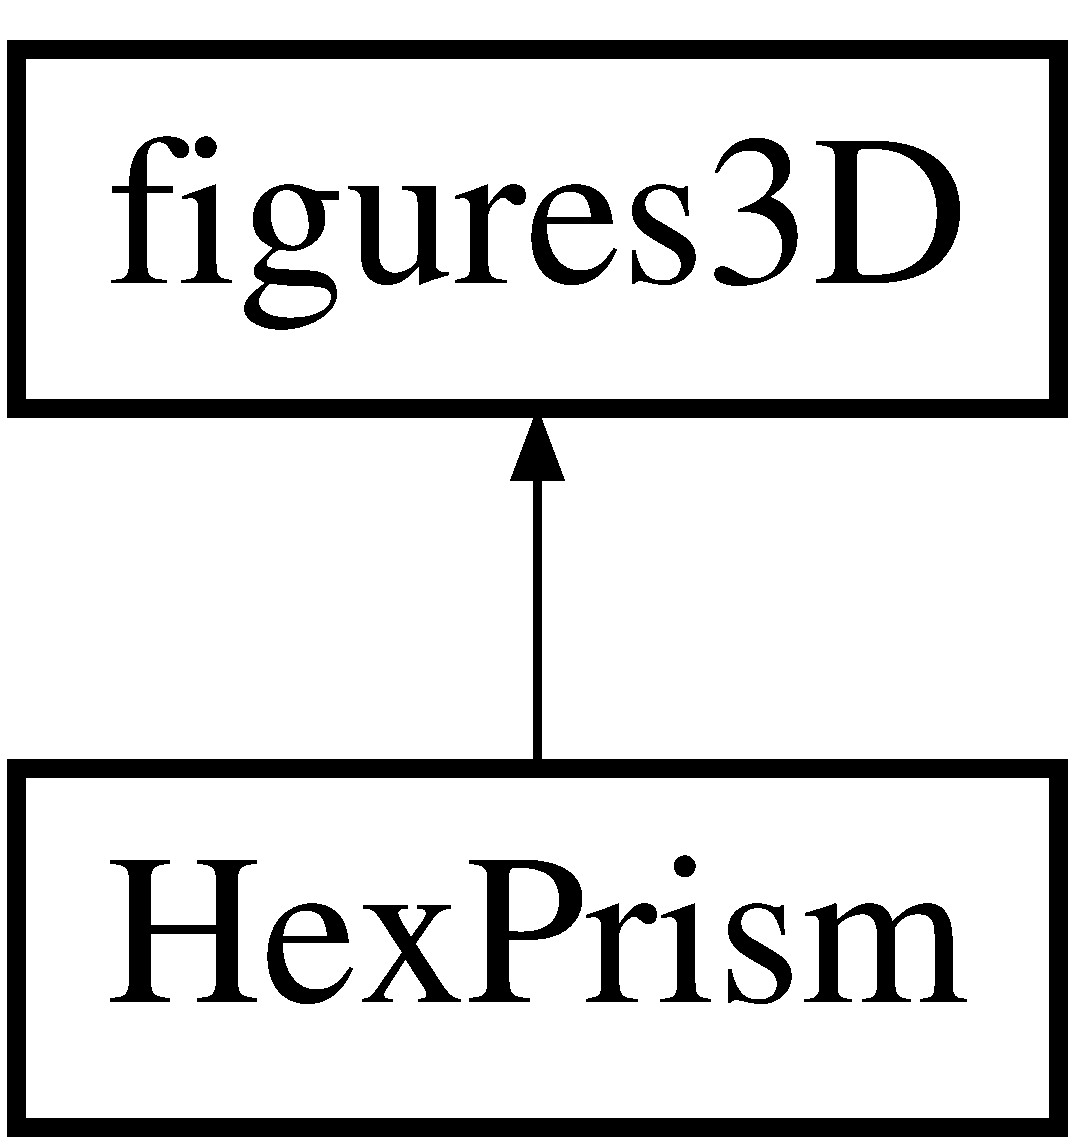
\includegraphics[height=2.000000cm]{class_hex_prism}
\end{center}
\end{figure}
\subsection*{Public Member Functions}
\begin{DoxyCompactItemize}
\item 
\hyperlink{class_hex_prism_a8360fd46ae716c1f5ba97f3213c3d223}{Hex\+Prism} (double x=0, double y=0, double z=0)
\begin{DoxyCompactList}\small\item\em Stworzenie nowego obiektu z mozliwoscia ustalenia jego polozenia na plaszczyznie xy. \end{DoxyCompactList}\item 
\hyperlink{vector3_d_8hh_a8790ef07836c1639da216f46501979c0}{Vector3D} \hyperlink{class_hex_prism_a9684bd167a9dcd710dbe227704bcb786}{Get\+Symetry\+Point} () const 
\begin{DoxyCompactList}\small\item\em Pobranie srodka symetrii graniastoslupa. \end{DoxyCompactList}\item 
void \hyperlink{class_hex_prism_a7d4bf4b9176fbb01146e74875d780626}{rotor} (bool side, \hyperlink{_hex_prism_8hh_ad57b3fa8e45359906ac229567c209a63}{Speed} speed)
\begin{DoxyCompactList}\small\item\em Rotowanie smigla podczas lotu. \end{DoxyCompactList}\end{DoxyCompactItemize}
\subsection*{Additional Inherited Members}


\subsection{Detailed Description}
Klasa wykorzystywana do sformulowania modelu smigla 

\subsection{Constructor \& Destructor Documentation}
\index{Hex\+Prism@{Hex\+Prism}!Hex\+Prism@{Hex\+Prism}}
\index{Hex\+Prism@{Hex\+Prism}!Hex\+Prism@{Hex\+Prism}}
\subsubsection[{\texorpdfstring{Hex\+Prism(double x=0, double y=0, double z=0)}{HexPrism(double x=0, double y=0, double z=0)}}]{\setlength{\rightskip}{0pt plus 5cm}Hex\+Prism\+::\+Hex\+Prism (
\begin{DoxyParamCaption}
\item[{double}]{x = {\ttfamily 0}, }
\item[{double}]{y = {\ttfamily 0}, }
\item[{double}]{z = {\ttfamily 0}}
\end{DoxyParamCaption}
)}\hypertarget{class_hex_prism_a8360fd46ae716c1f5ba97f3213c3d223}{}\label{class_hex_prism_a8360fd46ae716c1f5ba97f3213c3d223}

\begin{DoxyParams}{Parameters}
{\em x} & -\/ zmiana polozenia obiektu wedlug osi x \\
\hline
{\em y} & -\/ zmiana polozenia obiektu wedlug osi y \\
\hline
\end{DoxyParams}


\subsection{Member Function Documentation}
\index{Hex\+Prism@{Hex\+Prism}!Get\+Symetry\+Point@{Get\+Symetry\+Point}}
\index{Get\+Symetry\+Point@{Get\+Symetry\+Point}!Hex\+Prism@{Hex\+Prism}}
\subsubsection[{\texorpdfstring{Get\+Symetry\+Point() const }{GetSymetryPoint() const }}]{\setlength{\rightskip}{0pt plus 5cm}{\bf Vector3D} Hex\+Prism\+::\+Get\+Symetry\+Point (
\begin{DoxyParamCaption}
{}
\end{DoxyParamCaption}
) const}\hypertarget{class_hex_prism_a9684bd167a9dcd710dbe227704bcb786}{}\label{class_hex_prism_a9684bd167a9dcd710dbe227704bcb786}
Metoda przydatna przy przesuwaniu wspolrzednych do ukladu wspolrzednych danego graniastoslupa szesciokatnego

\begin{DoxyReturn}{Returns}
Vector3D -\/ srodek symetri graniastoslupa 
\end{DoxyReturn}
\index{Hex\+Prism@{Hex\+Prism}!rotor@{rotor}}
\index{rotor@{rotor}!Hex\+Prism@{Hex\+Prism}}
\subsubsection[{\texorpdfstring{rotor(bool side, Speed speed)}{rotor(bool side, Speed speed)}}]{\setlength{\rightskip}{0pt plus 5cm}void Hex\+Prism\+::rotor (
\begin{DoxyParamCaption}
\item[{bool}]{side, }
\item[{{\bf Speed}}]{speed}
\end{DoxyParamCaption}
)}\hypertarget{class_hex_prism_a7d4bf4b9176fbb01146e74875d780626}{}\label{class_hex_prism_a7d4bf4b9176fbb01146e74875d780626}
Rotujac smiglo najpierw przesuwamy uklad wspolrzednych do ukladu wspolrzednych graniastoskupa szeciokatnego dokonujemy rotacji, a nastepnie przywracamy bazowy uklad wspolrzednych


\begin{DoxyParams}{Parameters}
{\em side} & -\/ zmienna pomocna do ustalenia kierunku obrotu \mbox{[}lewo/prawo\mbox{]} \\
\hline
{\em speed} & -\/ szybkosc obrotu smigla \\
\hline
\end{DoxyParams}


The documentation for this class was generated from the following files\+:\begin{DoxyCompactItemize}
\item 
\hyperlink{_hex_prism_8hh}{Hex\+Prism.\+hh}\item 
\hyperlink{_hex_prism_8cpp}{Hex\+Prism.\+cpp}\end{DoxyCompactItemize}

\hypertarget{class_matrix}{}\section{Matrix$<$ Dimension $>$ Class Template Reference}
\label{class_matrix}\index{Matrix$<$ Dimension $>$@{Matrix$<$ Dimension $>$}}


Szablon modelujacy pojecie macierzy.  




{\ttfamily \#include $<$matrix.\+hh$>$}

\subsection*{Public Member Functions}
\begin{DoxyCompactItemize}
\item 
double \& \hyperlink{class_matrix_afff1ac83775f029d4bf9e472fff2b27e}{operator()} (int Index1, int Index2)
\begin{DoxyCompactList}\small\item\em Pobranie wartosci danego pola macierzy. \end{DoxyCompactList}\item 
double \hyperlink{class_matrix_a177a108c9b4631a0ef268c88b1aaf677}{operator()} (int Index1, int Index2) const 
\begin{DoxyCompactList}\small\item\em Pobranie wartosci danego pola macierzy bez mozliwosci modyfikacji tego pola. \end{DoxyCompactList}\item 
\hyperlink{class_matrix_ad3ddae5930748134cb331bf0bb508b86}{Matrix} ()
\begin{DoxyCompactList}\small\item\em Stworzenie nowego obiektu macierzy z przypisaniem zerowych wartosci. \end{DoxyCompactList}\item 
void \hyperlink{class_matrix_a25f743bb00f51eec66fc020f0600b2df}{Type\+\_\+\+In} (double alpha=1, char Choice\+Of\+Axix=\textquotesingle{}z\textquotesingle{})
\begin{DoxyCompactList}\small\item\em Wpsisanie odpowiednich wartosci do macierzy. \end{DoxyCompactList}\item 
\hyperlink{vector3_d_8hh_a8790ef07836c1639da216f46501979c0}{Vector3D} \hyperlink{class_matrix_a0db7f73a11fbe9a85d029d677c89582a}{operator$\ast$} (\hyperlink{vector3_d_8hh_a8790ef07836c1639da216f46501979c0}{Vector3D} \&vector) const 
\begin{DoxyCompactList}\small\item\em mnozenie wektora przez macierz \end{DoxyCompactList}\item 
\hyperlink{class_matrix}{Matrix}$<$ Dimension $>$ \hyperlink{class_matrix_a4a5436821ae1c3450d35803cb4d3c21d}{operator$\ast$} (\hyperlink{class_matrix}{Matrix}$<$ Dimension $>$ \&matrix2)
\begin{DoxyCompactList}\small\item\em Mnozenie dwoch macierzy. \end{DoxyCompactList}\end{DoxyCompactItemize}
\subsection*{Private Attributes}
\begin{DoxyCompactItemize}
\item 
double \hyperlink{class_matrix_a169e3264e9218b6881c8108db0cdf5c2}{a} \mbox{[}Dimension\mbox{]}\mbox{[}Dimension\mbox{]}
\begin{DoxyCompactList}\small\item\em Wspolrzedne macierzy przechowywane w dwuwymiarowej tablicy. \end{DoxyCompactList}\end{DoxyCompactItemize}


\subsection{Detailed Description}
\subsubsection*{template$<$int Dimension$>$\\*
class Matrix$<$ Dimension $>$}

Szablon modeluje pojecie macierzy,do ktorej mozemy wpisac odpowiednie wartosci Dzieki przeciazeniu operatorow () mozemy bezposrednio odwolac sie do pol macierzy reprezentowanych jako tablica 

\subsection{Constructor \& Destructor Documentation}
\index{Matrix@{Matrix}!Matrix@{Matrix}}
\index{Matrix@{Matrix}!Matrix@{Matrix}}
\subsubsection[{\texorpdfstring{Matrix()}{Matrix()}}]{\setlength{\rightskip}{0pt plus 5cm}template$<$int Dimension$>$ {\bf Matrix}$<$ Dimension $>$\+::{\bf Matrix} (
\begin{DoxyParamCaption}
{}
\end{DoxyParamCaption}
)\hspace{0.3cm}{\ttfamily [inline]}}\hypertarget{class_matrix_ad3ddae5930748134cb331bf0bb508b86}{}\label{class_matrix_ad3ddae5930748134cb331bf0bb508b86}


\subsection{Member Function Documentation}
\index{Matrix@{Matrix}!operator()@{operator()}}
\index{operator()@{operator()}!Matrix@{Matrix}}
\subsubsection[{\texorpdfstring{operator()(int Index1, int Index2)}{operator()(int Index1, int Index2)}}]{\setlength{\rightskip}{0pt plus 5cm}template$<$int Dimension$>$ double\& {\bf Matrix}$<$ Dimension $>$\+::operator() (
\begin{DoxyParamCaption}
\item[{int}]{Index1, }
\item[{int}]{Index2}
\end{DoxyParamCaption}
)\hspace{0.3cm}{\ttfamily [inline]}}\hypertarget{class_matrix_afff1ac83775f029d4bf9e472fff2b27e}{}\label{class_matrix_afff1ac83775f029d4bf9e472fff2b27e}

\begin{DoxyParams}{Parameters}
{\em Index1} & -\/ wiersz \\
\hline
{\em Index2} & -\/ kolumna \\
\hline
\end{DoxyParams}
\begin{DoxyReturn}{Returns}
double\& -\/ wartosc w danym polu, z mozliwoscia zmianny 
\end{DoxyReturn}
\index{Matrix@{Matrix}!operator()@{operator()}}
\index{operator()@{operator()}!Matrix@{Matrix}}
\subsubsection[{\texorpdfstring{operator()(int Index1, int Index2) const }{operator()(int Index1, int Index2) const }}]{\setlength{\rightskip}{0pt plus 5cm}template$<$int Dimension$>$ double {\bf Matrix}$<$ Dimension $>$\+::operator() (
\begin{DoxyParamCaption}
\item[{int}]{Index1, }
\item[{int}]{Index2}
\end{DoxyParamCaption}
) const\hspace{0.3cm}{\ttfamily [inline]}}\hypertarget{class_matrix_a177a108c9b4631a0ef268c88b1aaf677}{}\label{class_matrix_a177a108c9b4631a0ef268c88b1aaf677}

\begin{DoxyParams}{Parameters}
{\em Index1} & -\/ wiersz \\
\hline
{\em Index2} & -\/ kolumna \\
\hline
\end{DoxyParams}
\begin{DoxyReturn}{Returns}
double -\/ wartosc danego pola macierzy bez mozliwosci modyfikacji 
\end{DoxyReturn}
\index{Matrix@{Matrix}!operator$\ast$@{operator$\ast$}}
\index{operator$\ast$@{operator$\ast$}!Matrix@{Matrix}}
\subsubsection[{\texorpdfstring{operator$\ast$(\+Vector3\+D \&vector) const }{operator*(Vector3D &vector) const }}]{\setlength{\rightskip}{0pt plus 5cm}template$<$int Dimension$>$ {\bf Vector3D} {\bf Matrix}$<$ Dimension $>$\+::operator$\ast$ (
\begin{DoxyParamCaption}
\item[{{\bf Vector3D} \&}]{vector}
\end{DoxyParamCaption}
) const\hspace{0.3cm}{\ttfamily [inline]}}\hypertarget{class_matrix_a0db7f73a11fbe9a85d029d677c89582a}{}\label{class_matrix_a0db7f73a11fbe9a85d029d677c89582a}
mnozenie wektora przez macierz obrotu do ustalenia wspolrzednych po operacji rotacji


\begin{DoxyParams}{Parameters}
{\em vector} & -\/ mnozony wektor \\
\hline
\end{DoxyParams}
\begin{DoxyReturn}{Returns}
Vector3D -\/ przemnozony wektor 
\end{DoxyReturn}
\index{Matrix@{Matrix}!operator$\ast$@{operator$\ast$}}
\index{operator$\ast$@{operator$\ast$}!Matrix@{Matrix}}
\subsubsection[{\texorpdfstring{operator$\ast$(\+Matrix$<$ Dimension $>$ \&matrix2)}{operator*(Matrix< Dimension > &matrix2)}}]{\setlength{\rightskip}{0pt plus 5cm}template$<$int Dimension$>$ {\bf Matrix}$<$Dimension$>$ {\bf Matrix}$<$ Dimension $>$\+::operator$\ast$ (
\begin{DoxyParamCaption}
\item[{{\bf Matrix}$<$ Dimension $>$ \&}]{matrix2}
\end{DoxyParamCaption}
)\hspace{0.3cm}{\ttfamily [inline]}}\hypertarget{class_matrix_a4a5436821ae1c3450d35803cb4d3c21d}{}\label{class_matrix_a4a5436821ae1c3450d35803cb4d3c21d}

\begin{DoxyParams}{Parameters}
{\em matrix2} & -\/ drugi czynnik mnozenia, wymagane jest aby ten czynnik byl tych samych rozmiarow co pierwszy czynnik\\
\hline
\end{DoxyParams}
\begin{DoxyReturn}{Returns}
Matrix$<$\+Dimension$>$ -\/ przemnozona macierz 
\end{DoxyReturn}
\index{Matrix@{Matrix}!Type\+\_\+\+In@{Type\+\_\+\+In}}
\index{Type\+\_\+\+In@{Type\+\_\+\+In}!Matrix@{Matrix}}
\subsubsection[{\texorpdfstring{Type\+\_\+\+In(double alpha=1, char Choice\+Of\+Axix=\textquotesingle{}z\textquotesingle{})}{Type_In(double alpha=1, char ChoiceOfAxix='z')}}]{\setlength{\rightskip}{0pt plus 5cm}template$<$int Dimension$>$ void {\bf Matrix}$<$ Dimension $>$\+::Type\+\_\+\+In (
\begin{DoxyParamCaption}
\item[{double}]{alpha = {\ttfamily 1}, }
\item[{char}]{Choice\+Of\+Axix = {\ttfamily \textquotesingle{}z\textquotesingle{}}}
\end{DoxyParamCaption}
)\hspace{0.3cm}{\ttfamily [inline]}}\hypertarget{class_matrix_a25f743bb00f51eec66fc020f0600b2df}{}\label{class_matrix_a25f743bb00f51eec66fc020f0600b2df}
Funkcja na potrzeby macierzy 3 wymiarowej. Umozliwia wpisanie odpowiedniej macierzy obrotu(dla kazdej osi wartosci macierzy obrotu sa inne)


\begin{DoxyParams}{Parameters}
{\em alpha} & -\/ kat obrotu \\
\hline
{\em Choice\+Of\+Axix} & -\/ wybor osi obrotu \\
\hline
\end{DoxyParams}


\subsection{Member Data Documentation}
\index{Matrix@{Matrix}!a@{a}}
\index{a@{a}!Matrix@{Matrix}}
\subsubsection[{\texorpdfstring{a}{a}}]{\setlength{\rightskip}{0pt plus 5cm}template$<$int Dimension$>$ double {\bf Matrix}$<$ Dimension $>$\+::a\mbox{[}Dimension\mbox{]}\mbox{[}Dimension\mbox{]}\hspace{0.3cm}{\ttfamily [private]}}\hypertarget{class_matrix_a169e3264e9218b6881c8108db0cdf5c2}{}\label{class_matrix_a169e3264e9218b6881c8108db0cdf5c2}


The documentation for this class was generated from the following file\+:\begin{DoxyCompactItemize}
\item 
\hyperlink{matrix_8hh}{matrix.\+hh}\end{DoxyCompactItemize}

\hypertarget{class_object_of_scene}{}\section{Object\+Of\+Scene Class Reference}
\label{class_object_of_scene}\index{Object\+Of\+Scene@{Object\+Of\+Scene}}


Klasa bazowa dla drona i przeszkod.  




{\ttfamily \#include $<$Object\+Of\+Scene.\+hh$>$}

Inheritance diagram for Object\+Of\+Scene\+:\begin{figure}[H]
\begin{center}
\leavevmode
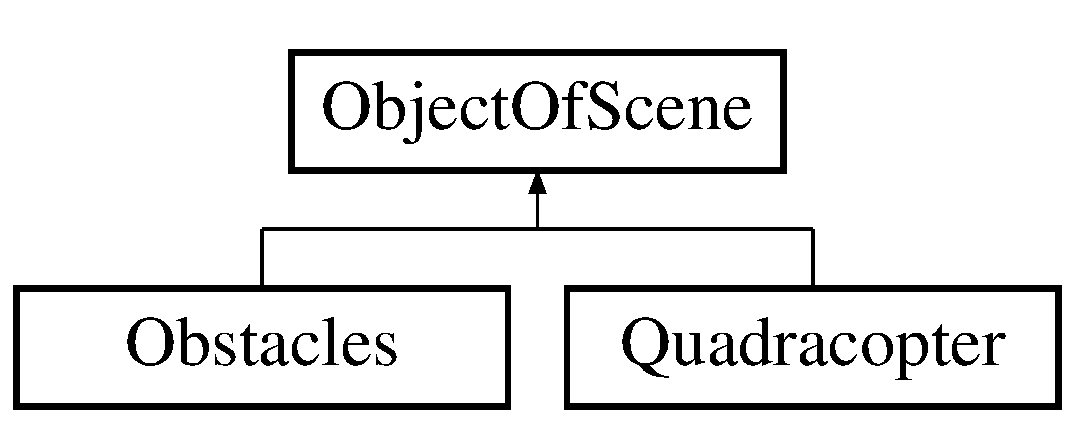
\includegraphics[height=2.000000cm]{class_object_of_scene}
\end{center}
\end{figure}
\subsection*{Public Member Functions}
\begin{DoxyCompactItemize}
\item 
\hyperlink{class_object_of_scene_a248118c01bc3c0b3df93bcc8ff4c169d}{Object\+Of\+Scene} ()
\begin{DoxyCompactList}\small\item\em Construct a new Object Of Scene object. \end{DoxyCompactList}\item 
virtual \hyperlink{class_object_of_scene_a1f973b6e583fe163630538a9da7caad8}{$\sim$\+Object\+Of\+Scene} ()
\begin{DoxyCompactList}\small\item\em Destroy the Object Of Scene object. \end{DoxyCompactList}\item 
\hyperlink{class_object_of_scene_a9dae6b015fdf9354b8f49235d10c439e}{Object\+Of\+Scene} (const \hyperlink{class_object_of_scene}{Object\+Of\+Scene} \&obj)
\begin{DoxyCompactList}\small\item\em Konstrktor kopiujacy. \end{DoxyCompactList}\item 
virtual bool \hyperlink{class_object_of_scene_ab58c09e26c9c6016fe86dcbd1b76df00}{If\+Collision} (\hyperlink{vector3_d_8hh_a8790ef07836c1639da216f46501979c0}{Vector3D} Physical\+Point, double radius) const 
\begin{DoxyCompactList}\small\item\em Sprawdzenie kolizji z obiektem. \end{DoxyCompactList}\item 
virtual bool \hyperlink{class_object_of_scene_a79bbabdf7e17459475bf30856cf176aa}{Write\+To\+File} (ofstream \&stream)
\begin{DoxyCompactList}\small\item\em Zapis do pliku obiektow sceny. \end{DoxyCompactList}\item 
\hyperlink{vector3_d_8hh_a8790ef07836c1639da216f46501979c0}{Vector3D} \& \hyperlink{class_object_of_scene_a1a2714bc1777bd167536f760fcd6c417}{Get\+Symetry} ()
\begin{DoxyCompactList}\small\item\em Pobranie punktu symetri. \end{DoxyCompactList}\end{DoxyCompactItemize}
\subsection*{Static Public Member Functions}
\begin{DoxyCompactItemize}
\item 
static void \hyperlink{class_object_of_scene_a94770327cfa3c391fbf6b8e4f9635248}{How\+Many\+Scene} ()
\begin{DoxyCompactList}\small\item\em Wypisanie ilosci obiektow sceny. \end{DoxyCompactList}\end{DoxyCompactItemize}
\subsection*{Static Public Attributes}
\begin{DoxyCompactItemize}
\item 
static int \hyperlink{class_object_of_scene_ae1b26e0c68453235a991601aa8f8c8e5}{counterS} =0
\begin{DoxyCompactList}\small\item\em Liczniki wystapien obiektow sceny. \end{DoxyCompactList}\item 
static int \hyperlink{class_object_of_scene_a4f29f829eca02965019b1d0bc28f3af1}{Add\+Counter} =0
\begin{DoxyCompactList}\small\item\em Calkowity licznik wystapien obiektow sceny. \end{DoxyCompactList}\end{DoxyCompactItemize}
\subsection*{Protected Attributes}
\begin{DoxyCompactItemize}
\item 
\hyperlink{vector3_d_8hh_a8790ef07836c1639da216f46501979c0}{Vector3D} \hyperlink{class_object_of_scene_a3940aba3014aefed326cdc4301333af1}{symetry}
\begin{DoxyCompactList}\small\item\em srodek symetri obiektu sceny \end{DoxyCompactList}\end{DoxyCompactItemize}


\subsection{Detailed Description}
Modeluje pojecie obiektu sceny, przypisuje mu srodek symetri 

\subsection{Constructor \& Destructor Documentation}
\index{Object\+Of\+Scene@{Object\+Of\+Scene}!Object\+Of\+Scene@{Object\+Of\+Scene}}
\index{Object\+Of\+Scene@{Object\+Of\+Scene}!Object\+Of\+Scene@{Object\+Of\+Scene}}
\subsubsection[{\texorpdfstring{Object\+Of\+Scene()}{ObjectOfScene()}}]{\setlength{\rightskip}{0pt plus 5cm}Object\+Of\+Scene\+::\+Object\+Of\+Scene (
\begin{DoxyParamCaption}
{}
\end{DoxyParamCaption}
)\hspace{0.3cm}{\ttfamily [inline]}}\hypertarget{class_object_of_scene_a248118c01bc3c0b3df93bcc8ff4c169d}{}\label{class_object_of_scene_a248118c01bc3c0b3df93bcc8ff4c169d}
\index{Object\+Of\+Scene@{Object\+Of\+Scene}!````~Object\+Of\+Scene@{$\sim$\+Object\+Of\+Scene}}
\index{````~Object\+Of\+Scene@{$\sim$\+Object\+Of\+Scene}!Object\+Of\+Scene@{Object\+Of\+Scene}}
\subsubsection[{\texorpdfstring{$\sim$\+Object\+Of\+Scene()}{~ObjectOfScene()}}]{\setlength{\rightskip}{0pt plus 5cm}virtual Object\+Of\+Scene\+::$\sim$\+Object\+Of\+Scene (
\begin{DoxyParamCaption}
{}
\end{DoxyParamCaption}
)\hspace{0.3cm}{\ttfamily [inline]}, {\ttfamily [virtual]}}\hypertarget{class_object_of_scene_a1f973b6e583fe163630538a9da7caad8}{}\label{class_object_of_scene_a1f973b6e583fe163630538a9da7caad8}
\index{Object\+Of\+Scene@{Object\+Of\+Scene}!Object\+Of\+Scene@{Object\+Of\+Scene}}
\index{Object\+Of\+Scene@{Object\+Of\+Scene}!Object\+Of\+Scene@{Object\+Of\+Scene}}
\subsubsection[{\texorpdfstring{Object\+Of\+Scene(const Object\+Of\+Scene \&obj)}{ObjectOfScene(const ObjectOfScene &obj)}}]{\setlength{\rightskip}{0pt plus 5cm}Object\+Of\+Scene\+::\+Object\+Of\+Scene (
\begin{DoxyParamCaption}
\item[{const {\bf Object\+Of\+Scene} \&}]{obj}
\end{DoxyParamCaption}
)\hspace{0.3cm}{\ttfamily [inline]}}\hypertarget{class_object_of_scene_a9dae6b015fdf9354b8f49235d10c439e}{}\label{class_object_of_scene_a9dae6b015fdf9354b8f49235d10c439e}

\begin{DoxyParams}{Parameters}
{\em obj} & -\/ obiekt sceny \\
\hline
\end{DoxyParams}


\subsection{Member Function Documentation}
\index{Object\+Of\+Scene@{Object\+Of\+Scene}!Get\+Symetry@{Get\+Symetry}}
\index{Get\+Symetry@{Get\+Symetry}!Object\+Of\+Scene@{Object\+Of\+Scene}}
\subsubsection[{\texorpdfstring{Get\+Symetry()}{GetSymetry()}}]{\setlength{\rightskip}{0pt plus 5cm}{\bf Vector3D}\& Object\+Of\+Scene\+::\+Get\+Symetry (
\begin{DoxyParamCaption}
{}
\end{DoxyParamCaption}
)\hspace{0.3cm}{\ttfamily [inline]}}\hypertarget{class_object_of_scene_a1a2714bc1777bd167536f760fcd6c417}{}\label{class_object_of_scene_a1a2714bc1777bd167536f760fcd6c417}
\begin{DoxyReturn}{Returns}
Vector3D\& -\/ punkt symetri 
\end{DoxyReturn}
\index{Object\+Of\+Scene@{Object\+Of\+Scene}!How\+Many\+Scene@{How\+Many\+Scene}}
\index{How\+Many\+Scene@{How\+Many\+Scene}!Object\+Of\+Scene@{Object\+Of\+Scene}}
\subsubsection[{\texorpdfstring{How\+Many\+Scene()}{HowManyScene()}}]{\setlength{\rightskip}{0pt plus 5cm}static void Object\+Of\+Scene\+::\+How\+Many\+Scene (
\begin{DoxyParamCaption}
{}
\end{DoxyParamCaption}
)\hspace{0.3cm}{\ttfamily [inline]}, {\ttfamily [static]}}\hypertarget{class_object_of_scene_a94770327cfa3c391fbf6b8e4f9635248}{}\label{class_object_of_scene_a94770327cfa3c391fbf6b8e4f9635248}
\index{Object\+Of\+Scene@{Object\+Of\+Scene}!If\+Collision@{If\+Collision}}
\index{If\+Collision@{If\+Collision}!Object\+Of\+Scene@{Object\+Of\+Scene}}
\subsubsection[{\texorpdfstring{If\+Collision(\+Vector3\+D Physical\+Point, double radius) const }{IfCollision(Vector3D PhysicalPoint, double radius) const }}]{\setlength{\rightskip}{0pt plus 5cm}virtual bool Object\+Of\+Scene\+::\+If\+Collision (
\begin{DoxyParamCaption}
\item[{{\bf Vector3D}}]{Physical\+Point, }
\item[{double}]{radius}
\end{DoxyParamCaption}
) const\hspace{0.3cm}{\ttfamily [inline]}, {\ttfamily [virtual]}}\hypertarget{class_object_of_scene_ab58c09e26c9c6016fe86dcbd1b76df00}{}\label{class_object_of_scene_ab58c09e26c9c6016fe86dcbd1b76df00}

\begin{DoxyParams}{Parameters}
{\em Physical\+Point} & -\/ srodek symetri wybranego drona \\
\hline
{\em radius} & -\/ promien \\
\hline
\end{DoxyParams}
\begin{DoxyReturn}{Returns}
true -\/ jest kolizja 

false -\/ nie ma kolizji 
\end{DoxyReturn}


Reimplemented in \hyperlink{class_quadracopter_a27a2a987ddd033cdc774dbdd1a28d153}{Quadracopter}, and \hyperlink{class_obstacles_a873ae714db7bf22195867aed06e72227}{Obstacles}.

\index{Object\+Of\+Scene@{Object\+Of\+Scene}!Write\+To\+File@{Write\+To\+File}}
\index{Write\+To\+File@{Write\+To\+File}!Object\+Of\+Scene@{Object\+Of\+Scene}}
\subsubsection[{\texorpdfstring{Write\+To\+File(ofstream \&stream)}{WriteToFile(ofstream &stream)}}]{\setlength{\rightskip}{0pt plus 5cm}virtual bool Object\+Of\+Scene\+::\+Write\+To\+File (
\begin{DoxyParamCaption}
\item[{ofstream \&}]{stream}
\end{DoxyParamCaption}
)\hspace{0.3cm}{\ttfamily [inline]}, {\ttfamily [virtual]}}\hypertarget{class_object_of_scene_a79bbabdf7e17459475bf30856cf176aa}{}\label{class_object_of_scene_a79bbabdf7e17459475bf30856cf176aa}
Dla kazdego obiektu zapis uzywa innego przeciazenia dlatego ta metoda jest wirtualna


\begin{DoxyParams}{Parameters}
{\em stream} & -\/ strumien do zapisu \\
\hline
\end{DoxyParams}
\begin{DoxyReturn}{Returns}
true -\/ udany zapis 

false -\/ nieudany zapis 
\end{DoxyReturn}


Reimplemented in \hyperlink{class_quadracopter_a0653c1a4019907005c4d758168ad2ec1}{Quadracopter}, and \hyperlink{class_obstacles_a41b1c2255c6230514fb6a91afb5f8f7b}{Obstacles}.



\subsection{Member Data Documentation}
\index{Object\+Of\+Scene@{Object\+Of\+Scene}!Add\+Counter@{Add\+Counter}}
\index{Add\+Counter@{Add\+Counter}!Object\+Of\+Scene@{Object\+Of\+Scene}}
\subsubsection[{\texorpdfstring{Add\+Counter}{AddCounter}}]{\setlength{\rightskip}{0pt plus 5cm}int Object\+Of\+Scene\+::\+Add\+Counter =0\hspace{0.3cm}{\ttfamily [static]}}\hypertarget{class_object_of_scene_a4f29f829eca02965019b1d0bc28f3af1}{}\label{class_object_of_scene_a4f29f829eca02965019b1d0bc28f3af1}
Inicjalizacja licznika wszystkich wystapien obiektow. \index{Object\+Of\+Scene@{Object\+Of\+Scene}!counterS@{counterS}}
\index{counterS@{counterS}!Object\+Of\+Scene@{Object\+Of\+Scene}}
\subsubsection[{\texorpdfstring{counterS}{counterS}}]{\setlength{\rightskip}{0pt plus 5cm}int Object\+Of\+Scene\+::counterS =0\hspace{0.3cm}{\ttfamily [static]}}\hypertarget{class_object_of_scene_ae1b26e0c68453235a991601aa8f8c8e5}{}\label{class_object_of_scene_ae1b26e0c68453235a991601aa8f8c8e5}
Inicjalizacja licznika. \index{Object\+Of\+Scene@{Object\+Of\+Scene}!symetry@{symetry}}
\index{symetry@{symetry}!Object\+Of\+Scene@{Object\+Of\+Scene}}
\subsubsection[{\texorpdfstring{symetry}{symetry}}]{\setlength{\rightskip}{0pt plus 5cm}{\bf Vector3D} Object\+Of\+Scene\+::symetry\hspace{0.3cm}{\ttfamily [protected]}}\hypertarget{class_object_of_scene_a3940aba3014aefed326cdc4301333af1}{}\label{class_object_of_scene_a3940aba3014aefed326cdc4301333af1}


The documentation for this class was generated from the following files\+:\begin{DoxyCompactItemize}
\item 
\hyperlink{_object_of_scene_8hh}{Object\+Of\+Scene.\+hh}\item 
\hyperlink{_object_of_scene_8cpp}{Object\+Of\+Scene.\+cpp}\end{DoxyCompactItemize}

\hypertarget{class_obstacles}{}\section{Obstacles Class Reference}
\label{class_obstacles}\index{Obstacles@{Obstacles}}


Klasa modeluje pojecie przeszkody na scenie.  




{\ttfamily \#include $<$Obstacles.\+hh$>$}

Inheritance diagram for Obstacles\+:\begin{figure}[H]
\begin{center}
\leavevmode
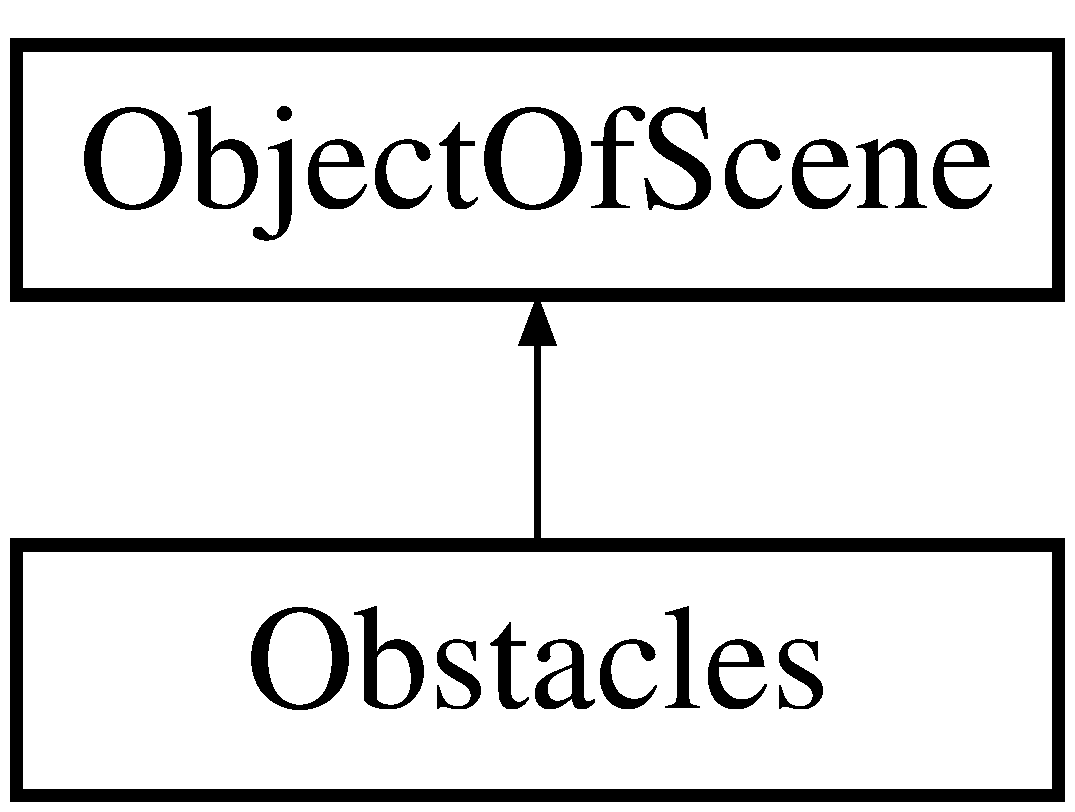
\includegraphics[height=2.000000cm]{class_obstacles}
\end{center}
\end{figure}
\subsection*{Public Member Functions}
\begin{DoxyCompactItemize}
\item 
\hyperlink{class_obstacles_a51c7f97c28a251ab75d711b23d9fe8e1}{Obstacles} ()
\begin{DoxyCompactList}\small\item\em Construct a new \hyperlink{class_obstacles}{Obstacles} object. \end{DoxyCompactList}\item 
\hyperlink{class_obstacles_a28b7f32500e1e58465ef5dc9e2d63ec1}{Obstacles} (\hyperlink{vector3_d_8hh_a8790ef07836c1639da216f46501979c0}{Vector3D} centre, \hyperlink{vector3_d_8hh_a8790ef07836c1639da216f46501979c0}{Vector3D} size)
\begin{DoxyCompactList}\small\item\em Construct a new \hyperlink{class_obstacles}{Obstacles} object. \end{DoxyCompactList}\item 
\hyperlink{class_cuboid}{Cuboid} \hyperlink{class_obstacles_aacee9a8a19128a528e2b236485030128}{Get\+Obstacle} ()
\begin{DoxyCompactList}\small\item\em Dobranie sie do przeszkody. \end{DoxyCompactList}\item 
bool \hyperlink{class_obstacles_a873ae714db7bf22195867aed06e72227}{If\+Collision} (\hyperlink{vector3_d_8hh_a8790ef07836c1639da216f46501979c0}{Vector3D} Physical\+Point, double radius) const 
\begin{DoxyCompactList}\small\item\em Sprawdzanie kolizji z obiektami. \end{DoxyCompactList}\item 
bool \hyperlink{class_obstacles_a41b1c2255c6230514fb6a91afb5f8f7b}{Write\+To\+File} (ofstream \&stream)
\begin{DoxyCompactList}\small\item\em Zapis przeszkody do pliku. \end{DoxyCompactList}\end{DoxyCompactItemize}
\subsection*{Private Attributes}
\begin{DoxyCompactItemize}
\item 
\hyperlink{class_cuboid}{Cuboid} \hyperlink{class_obstacles_a524ef2c37e9160887bd20780d68cff76}{cub}
\begin{DoxyCompactList}\small\item\em Przeszkody sa wizualizowane za pomoca prostopadloscianow. \end{DoxyCompactList}\end{DoxyCompactItemize}
\subsection*{Additional Inherited Members}


\subsection{Constructor \& Destructor Documentation}
\index{Obstacles@{Obstacles}!Obstacles@{Obstacles}}
\index{Obstacles@{Obstacles}!Obstacles@{Obstacles}}
\subsubsection[{\texorpdfstring{Obstacles()}{Obstacles()}}]{\setlength{\rightskip}{0pt plus 5cm}Obstacles\+::\+Obstacles (
\begin{DoxyParamCaption}
{}
\end{DoxyParamCaption}
)\hspace{0.3cm}{\ttfamily [inline]}}\hypertarget{class_obstacles_a51c7f97c28a251ab75d711b23d9fe8e1}{}\label{class_obstacles_a51c7f97c28a251ab75d711b23d9fe8e1}
\index{Obstacles@{Obstacles}!Obstacles@{Obstacles}}
\index{Obstacles@{Obstacles}!Obstacles@{Obstacles}}
\subsubsection[{\texorpdfstring{Obstacles(\+Vector3\+D centre, Vector3\+D size)}{Obstacles(Vector3D centre, Vector3D size)}}]{\setlength{\rightskip}{0pt plus 5cm}Obstacles\+::\+Obstacles (
\begin{DoxyParamCaption}
\item[{{\bf Vector3D}}]{centre, }
\item[{{\bf Vector3D}}]{size}
\end{DoxyParamCaption}
)}\hypertarget{class_obstacles_a28b7f32500e1e58465ef5dc9e2d63ec1}{}\label{class_obstacles_a28b7f32500e1e58465ef5dc9e2d63ec1}

\begin{DoxyParams}{Parameters}
{\em centre} & -\/ srodek symetrii przeszkody \\
\hline
{\em size} & -\/ rozmiary przeszkody \\
\hline
\end{DoxyParams}


\subsection{Member Function Documentation}
\index{Obstacles@{Obstacles}!Get\+Obstacle@{Get\+Obstacle}}
\index{Get\+Obstacle@{Get\+Obstacle}!Obstacles@{Obstacles}}
\subsubsection[{\texorpdfstring{Get\+Obstacle()}{GetObstacle()}}]{\setlength{\rightskip}{0pt plus 5cm}{\bf Cuboid} Obstacles\+::\+Get\+Obstacle (
\begin{DoxyParamCaption}
{}
\end{DoxyParamCaption}
)\hspace{0.3cm}{\ttfamily [inline]}}\hypertarget{class_obstacles_aacee9a8a19128a528e2b236485030128}{}\label{class_obstacles_aacee9a8a19128a528e2b236485030128}

\begin{DoxyParams}{Parameters}
{\em Index} & -\/ numer przeszkody \\
\hline
\end{DoxyParams}
\begin{DoxyReturn}{Returns}
\hyperlink{class_cuboid}{Cuboid} -\/ przeszkoda 
\end{DoxyReturn}
\index{Obstacles@{Obstacles}!If\+Collision@{If\+Collision}}
\index{If\+Collision@{If\+Collision}!Obstacles@{Obstacles}}
\subsubsection[{\texorpdfstring{If\+Collision(\+Vector3\+D Physical\+Point, double radius) const }{IfCollision(Vector3D PhysicalPoint, double radius) const }}]{\setlength{\rightskip}{0pt plus 5cm}bool Obstacles\+::\+If\+Collision (
\begin{DoxyParamCaption}
\item[{{\bf Vector3D}}]{Physical\+Point, }
\item[{double}]{radius}
\end{DoxyParamCaption}
) const\hspace{0.3cm}{\ttfamily [virtual]}}\hypertarget{class_obstacles_a873ae714db7bf22195867aed06e72227}{}\label{class_obstacles_a873ae714db7bf22195867aed06e72227}

\begin{DoxyParams}{Parameters}
{\em Physical\+Point} & -\/ srodek symetri wybranego drona \\
\hline
{\em radius} & -\/ promien walca przyblizajacego \\
\hline
\end{DoxyParams}
\begin{DoxyReturn}{Returns}
true -\/ detekcja kolizji 

false -\/ nie ma kolizji 
\end{DoxyReturn}


Reimplemented from \hyperlink{class_object_of_scene_ab58c09e26c9c6016fe86dcbd1b76df00}{Object\+Of\+Scene}.

\index{Obstacles@{Obstacles}!Write\+To\+File@{Write\+To\+File}}
\index{Write\+To\+File@{Write\+To\+File}!Obstacles@{Obstacles}}
\subsubsection[{\texorpdfstring{Write\+To\+File(ofstream \&stream)}{WriteToFile(ofstream &stream)}}]{\setlength{\rightskip}{0pt plus 5cm}bool Obstacles\+::\+Write\+To\+File (
\begin{DoxyParamCaption}
\item[{ofstream \&}]{stream}
\end{DoxyParamCaption}
)\hspace{0.3cm}{\ttfamily [virtual]}}\hypertarget{class_obstacles_a41b1c2255c6230514fb6a91afb5f8f7b}{}\label{class_obstacles_a41b1c2255c6230514fb6a91afb5f8f7b}

\begin{DoxyParams}{Parameters}
{\em stream} & -\/ strumien do zapisu \\
\hline
\end{DoxyParams}
\begin{DoxyReturn}{Returns}
true -\/ udany zapis 

false -\/ nieudany zapis 
\end{DoxyReturn}


Reimplemented from \hyperlink{class_object_of_scene_a79bbabdf7e17459475bf30856cf176aa}{Object\+Of\+Scene}.



\subsection{Member Data Documentation}
\index{Obstacles@{Obstacles}!cub@{cub}}
\index{cub@{cub}!Obstacles@{Obstacles}}
\subsubsection[{\texorpdfstring{cub}{cub}}]{\setlength{\rightskip}{0pt plus 5cm}{\bf Cuboid} Obstacles\+::cub\hspace{0.3cm}{\ttfamily [private]}}\hypertarget{class_obstacles_a524ef2c37e9160887bd20780d68cff76}{}\label{class_obstacles_a524ef2c37e9160887bd20780d68cff76}


The documentation for this class was generated from the following files\+:\begin{DoxyCompactItemize}
\item 
\hyperlink{_obstacles_8hh}{Obstacles.\+hh}\item 
\hyperlink{_obstacles_8cpp}{Obstacles.\+cpp}\end{DoxyCompactItemize}

\hypertarget{class_plant_of_obstacles}{}\section{Plant\+Of\+Obstacles Class Reference}
\label{class_plant_of_obstacles}\index{Plant\+Of\+Obstacles@{Plant\+Of\+Obstacles}}


Klasa modeluje pojecie fabryki obiektow.  




{\ttfamily \#include $<$Plant\+Of\+Obstacles.\+hh$>$}

\subsection*{Public Member Functions}
\begin{DoxyCompactItemize}
\item 
shared\+\_\+ptr$<$ \hyperlink{class_object_of_scene}{Object\+Of\+Scene} $>$ \hyperlink{class_plant_of_obstacles_aed9fac6bbe259c61e016d1d8ad812b87}{Add\+Object} (\hyperlink{_plant_of_obstacles_8hh_a094c367727273b4da2b960ca3b3edc06}{ID} id, \hyperlink{_plant_of_obstacles_8hh_a4c502dc6ce14797e2bb86775ccf09cbf}{Users} users) const 
\begin{DoxyCompactList}\small\item\em Metoda tworzaca nowy obiekt. \end{DoxyCompactList}\end{DoxyCompactItemize}


\subsection{Detailed Description}
Tyllko tutaj mozliwe jest tworzenie obiektow klasy przeszkoda oraz dron 

\subsection{Member Function Documentation}
\index{Plant\+Of\+Obstacles@{Plant\+Of\+Obstacles}!Add\+Object@{Add\+Object}}
\index{Add\+Object@{Add\+Object}!Plant\+Of\+Obstacles@{Plant\+Of\+Obstacles}}
\subsubsection[{\texorpdfstring{Add\+Object(\+I\+D id, Users users) const }{AddObject(ID id, Users users) const }}]{\setlength{\rightskip}{0pt plus 5cm}shared\+\_\+ptr$<$ {\bf Object\+Of\+Scene} $>$ Plant\+Of\+Obstacles\+::\+Add\+Object (
\begin{DoxyParamCaption}
\item[{{\bf ID}}]{id, }
\item[{{\bf Users}}]{users}
\end{DoxyParamCaption}
) const}\hypertarget{class_plant_of_obstacles_aed9fac6bbe259c61e016d1d8ad812b87}{}\label{class_plant_of_obstacles_aed9fac6bbe259c61e016d1d8ad812b87}

\begin{DoxyParams}{Parameters}
{\em id} & -\/ identyfikator obiektu (Dron lub przeszkoda) \\
\hline
{\em users} & -\/ uzytkownik ktory tworzy obiekt \\
\hline
\end{DoxyParams}
\begin{DoxyReturn}{Returns}
shared\+\_\+ptr$<$\+Object\+Of\+Scene$>$ -\/ nowy stworzony obiekt zrzutowany na obiekt sceny 
\end{DoxyReturn}


The documentation for this class was generated from the following files\+:\begin{DoxyCompactItemize}
\item 
\hyperlink{_plant_of_obstacles_8hh}{Plant\+Of\+Obstacles.\+hh}\item 
\hyperlink{_plant_of_obstacles_8cpp}{Plant\+Of\+Obstacles.\+cpp}\end{DoxyCompactItemize}

\hypertarget{class_quadracopter}{}\section{Quadracopter Class Reference}
\label{class_quadracopter}\index{Quadracopter@{Quadracopter}}


Model pojecia dron.  




{\ttfamily \#include $<$Quadracopter.\+hh$>$}

Inheritance diagram for Quadracopter\+:\begin{figure}[H]
\begin{center}
\leavevmode
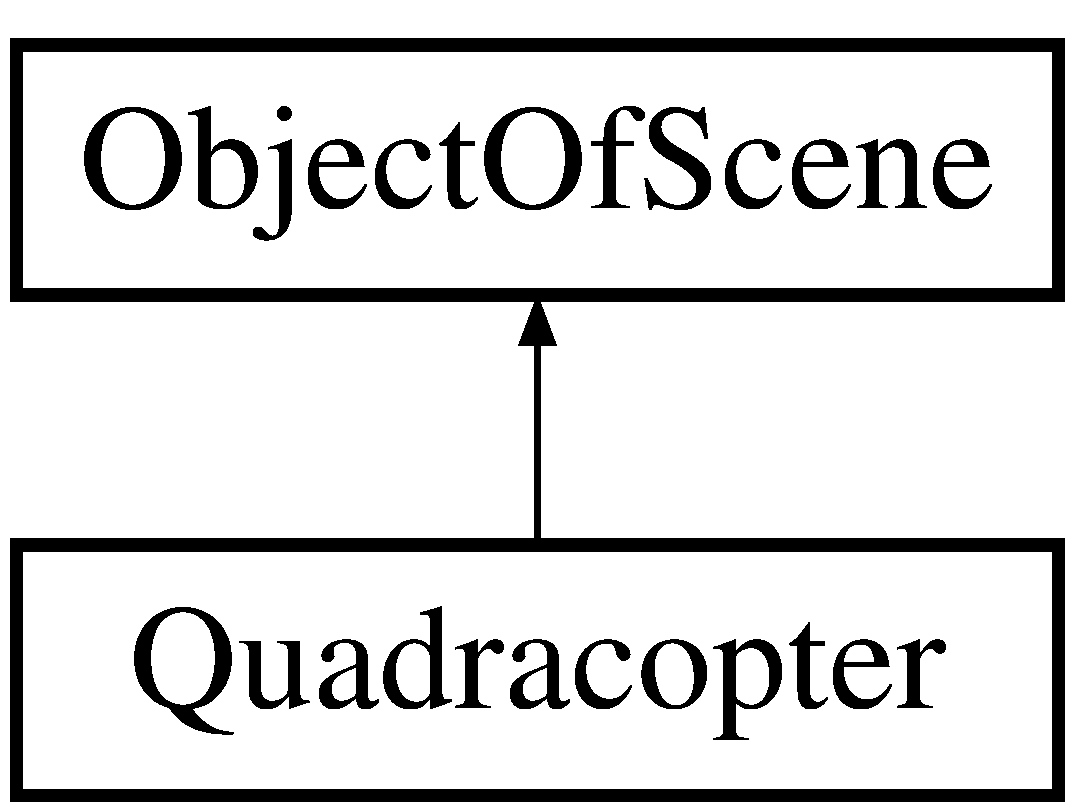
\includegraphics[height=2.000000cm]{class_quadracopter}
\end{center}
\end{figure}
\subsection*{Public Member Functions}
\begin{DoxyCompactItemize}
\item 
void \hyperlink{class_quadracopter_ac9bed2c9c204a7f260fec4f1f71e3402}{Change\+Orientation} (\hyperlink{matrix3x3_8hh_ae0d6db325717593a1d1157ecfa156f13}{Matrix3x3} matrix, \hyperlink{vector3_d_8hh_a8790ef07836c1639da216f46501979c0}{Vector3D} \hyperlink{class_object_of_scene_a3940aba3014aefed326cdc4301333af1}{symetry})
\begin{DoxyCompactList}\small\item\em Zmiana kazdego wierzcholka o zadany kat obrotu. \end{DoxyCompactList}\item 
\hyperlink{class_quadracopter_a9acb965be075b277df0901e99cccfacf}{Quadracopter} ()
\begin{DoxyCompactList}\small\item\em Stworzenie drona z automatycznym przypisaniem wierzcholkow. \end{DoxyCompactList}\item 
\hyperlink{class_quadracopter_a53ea4afb198dee646fa391296b00da48}{Quadracopter} (double x, double y, double z)
\begin{DoxyCompactList}\small\item\em Konstruktor parametryczny z zadanym wektorem przesuniecia. \end{DoxyCompactList}\item 
\hyperlink{class_cuboid}{Cuboid} \& \hyperlink{class_quadracopter_a1e565e85a55c6c2c1ea7db8869dd6dcc}{Get\+Hull} ()
\begin{DoxyCompactList}\small\item\em Pobranie kadluba z mozliwoscia zmiany. \end{DoxyCompactList}\item 
\hyperlink{class_cuboid}{Cuboid} \hyperlink{class_quadracopter_a331af4fd71ff51021a1787d8a4bef657}{Get\+Hull} () const 
\begin{DoxyCompactList}\small\item\em Pobranie kadluba bez mozliwosci dokonywania zmian. \end{DoxyCompactList}\item 
\hyperlink{class_hex_prism}{Hex\+Prism} \& \hyperlink{class_quadracopter_a48018a30c1ea5706c41dffee4214cd2a}{operator\mbox{[}$\,$\mbox{]}} (int Index)
\begin{DoxyCompactList}\small\item\em 
\begin{DoxyItemize}
\item Pobranie smigiel z mozliowscia modyfikacji 
\end{DoxyItemize}\end{DoxyCompactList}\item 
\hyperlink{class_hex_prism}{Hex\+Prism} \hyperlink{class_quadracopter_a35db9425da009e00a6fc4b0393b0d3fb}{operator\mbox{[}$\,$\mbox{]}} (int Index) const 
\begin{DoxyCompactList}\small\item\em Pobranie smigla bez mozliwosci modyfikacji. \end{DoxyCompactList}\item 
void \hyperlink{class_quadracopter_ac4aedc67a3d57345721978acdec6ee18}{Add\+Angle} (int value)
\begin{DoxyCompactList}\small\item\em zapamietanie katu obrotu \end{DoxyCompactList}\item 
double \hyperlink{class_quadracopter_a1e43b7fba5785f94e451f1510c7be5e1}{Get\+Angle} () const 
\begin{DoxyCompactList}\small\item\em pobranie sumarycznego kata obrout \end{DoxyCompactList}\item 
\hyperlink{vector3_d_8hh_a8790ef07836c1639da216f46501979c0}{Vector3D} \hyperlink{class_quadracopter_a88854bf826c6ee95de12947ae45112cb}{Move\+Up\+Down} (double angle) const 
\begin{DoxyCompactList}\small\item\em Wyliczenie wektora translacji. \end{DoxyCompactList}\item 
bool \hyperlink{class_quadracopter_a27a2a987ddd033cdc774dbdd1a28d153}{If\+Collision} (\hyperlink{vector3_d_8hh_a8790ef07836c1639da216f46501979c0}{Vector3D} Physical\+Point, double \hyperlink{class_quadracopter_a34736716e6c9c1ef8a73dec7e4dc2485}{radius}) const 
\begin{DoxyCompactList}\small\item\em Sprawdzanie kolizji z dronem. \end{DoxyCompactList}\item 
double \& \hyperlink{class_quadracopter_ac511e0187c27f49c0e43bcb1512f0941}{Get\+Radius} ()
\begin{DoxyCompactList}\small\item\em Pobierz promien walca. \end{DoxyCompactList}\item 
double \& \hyperlink{class_quadracopter_aa8bc9fd45eb2b63505ae29673a9e157d}{Get\+Height} ()
\begin{DoxyCompactList}\small\item\em Pobierz pol wysokosci walca. \end{DoxyCompactList}\item 
\hyperlink{vector3_d_8hh_a8790ef07836c1639da216f46501979c0}{Vector3D} \hyperlink{class_quadracopter_aa1c2a6f507a5bcd7bc37fa5d44a930e5}{Move\+Symetry} ()
\begin{DoxyCompactList}\small\item\em Zmiana wspolrzednych srodka symetri ( punktu materialnego) podczas przemieszczania/rotacji. \end{DoxyCompactList}\item 
list$<$ \hyperlink{vector3_d_8hh_a8790ef07836c1639da216f46501979c0}{Vector3D} $>$ \& \hyperlink{class_quadracopter_a8b7c6b9d441156f3991b11b73543adc3}{Get\+Track} ()
\begin{DoxyCompactList}\small\item\em Pobranie trasy. \end{DoxyCompactList}\item 
bool \hyperlink{class_quadracopter_a0653c1a4019907005c4d758168ad2ec1}{Write\+To\+File} (ofstream \&stream)
\begin{DoxyCompactList}\small\item\em Zapis drona do pliku. \end{DoxyCompactList}\end{DoxyCompactItemize}
\subsection*{Private Attributes}
\begin{DoxyCompactItemize}
\item 
\hyperlink{class_cuboid}{Cuboid} \hyperlink{class_quadracopter_a1bc37defc8b79a02c1abba10e69742a7}{hull}
\begin{DoxyCompactList}\small\item\em kadlub drona reprezentowany jako prostopadloscian+ \end{DoxyCompactList}\item 
\hyperlink{class_hex_prism}{Hex\+Prism} \hyperlink{class_quadracopter_a51b2350b8ec3efc0906228595ffcecd1}{disc} \mbox{[}\hyperlink{_quadracopter_8hh_ae118ca9ee93d6a5f2588b28d39dee76b}{k\+Number\+Of\+Disc}\mbox{]}
\begin{DoxyCompactList}\small\item\em smigla drona reprezentowane przez graniastoslup szeciokatny \end{DoxyCompactList}\item 
double \hyperlink{class_quadracopter_a2d2329d63abb5ff624dc1d95660a08b4}{Rotation\+Angle}
\begin{DoxyCompactList}\small\item\em sumaryczny kat obrotu \end{DoxyCompactList}\item 
double \hyperlink{class_quadracopter_a34736716e6c9c1ef8a73dec7e4dc2485}{radius}
\begin{DoxyCompactList}\small\item\em Promien walca przyblizajacego dron. \end{DoxyCompactList}\item 
double \hyperlink{class_quadracopter_aebaeeec3692eeff5e6d51549e9eb0619}{height}
\begin{DoxyCompactList}\small\item\em polowa dlugosci walca przyblizajacego dron \end{DoxyCompactList}\item 
list$<$ \hyperlink{vector3_d_8hh_a8790ef07836c1639da216f46501979c0}{Vector3D} $>$ \hyperlink{class_quadracopter_a04bd01dc2756f344af906ffb4f8b6655}{track}
\begin{DoxyCompactList}\small\item\em Sciezka/\+Trasa jako lista punktow. \end{DoxyCompactList}\end{DoxyCompactItemize}
\subsection*{Friends}
\begin{DoxyCompactItemize}
\item 
class \hyperlink{class_quadracopter_a14d4091cd05171911dcf09b08d29bb30}{Plant\+Of\+Obstacles}
\end{DoxyCompactItemize}
\subsection*{Additional Inherited Members}


\subsection{Detailed Description}
Dron sklada sie z kadluba reprezentowanego przez prostopadloscian oraz 4 smigiel reprezentowanych przez graniastloslupy prawidlowe szesciokatne 

\subsection{Constructor \& Destructor Documentation}
\index{Quadracopter@{Quadracopter}!Quadracopter@{Quadracopter}}
\index{Quadracopter@{Quadracopter}!Quadracopter@{Quadracopter}}
\subsubsection[{\texorpdfstring{Quadracopter()}{Quadracopter()}}]{\setlength{\rightskip}{0pt plus 5cm}Quadracopter\+::\+Quadracopter (
\begin{DoxyParamCaption}
{}
\end{DoxyParamCaption}
)}\hypertarget{class_quadracopter_a9acb965be075b277df0901e99cccfacf}{}\label{class_quadracopter_a9acb965be075b277df0901e99cccfacf}
\index{Quadracopter@{Quadracopter}!Quadracopter@{Quadracopter}}
\index{Quadracopter@{Quadracopter}!Quadracopter@{Quadracopter}}
\subsubsection[{\texorpdfstring{Quadracopter(double x, double y, double z)}{Quadracopter(double x, double y, double z)}}]{\setlength{\rightskip}{0pt plus 5cm}Quadracopter\+::\+Quadracopter (
\begin{DoxyParamCaption}
\item[{double}]{x, }
\item[{double}]{y, }
\item[{double}]{z}
\end{DoxyParamCaption}
)}\hypertarget{class_quadracopter_a53ea4afb198dee646fa391296b00da48}{}\label{class_quadracopter_a53ea4afb198dee646fa391296b00da48}

\begin{DoxyParams}{Parameters}
{\em x} & -\/ wspl x \\
\hline
{\em y} & -\/ wsp y \\
\hline
{\em z} & -\/ wyp x \\
\hline
\end{DoxyParams}


\subsection{Member Function Documentation}
\index{Quadracopter@{Quadracopter}!Add\+Angle@{Add\+Angle}}
\index{Add\+Angle@{Add\+Angle}!Quadracopter@{Quadracopter}}
\subsubsection[{\texorpdfstring{Add\+Angle(int value)}{AddAngle(int value)}}]{\setlength{\rightskip}{0pt plus 5cm}void Quadracopter\+::\+Add\+Angle (
\begin{DoxyParamCaption}
\item[{int}]{value}
\end{DoxyParamCaption}
)\hspace{0.3cm}{\ttfamily [inline]}}\hypertarget{class_quadracopter_ac4aedc67a3d57345721978acdec6ee18}{}\label{class_quadracopter_ac4aedc67a3d57345721978acdec6ee18}

\begin{DoxyParams}{Parameters}
{\em value} & dodany kat obrotu \\
\hline
\end{DoxyParams}
\index{Quadracopter@{Quadracopter}!Change\+Orientation@{Change\+Orientation}}
\index{Change\+Orientation@{Change\+Orientation}!Quadracopter@{Quadracopter}}
\subsubsection[{\texorpdfstring{Change\+Orientation(\+Matrix3x3 matrix, Vector3\+D symetry)}{ChangeOrientation(Matrix3x3 matrix, Vector3D symetry)}}]{\setlength{\rightskip}{0pt plus 5cm}void Quadracopter\+::\+Change\+Orientation (
\begin{DoxyParamCaption}
\item[{{\bf Matrix3x3}}]{matrix, }
\item[{{\bf Vector3D}}]{symetry}
\end{DoxyParamCaption}
)}\hypertarget{class_quadracopter_ac9bed2c9c204a7f260fec4f1f71e3402}{}\label{class_quadracopter_ac9bed2c9c204a7f260fec4f1f71e3402}
Aby wykonac obrot dron na poczatku jest przesuwany do bazowego ukladu wspolrzednych a dopiero nastepnie dokonana jest rotacja


\begin{DoxyParams}{Parameters}
{\em matrix} & -\/ macierz obrotu \\
\hline
{\em symetry} & -\/ punkt symetri \\
\hline
\end{DoxyParams}
\index{Quadracopter@{Quadracopter}!Get\+Angle@{Get\+Angle}}
\index{Get\+Angle@{Get\+Angle}!Quadracopter@{Quadracopter}}
\subsubsection[{\texorpdfstring{Get\+Angle() const }{GetAngle() const }}]{\setlength{\rightskip}{0pt plus 5cm}double Quadracopter\+::\+Get\+Angle (
\begin{DoxyParamCaption}
{}
\end{DoxyParamCaption}
) const\hspace{0.3cm}{\ttfamily [inline]}}\hypertarget{class_quadracopter_a1e43b7fba5785f94e451f1510c7be5e1}{}\label{class_quadracopter_a1e43b7fba5785f94e451f1510c7be5e1}
\begin{DoxyReturn}{Returns}
double-\/ sumaryczny kat obrotu 
\end{DoxyReturn}
\index{Quadracopter@{Quadracopter}!Get\+Height@{Get\+Height}}
\index{Get\+Height@{Get\+Height}!Quadracopter@{Quadracopter}}
\subsubsection[{\texorpdfstring{Get\+Height()}{GetHeight()}}]{\setlength{\rightskip}{0pt plus 5cm}double\& Quadracopter\+::\+Get\+Height (
\begin{DoxyParamCaption}
{}
\end{DoxyParamCaption}
)\hspace{0.3cm}{\ttfamily [inline]}}\hypertarget{class_quadracopter_aa8bc9fd45eb2b63505ae29673a9e157d}{}\label{class_quadracopter_aa8bc9fd45eb2b63505ae29673a9e157d}
\begin{DoxyReturn}{Returns}
double\& -\/ pol wysokosci walca 
\end{DoxyReturn}
\index{Quadracopter@{Quadracopter}!Get\+Hull@{Get\+Hull}}
\index{Get\+Hull@{Get\+Hull}!Quadracopter@{Quadracopter}}
\subsubsection[{\texorpdfstring{Get\+Hull()}{GetHull()}}]{\setlength{\rightskip}{0pt plus 5cm}{\bf Cuboid}\& Quadracopter\+::\+Get\+Hull (
\begin{DoxyParamCaption}
{}
\end{DoxyParamCaption}
)\hspace{0.3cm}{\ttfamily [inline]}}\hypertarget{class_quadracopter_a1e565e85a55c6c2c1ea7db8869dd6dcc}{}\label{class_quadracopter_a1e565e85a55c6c2c1ea7db8869dd6dcc}
\begin{DoxyReturn}{Returns}
\hyperlink{class_cuboid}{Cuboid}\& -\/ kadlub z mozliwoscia dokonywania zmian 
\end{DoxyReturn}
\index{Quadracopter@{Quadracopter}!Get\+Hull@{Get\+Hull}}
\index{Get\+Hull@{Get\+Hull}!Quadracopter@{Quadracopter}}
\subsubsection[{\texorpdfstring{Get\+Hull() const }{GetHull() const }}]{\setlength{\rightskip}{0pt plus 5cm}{\bf Cuboid} Quadracopter\+::\+Get\+Hull (
\begin{DoxyParamCaption}
{}
\end{DoxyParamCaption}
) const\hspace{0.3cm}{\ttfamily [inline]}}\hypertarget{class_quadracopter_a331af4fd71ff51021a1787d8a4bef657}{}\label{class_quadracopter_a331af4fd71ff51021a1787d8a4bef657}
\begin{DoxyReturn}{Returns}
\hyperlink{class_cuboid}{Cuboid} -\/ kadlub 
\end{DoxyReturn}
\index{Quadracopter@{Quadracopter}!Get\+Radius@{Get\+Radius}}
\index{Get\+Radius@{Get\+Radius}!Quadracopter@{Quadracopter}}
\subsubsection[{\texorpdfstring{Get\+Radius()}{GetRadius()}}]{\setlength{\rightskip}{0pt plus 5cm}double\& Quadracopter\+::\+Get\+Radius (
\begin{DoxyParamCaption}
{}
\end{DoxyParamCaption}
)\hspace{0.3cm}{\ttfamily [inline]}}\hypertarget{class_quadracopter_ac511e0187c27f49c0e43bcb1512f0941}{}\label{class_quadracopter_ac511e0187c27f49c0e43bcb1512f0941}
\begin{DoxyReturn}{Returns}
double\& -\/ promien 
\end{DoxyReturn}
\index{Quadracopter@{Quadracopter}!Get\+Track@{Get\+Track}}
\index{Get\+Track@{Get\+Track}!Quadracopter@{Quadracopter}}
\subsubsection[{\texorpdfstring{Get\+Track()}{GetTrack()}}]{\setlength{\rightskip}{0pt plus 5cm}list$<${\bf Vector3D}$>$\& Quadracopter\+::\+Get\+Track (
\begin{DoxyParamCaption}
{}
\end{DoxyParamCaption}
)\hspace{0.3cm}{\ttfamily [inline]}}\hypertarget{class_quadracopter_a8b7c6b9d441156f3991b11b73543adc3}{}\label{class_quadracopter_a8b7c6b9d441156f3991b11b73543adc3}
\begin{DoxyReturn}{Returns}
list$<$\+Vector3\+D$>$\& -\/ trasa (sciezka) 
\end{DoxyReturn}
\index{Quadracopter@{Quadracopter}!If\+Collision@{If\+Collision}}
\index{If\+Collision@{If\+Collision}!Quadracopter@{Quadracopter}}
\subsubsection[{\texorpdfstring{If\+Collision(\+Vector3\+D Physical\+Point, double radius) const }{IfCollision(Vector3D PhysicalPoint, double radius) const }}]{\setlength{\rightskip}{0pt plus 5cm}bool Quadracopter\+::\+If\+Collision (
\begin{DoxyParamCaption}
\item[{{\bf Vector3D}}]{Physical\+Point, }
\item[{double}]{radius}
\end{DoxyParamCaption}
) const\hspace{0.3cm}{\ttfamily [virtual]}}\hypertarget{class_quadracopter_a27a2a987ddd033cdc774dbdd1a28d153}{}\label{class_quadracopter_a27a2a987ddd033cdc774dbdd1a28d153}

\begin{DoxyParams}{Parameters}
{\em Physical\+Point} & -\/ srodek symetri drona ktory lata \\
\hline
{\em radius} & -\/ promien drona ktory lata \\
\hline
\end{DoxyParams}
\begin{DoxyReturn}{Returns}
true -\/ jest detekcja kolizji 

false -\/ nie ma kolizji 
\end{DoxyReturn}


Reimplemented from \hyperlink{class_object_of_scene_ab58c09e26c9c6016fe86dcbd1b76df00}{Object\+Of\+Scene}.

\index{Quadracopter@{Quadracopter}!Move\+Symetry@{Move\+Symetry}}
\index{Move\+Symetry@{Move\+Symetry}!Quadracopter@{Quadracopter}}
\subsubsection[{\texorpdfstring{Move\+Symetry()}{MoveSymetry()}}]{\setlength{\rightskip}{0pt plus 5cm}{\bf Vector3D} Quadracopter\+::\+Move\+Symetry (
\begin{DoxyParamCaption}
{}
\end{DoxyParamCaption}
)}\hypertarget{class_quadracopter_aa1c2a6f507a5bcd7bc37fa5d44a930e5}{}\label{class_quadracopter_aa1c2a6f507a5bcd7bc37fa5d44a930e5}
\begin{DoxyReturn}{Returns}
Vector3D 
\end{DoxyReturn}
\index{Quadracopter@{Quadracopter}!Move\+Up\+Down@{Move\+Up\+Down}}
\index{Move\+Up\+Down@{Move\+Up\+Down}!Quadracopter@{Quadracopter}}
\subsubsection[{\texorpdfstring{Move\+Up\+Down(double angle) const }{MoveUpDown(double angle) const }}]{\setlength{\rightskip}{0pt plus 5cm}{\bf Vector3D} Quadracopter\+::\+Move\+Up\+Down (
\begin{DoxyParamCaption}
\item[{double}]{angle}
\end{DoxyParamCaption}
) const}\hypertarget{class_quadracopter_a88854bf826c6ee95de12947ae45112cb}{}\label{class_quadracopter_a88854bf826c6ee95de12947ae45112cb}
Funkcja wymaga interakcji z uzytkownikiem, sprawdza wszelkie warunki poprawnosci. Wylicza wektor translacji na podstawie trojkata pitogarejskiego. Zaklada sie ze ruch w przod oznacz ruch o taka sama odlegosc w kierunku x i y proporcjonalna do podanej drogi

\begin{DoxyReturn}{Returns}
Vector3D -\/ wektor translacji , wyliczony z danych podanych przez uzytkownika 
\end{DoxyReturn}
\index{Quadracopter@{Quadracopter}!operator\mbox{[}$\,$\mbox{]}@{operator[]}}
\index{operator\mbox{[}$\,$\mbox{]}@{operator[]}!Quadracopter@{Quadracopter}}
\subsubsection[{\texorpdfstring{operator[](int Index)}{operator[](int Index)}}]{\setlength{\rightskip}{0pt plus 5cm}{\bf Hex\+Prism}\& Quadracopter\+::operator\mbox{[}$\,$\mbox{]} (
\begin{DoxyParamCaption}
\item[{int}]{Index}
\end{DoxyParamCaption}
)\hspace{0.3cm}{\ttfamily [inline]}}\hypertarget{class_quadracopter_a48018a30c1ea5706c41dffee4214cd2a}{}\label{class_quadracopter_a48018a30c1ea5706c41dffee4214cd2a}

\begin{DoxyParams}{Parameters}
{\em Index} & -\/ wybor smigla \\
\hline
\end{DoxyParams}
\begin{DoxyReturn}{Returns}
\hyperlink{class_hex_prism}{Hex\+Prism}\& -\/ smiglo z mozliwoscia modyfikacji 
\end{DoxyReturn}
\index{Quadracopter@{Quadracopter}!operator\mbox{[}$\,$\mbox{]}@{operator[]}}
\index{operator\mbox{[}$\,$\mbox{]}@{operator[]}!Quadracopter@{Quadracopter}}
\subsubsection[{\texorpdfstring{operator[](int Index) const }{operator[](int Index) const }}]{\setlength{\rightskip}{0pt plus 5cm}{\bf Hex\+Prism} Quadracopter\+::operator\mbox{[}$\,$\mbox{]} (
\begin{DoxyParamCaption}
\item[{int}]{Index}
\end{DoxyParamCaption}
) const\hspace{0.3cm}{\ttfamily [inline]}}\hypertarget{class_quadracopter_a35db9425da009e00a6fc4b0393b0d3fb}{}\label{class_quadracopter_a35db9425da009e00a6fc4b0393b0d3fb}

\begin{DoxyParams}{Parameters}
{\em Index} & -\/ wybor smigla \\
\hline
\end{DoxyParams}
\begin{DoxyReturn}{Returns}
\hyperlink{class_hex_prism}{Hex\+Prism} -\/ smiglo bez mozliwosci modyfikacji 
\end{DoxyReturn}
\index{Quadracopter@{Quadracopter}!Write\+To\+File@{Write\+To\+File}}
\index{Write\+To\+File@{Write\+To\+File}!Quadracopter@{Quadracopter}}
\subsubsection[{\texorpdfstring{Write\+To\+File(ofstream \&stream)}{WriteToFile(ofstream &stream)}}]{\setlength{\rightskip}{0pt plus 5cm}bool Quadracopter\+::\+Write\+To\+File (
\begin{DoxyParamCaption}
\item[{ofstream \&}]{stream}
\end{DoxyParamCaption}
)\hspace{0.3cm}{\ttfamily [virtual]}}\hypertarget{class_quadracopter_a0653c1a4019907005c4d758168ad2ec1}{}\label{class_quadracopter_a0653c1a4019907005c4d758168ad2ec1}

\begin{DoxyParams}{Parameters}
{\em stream} & -\/ strumien do zapisu \\
\hline
\end{DoxyParams}
\begin{DoxyReturn}{Returns}
true -\/ udany zapis 

false -\/ nieudany zapis 
\end{DoxyReturn}


Reimplemented from \hyperlink{class_object_of_scene_a79bbabdf7e17459475bf30856cf176aa}{Object\+Of\+Scene}.



\subsection{Friends And Related Function Documentation}
\index{Quadracopter@{Quadracopter}!Plant\+Of\+Obstacles@{Plant\+Of\+Obstacles}}
\index{Plant\+Of\+Obstacles@{Plant\+Of\+Obstacles}!Quadracopter@{Quadracopter}}
\subsubsection[{\texorpdfstring{Plant\+Of\+Obstacles}{PlantOfObstacles}}]{\setlength{\rightskip}{0pt plus 5cm}friend class {\bf Plant\+Of\+Obstacles}\hspace{0.3cm}{\ttfamily [friend]}}\hypertarget{class_quadracopter_a14d4091cd05171911dcf09b08d29bb30}{}\label{class_quadracopter_a14d4091cd05171911dcf09b08d29bb30}


\subsection{Member Data Documentation}
\index{Quadracopter@{Quadracopter}!disc@{disc}}
\index{disc@{disc}!Quadracopter@{Quadracopter}}
\subsubsection[{\texorpdfstring{disc}{disc}}]{\setlength{\rightskip}{0pt plus 5cm}{\bf Hex\+Prism} Quadracopter\+::disc\mbox{[}{\bf k\+Number\+Of\+Disc}\mbox{]}\hspace{0.3cm}{\ttfamily [private]}}\hypertarget{class_quadracopter_a51b2350b8ec3efc0906228595ffcecd1}{}\label{class_quadracopter_a51b2350b8ec3efc0906228595ffcecd1}
\index{Quadracopter@{Quadracopter}!height@{height}}
\index{height@{height}!Quadracopter@{Quadracopter}}
\subsubsection[{\texorpdfstring{height}{height}}]{\setlength{\rightskip}{0pt plus 5cm}double Quadracopter\+::height\hspace{0.3cm}{\ttfamily [private]}}\hypertarget{class_quadracopter_aebaeeec3692eeff5e6d51549e9eb0619}{}\label{class_quadracopter_aebaeeec3692eeff5e6d51549e9eb0619}
\index{Quadracopter@{Quadracopter}!hull@{hull}}
\index{hull@{hull}!Quadracopter@{Quadracopter}}
\subsubsection[{\texorpdfstring{hull}{hull}}]{\setlength{\rightskip}{0pt plus 5cm}{\bf Cuboid} Quadracopter\+::hull\hspace{0.3cm}{\ttfamily [private]}}\hypertarget{class_quadracopter_a1bc37defc8b79a02c1abba10e69742a7}{}\label{class_quadracopter_a1bc37defc8b79a02c1abba10e69742a7}
\index{Quadracopter@{Quadracopter}!radius@{radius}}
\index{radius@{radius}!Quadracopter@{Quadracopter}}
\subsubsection[{\texorpdfstring{radius}{radius}}]{\setlength{\rightskip}{0pt plus 5cm}double Quadracopter\+::radius\hspace{0.3cm}{\ttfamily [private]}}\hypertarget{class_quadracopter_a34736716e6c9c1ef8a73dec7e4dc2485}{}\label{class_quadracopter_a34736716e6c9c1ef8a73dec7e4dc2485}
\index{Quadracopter@{Quadracopter}!Rotation\+Angle@{Rotation\+Angle}}
\index{Rotation\+Angle@{Rotation\+Angle}!Quadracopter@{Quadracopter}}
\subsubsection[{\texorpdfstring{Rotation\+Angle}{RotationAngle}}]{\setlength{\rightskip}{0pt plus 5cm}double Quadracopter\+::\+Rotation\+Angle\hspace{0.3cm}{\ttfamily [private]}}\hypertarget{class_quadracopter_a2d2329d63abb5ff624dc1d95660a08b4}{}\label{class_quadracopter_a2d2329d63abb5ff624dc1d95660a08b4}
\index{Quadracopter@{Quadracopter}!track@{track}}
\index{track@{track}!Quadracopter@{Quadracopter}}
\subsubsection[{\texorpdfstring{track}{track}}]{\setlength{\rightskip}{0pt plus 5cm}list$<${\bf Vector3D}$>$ Quadracopter\+::track\hspace{0.3cm}{\ttfamily [private]}}\hypertarget{class_quadracopter_a04bd01dc2756f344af906ffb4f8b6655}{}\label{class_quadracopter_a04bd01dc2756f344af906ffb4f8b6655}


The documentation for this class was generated from the following files\+:\begin{DoxyCompactItemize}
\item 
\hyperlink{_quadracopter_8hh}{Quadracopter.\+hh}\item 
\hyperlink{_quadracopter_8cpp}{Quadracopter.\+cpp}\end{DoxyCompactItemize}

\hypertarget{classscene}{}\section{scene Class Reference}
\label{classscene}\index{scene@{scene}}


Klasa modeluje pojecie sceny i obiektow znajdujacych sie na niej.  




{\ttfamily \#include $<$scene.\+hh$>$}

\subsection*{Public Member Functions}
\begin{DoxyCompactItemize}
\item 
\hyperlink{classscene_a31beecfc650064406d6142d8bb81236d}{scene} ()
\item 
vector$<$ shared\+\_\+ptr$<$ \hyperlink{class_quadracopter}{Quadracopter} $>$ $>$ \& \hyperlink{classscene_ad20f1f57cc34e799e12a507282a2fe40}{Get\+Drone} ()
\begin{DoxyCompactList}\small\item\em Pobranie tablicy dronow. \end{DoxyCompactList}\item 
list$<$ shared\+\_\+ptr$<$ \hyperlink{class_object_of_scene}{Object\+Of\+Scene} $>$ $>$ \& \hyperlink{classscene_a9e1bc92a004913c3485e6b6c34c60569}{Get\+Science\+Object} ()
\begin{DoxyCompactList}\small\item\em Pobranie listy obiektow na scenie. \end{DoxyCompactList}\end{DoxyCompactItemize}
\subsection*{Private Attributes}
\begin{DoxyCompactItemize}
\item 
vector$<$ shared\+\_\+ptr$<$ \hyperlink{class_quadracopter}{Quadracopter} $>$ $>$ \hyperlink{classscene_a3798bb3e6e4813c381a6934bb264ddcc}{Drone}
\begin{DoxyCompactList}\small\item\em tablica dynamiczna dronow( z lista jest problem z odwolaniem do konretnego elementu) \end{DoxyCompactList}\item 
list$<$ shared\+\_\+ptr$<$ \hyperlink{class_object_of_scene}{Object\+Of\+Scene} $>$ $>$ \hyperlink{classscene_a5adf71e0375b90603aa75148c2927ecb}{Scene\+Object}
\begin{DoxyCompactList}\small\item\em Lista wszystkich obiektow na scenie z ktorymi jest sprawdzana kolizja. \end{DoxyCompactList}\end{DoxyCompactItemize}


\subsection{Constructor \& Destructor Documentation}
\index{scene@{scene}!scene@{scene}}
\index{scene@{scene}!scene@{scene}}
\subsubsection[{\texorpdfstring{scene()}{scene()}}]{\setlength{\rightskip}{0pt plus 5cm}scene\+::scene (
\begin{DoxyParamCaption}
{}
\end{DoxyParamCaption}
)\hspace{0.3cm}{\ttfamily [inline]}}\hypertarget{classscene_a31beecfc650064406d6142d8bb81236d}{}\label{classscene_a31beecfc650064406d6142d8bb81236d}


\subsection{Member Function Documentation}
\index{scene@{scene}!Get\+Drone@{Get\+Drone}}
\index{Get\+Drone@{Get\+Drone}!scene@{scene}}
\subsubsection[{\texorpdfstring{Get\+Drone()}{GetDrone()}}]{\setlength{\rightskip}{0pt plus 5cm}vector$<$shared\+\_\+ptr$<${\bf Quadracopter}$>$ $>$\& scene\+::\+Get\+Drone (
\begin{DoxyParamCaption}
{}
\end{DoxyParamCaption}
)\hspace{0.3cm}{\ttfamily [inline]}}\hypertarget{classscene_ad20f1f57cc34e799e12a507282a2fe40}{}\label{classscene_ad20f1f57cc34e799e12a507282a2fe40}
\begin{DoxyReturn}{Returns}
vector $<$shared\+\_\+ptr$<$\+Quadracopter$>$$>$ tablica dronow 
\end{DoxyReturn}
\index{scene@{scene}!Get\+Science\+Object@{Get\+Science\+Object}}
\index{Get\+Science\+Object@{Get\+Science\+Object}!scene@{scene}}
\subsubsection[{\texorpdfstring{Get\+Science\+Object()}{GetScienceObject()}}]{\setlength{\rightskip}{0pt plus 5cm}list$<$shared\+\_\+ptr$<${\bf Object\+Of\+Scene}$>$ $>$\& scene\+::\+Get\+Science\+Object (
\begin{DoxyParamCaption}
{}
\end{DoxyParamCaption}
)\hspace{0.3cm}{\ttfamily [inline]}}\hypertarget{classscene_a9e1bc92a004913c3485e6b6c34c60569}{}\label{classscene_a9e1bc92a004913c3485e6b6c34c60569}
\begin{DoxyReturn}{Returns}
list$<$shared\+\_\+ptr$<$\+Object\+Of\+Scene$>$$>$ lista obiektow na scenie 
\end{DoxyReturn}


\subsection{Member Data Documentation}
\index{scene@{scene}!Drone@{Drone}}
\index{Drone@{Drone}!scene@{scene}}
\subsubsection[{\texorpdfstring{Drone}{Drone}}]{\setlength{\rightskip}{0pt plus 5cm}vector$<$shared\+\_\+ptr$<${\bf Quadracopter}$>$ $>$ scene\+::\+Drone\hspace{0.3cm}{\ttfamily [private]}}\hypertarget{classscene_a3798bb3e6e4813c381a6934bb264ddcc}{}\label{classscene_a3798bb3e6e4813c381a6934bb264ddcc}
\index{scene@{scene}!Scene\+Object@{Scene\+Object}}
\index{Scene\+Object@{Scene\+Object}!scene@{scene}}
\subsubsection[{\texorpdfstring{Scene\+Object}{SceneObject}}]{\setlength{\rightskip}{0pt plus 5cm}list$<$shared\+\_\+ptr$<${\bf Object\+Of\+Scene}$>$ $>$ scene\+::\+Scene\+Object\hspace{0.3cm}{\ttfamily [private]}}\hypertarget{classscene_a5adf71e0375b90603aa75148c2927ecb}{}\label{classscene_a5adf71e0375b90603aa75148c2927ecb}


The documentation for this class was generated from the following file\+:\begin{DoxyCompactItemize}
\item 
\hyperlink{scene_8hh}{scene.\+hh}\end{DoxyCompactItemize}

\hypertarget{class_vector}{}\section{Vector$<$ Typ, Dimension $>$ Class Template Reference}
\label{class_vector}\index{Vector$<$ Typ, Dimension $>$@{Vector$<$ Typ, Dimension $>$}}


Pojecie wektora w ukladzie wspolrzednych.  




{\ttfamily \#include $<$vector.\+hh$>$}

\subsection*{Public Member Functions}
\begin{DoxyCompactItemize}
\item 
\hyperlink{class_vector_a0dff28c6575a4239e55d76c62e12f9c8}{Vector} ()
\begin{DoxyCompactList}\small\item\em Construct a new \hyperlink{class_vector}{Vector} object. \end{DoxyCompactList}\item 
\hyperlink{class_vector_a474267f5ebbaf240b6e01e9f9a4008dc}{$\sim$\+Vector} ()
\item 
\hyperlink{class_vector_ac9bd98e42e721a38a9f92e6de1ac91ac}{Vector} (double x, double y, double z)
\begin{DoxyCompactList}\small\item\em Konstruktor paramatryczny , podajemy wszystkie wspolrzedne wektora. \end{DoxyCompactList}\item 
\hyperlink{class_vector_a839c68689534954133753f8bcc6f953d}{Vector} (const \hyperlink{class_vector}{Vector} \&vec)
\begin{DoxyCompactList}\small\item\em Konstuktor kopiujacy. \end{DoxyCompactList}\item 
Typ \& \hyperlink{class_vector_acfb4ddcc2287a4fcf158f559907ba378}{operator\mbox{[}$\,$\mbox{]}} (int Index)
\begin{DoxyCompactList}\small\item\em Zapisanie wektora wspolrzednych. \end{DoxyCompactList}\item 
Typ \hyperlink{class_vector_a0657574140fa760b6c624a284f7ba2b7}{operator\mbox{[}$\,$\mbox{]}} (int Index) const 
\begin{DoxyCompactList}\small\item\em uzyskanie wartosci wspolrzeednej \end{DoxyCompactList}\item 
\hyperlink{class_vector}{Vector} \hyperlink{class_vector_a279d70d4570db9c244fe9e2cb74e1214}{operator+=} (\hyperlink{class_vector}{Vector} vector2)
\begin{DoxyCompactList}\small\item\em Dodawanie dwoch wektorow. \end{DoxyCompactList}\item 
\hyperlink{class_vector}{Vector} \& \hyperlink{class_vector_a78da39dae1595a16bf12245bc29a9beb}{operator/} (double divorce)
\begin{DoxyCompactList}\small\item\em Przeciazenie dzielenia szczegolne pomocne przy animacji. \end{DoxyCompactList}\item 
\hyperlink{class_vector}{Vector} \hyperlink{class_vector_a71f655b6eee1e552655d381a85aa9719}{operator-\/=} (\hyperlink{class_vector}{Vector} vector2)
\begin{DoxyCompactList}\small\item\em Przeciazenie odejmowania wektorow. \end{DoxyCompactList}\item 
bool \hyperlink{class_vector_a416135596d86716064a1776141b2aa31}{operator==} (\hyperlink{class_vector}{Vector} vector2)
\begin{DoxyCompactList}\small\item\em Przeciazenie operatora porownania. \end{DoxyCompactList}\item 
\hyperlink{class_vector}{Vector} \hyperlink{class_vector_ac661330851f69358c8fb4bdc3de0412e}{operator-\/} (\hyperlink{class_vector}{Vector} vector2) const 
\begin{DoxyCompactList}\small\item\em Odejmowanie bez zmiany obiektu. \end{DoxyCompactList}\end{DoxyCompactItemize}
\subsection*{Static Public Member Functions}
\begin{DoxyCompactItemize}
\item 
static void \hyperlink{class_vector_aba3f9dd718ed08bc7d91471d5856bd1c}{How\+Many} ()
\begin{DoxyCompactList}\small\item\em Zliczanie i obrazowanie ilosci obiektor \hyperlink{class_vector}{Vector}. \end{DoxyCompactList}\end{DoxyCompactItemize}
\subsection*{Static Public Attributes}
\begin{DoxyCompactItemize}
\item 
static int \hyperlink{class_vector_add70f47687018cd95d2486bd479f131a}{counter} =0
\begin{DoxyCompactList}\small\item\em Licznik akutalnie istniejacych obiektow. \end{DoxyCompactList}\item 
static int \hyperlink{class_vector_a7c6fa150970fc507368e0d06f9626194}{Counter\+Updated} =0
\begin{DoxyCompactList}\small\item\em licznik stworzonych obiektow \end{DoxyCompactList}\end{DoxyCompactItemize}
\subsection*{Private Attributes}
\begin{DoxyCompactItemize}
\item 
Typ \hyperlink{class_vector_a4696b907a043a0cf7feb8ef74efaee97}{coordinates} \mbox{[}Dimension\mbox{]}
\begin{DoxyCompactList}\small\item\em Wspolrzedne wektora. \end{DoxyCompactList}\end{DoxyCompactItemize}


\subsection{Detailed Description}
\subsubsection*{template$<$typename Typ, int Dimension$>$\\*
class Vector$<$ Typ, Dimension $>$}

Szablon wektor modeluje pojecie wektora w ukladzie wspolrzednych. Mozliwe jest dowolne wybranie wymiaru wektora. Szablon zawiera przeciazenia operatorow indeksujacych, operatora dodawania oraz dzielenia. Konstruktor przypisuje kazdemu elementowi wektora wartosc 0. 

\subsection{Constructor \& Destructor Documentation}
\index{Vector@{Vector}!Vector@{Vector}}
\index{Vector@{Vector}!Vector@{Vector}}
\subsubsection[{\texorpdfstring{Vector()}{Vector()}}]{\setlength{\rightskip}{0pt plus 5cm}template$<$typename Typ, int Dimension$>$ {\bf Vector}$<$ Typ, Dimension $>$\+::{\bf Vector} (
\begin{DoxyParamCaption}
{}
\end{DoxyParamCaption}
)\hspace{0.3cm}{\ttfamily [inline]}}\hypertarget{class_vector_a0dff28c6575a4239e55d76c62e12f9c8}{}\label{class_vector_a0dff28c6575a4239e55d76c62e12f9c8}
Kazda wspolrzedna otrzymuje wartosc 0 \index{Vector@{Vector}!````~Vector@{$\sim$\+Vector}}
\index{````~Vector@{$\sim$\+Vector}!Vector@{Vector}}
\subsubsection[{\texorpdfstring{$\sim$\+Vector()}{~Vector()}}]{\setlength{\rightskip}{0pt plus 5cm}template$<$typename Typ, int Dimension$>$ {\bf Vector}$<$ Typ, Dimension $>$\+::$\sim${\bf Vector} (
\begin{DoxyParamCaption}
{}
\end{DoxyParamCaption}
)\hspace{0.3cm}{\ttfamily [inline]}}\hypertarget{class_vector_a474267f5ebbaf240b6e01e9f9a4008dc}{}\label{class_vector_a474267f5ebbaf240b6e01e9f9a4008dc}
\index{Vector@{Vector}!Vector@{Vector}}
\index{Vector@{Vector}!Vector@{Vector}}
\subsubsection[{\texorpdfstring{Vector(double x, double y, double z)}{Vector(double x, double y, double z)}}]{\setlength{\rightskip}{0pt plus 5cm}template$<$typename Typ, int Dimension$>$ {\bf Vector}$<$ Typ, Dimension $>$\+::{\bf Vector} (
\begin{DoxyParamCaption}
\item[{double}]{x, }
\item[{double}]{y, }
\item[{double}]{z}
\end{DoxyParamCaption}
)\hspace{0.3cm}{\ttfamily [inline]}}\hypertarget{class_vector_ac9bd98e42e721a38a9f92e6de1ac91ac}{}\label{class_vector_ac9bd98e42e721a38a9f92e6de1ac91ac}

\begin{DoxyParams}{Parameters}
{\em x} & -\/wsp x \\
\hline
{\em y} & -\/ wsp y \\
\hline
{\em z} & -\/ wsp z \\
\hline
\end{DoxyParams}
\index{Vector@{Vector}!Vector@{Vector}}
\index{Vector@{Vector}!Vector@{Vector}}
\subsubsection[{\texorpdfstring{Vector(const Vector \&vec)}{Vector(const Vector &vec)}}]{\setlength{\rightskip}{0pt plus 5cm}template$<$typename Typ, int Dimension$>$ {\bf Vector}$<$ Typ, Dimension $>$\+::{\bf Vector} (
\begin{DoxyParamCaption}
\item[{const {\bf Vector}$<$ Typ, Dimension $>$ \&}]{vec}
\end{DoxyParamCaption}
)\hspace{0.3cm}{\ttfamily [inline]}}\hypertarget{class_vector_a839c68689534954133753f8bcc6f953d}{}\label{class_vector_a839c68689534954133753f8bcc6f953d}

\begin{DoxyParams}{Parameters}
{\em vec} & -\/ skopiowany obiekt \\
\hline
\end{DoxyParams}


\subsection{Member Function Documentation}
\index{Vector@{Vector}!How\+Many@{How\+Many}}
\index{How\+Many@{How\+Many}!Vector@{Vector}}
\subsubsection[{\texorpdfstring{How\+Many()}{HowMany()}}]{\setlength{\rightskip}{0pt plus 5cm}template$<$typename Typ, int Dimension$>$ static void {\bf Vector}$<$ Typ, Dimension $>$\+::How\+Many (
\begin{DoxyParamCaption}
{}
\end{DoxyParamCaption}
)\hspace{0.3cm}{\ttfamily [inline]}, {\ttfamily [static]}}\hypertarget{class_vector_aba3f9dd718ed08bc7d91471d5856bd1c}{}\label{class_vector_aba3f9dd718ed08bc7d91471d5856bd1c}
\index{Vector@{Vector}!operator+=@{operator+=}}
\index{operator+=@{operator+=}!Vector@{Vector}}
\subsubsection[{\texorpdfstring{operator+=(\+Vector vector2)}{operator+=(Vector vector2)}}]{\setlength{\rightskip}{0pt plus 5cm}template$<$typename Typ, int Dimension$>$ {\bf Vector} {\bf Vector}$<$ Typ, Dimension $>$\+::operator+= (
\begin{DoxyParamCaption}
\item[{{\bf Vector}$<$ Typ, Dimension $>$}]{vector2}
\end{DoxyParamCaption}
)\hspace{0.3cm}{\ttfamily [inline]}}\hypertarget{class_vector_a279d70d4570db9c244fe9e2cb74e1214}{}\label{class_vector_a279d70d4570db9c244fe9e2cb74e1214}

\begin{DoxyParams}{Parameters}
{\em vector2} & -\/ wektor dodawany \\
\hline
\end{DoxyParams}
\begin{DoxyReturn}{Returns}
\hyperlink{class_vector}{Vector} -\/ wektor bazowy po dodaniu drugiego wektora 
\end{DoxyReturn}
\index{Vector@{Vector}!operator-\/@{operator-\/}}
\index{operator-\/@{operator-\/}!Vector@{Vector}}
\subsubsection[{\texorpdfstring{operator-\/(\+Vector vector2) const }{operator-(Vector vector2) const }}]{\setlength{\rightskip}{0pt plus 5cm}template$<$typename Typ, int Dimension$>$ {\bf Vector} {\bf Vector}$<$ Typ, Dimension $>$\+::operator-\/ (
\begin{DoxyParamCaption}
\item[{{\bf Vector}$<$ Typ, Dimension $>$}]{vector2}
\end{DoxyParamCaption}
) const\hspace{0.3cm}{\ttfamily [inline]}}\hypertarget{class_vector_ac661330851f69358c8fb4bdc3de0412e}{}\label{class_vector_ac661330851f69358c8fb4bdc3de0412e}

\begin{DoxyParams}{Parameters}
{\em vector2} & -\/ wektor ktory odejmujemy \\
\hline
\end{DoxyParams}
\begin{DoxyReturn}{Returns}
\hyperlink{class_vector}{Vector} -\/ zwracany wektor po odjeciu 
\end{DoxyReturn}
\index{Vector@{Vector}!operator-\/=@{operator-\/=}}
\index{operator-\/=@{operator-\/=}!Vector@{Vector}}
\subsubsection[{\texorpdfstring{operator-\/=(\+Vector vector2)}{operator-=(Vector vector2)}}]{\setlength{\rightskip}{0pt plus 5cm}template$<$typename Typ, int Dimension$>$ {\bf Vector} {\bf Vector}$<$ Typ, Dimension $>$\+::operator-\/= (
\begin{DoxyParamCaption}
\item[{{\bf Vector}$<$ Typ, Dimension $>$}]{vector2}
\end{DoxyParamCaption}
)\hspace{0.3cm}{\ttfamily [inline]}}\hypertarget{class_vector_a71f655b6eee1e552655d381a85aa9719}{}\label{class_vector_a71f655b6eee1e552655d381a85aa9719}

\begin{DoxyParams}{Parameters}
{\em vector2} & -\/ wektor odejmowany \\
\hline
\end{DoxyParams}
\begin{DoxyReturn}{Returns}
\hyperlink{class_vector}{Vector} -\/ zwracany wektor po odjeciu 
\end{DoxyReturn}
\index{Vector@{Vector}!operator/@{operator/}}
\index{operator/@{operator/}!Vector@{Vector}}
\subsubsection[{\texorpdfstring{operator/(double divorce)}{operator/(double divorce)}}]{\setlength{\rightskip}{0pt plus 5cm}template$<$typename Typ, int Dimension$>$ {\bf Vector}\& {\bf Vector}$<$ Typ, Dimension $>$\+::operator/ (
\begin{DoxyParamCaption}
\item[{double}]{divorce}
\end{DoxyParamCaption}
)\hspace{0.3cm}{\ttfamily [inline]}}\hypertarget{class_vector_a78da39dae1595a16bf12245bc29a9beb}{}\label{class_vector_a78da39dae1595a16bf12245bc29a9beb}

\begin{DoxyParams}{Parameters}
{\em divorce} & -\/ dzielnik \\
\hline
\end{DoxyParams}
\begin{DoxyReturn}{Returns}
\hyperlink{class_vector}{Vector}\& -\/ podzielony wektor 
\end{DoxyReturn}
\index{Vector@{Vector}!operator==@{operator==}}
\index{operator==@{operator==}!Vector@{Vector}}
\subsubsection[{\texorpdfstring{operator==(\+Vector vector2)}{operator==(Vector vector2)}}]{\setlength{\rightskip}{0pt plus 5cm}template$<$typename Typ, int Dimension$>$ bool {\bf Vector}$<$ Typ, Dimension $>$\+::operator== (
\begin{DoxyParamCaption}
\item[{{\bf Vector}$<$ Typ, Dimension $>$}]{vector2}
\end{DoxyParamCaption}
)\hspace{0.3cm}{\ttfamily [inline]}}\hypertarget{class_vector_a416135596d86716064a1776141b2aa31}{}\label{class_vector_a416135596d86716064a1776141b2aa31}

\begin{DoxyParams}{Parameters}
{\em vector2} & -\/ wektor do porownania \\
\hline
\end{DoxyParams}
\begin{DoxyReturn}{Returns}
true -\/ rowne 

false -\/ nie rowne 
\end{DoxyReturn}
\index{Vector@{Vector}!operator\mbox{[}$\,$\mbox{]}@{operator[]}}
\index{operator\mbox{[}$\,$\mbox{]}@{operator[]}!Vector@{Vector}}
\subsubsection[{\texorpdfstring{operator[](int Index)}{operator[](int Index)}}]{\setlength{\rightskip}{0pt plus 5cm}template$<$typename Typ, int Dimension$>$ Typ\& {\bf Vector}$<$ Typ, Dimension $>$\+::operator\mbox{[}$\,$\mbox{]} (
\begin{DoxyParamCaption}
\item[{int}]{Index}
\end{DoxyParamCaption}
)\hspace{0.3cm}{\ttfamily [inline]}}\hypertarget{class_vector_acfb4ddcc2287a4fcf158f559907ba378}{}\label{class_vector_acfb4ddcc2287a4fcf158f559907ba378}

\begin{DoxyParams}{Parameters}
{\em Index} & -\/ wybor osi \\
\hline
\end{DoxyParams}
\begin{DoxyReturn}{Returns}
Typ\& -\/ zwracana wartosc wspolrzednej 
\end{DoxyReturn}
\index{Vector@{Vector}!operator\mbox{[}$\,$\mbox{]}@{operator[]}}
\index{operator\mbox{[}$\,$\mbox{]}@{operator[]}!Vector@{Vector}}
\subsubsection[{\texorpdfstring{operator[](int Index) const }{operator[](int Index) const }}]{\setlength{\rightskip}{0pt plus 5cm}template$<$typename Typ, int Dimension$>$ Typ {\bf Vector}$<$ Typ, Dimension $>$\+::operator\mbox{[}$\,$\mbox{]} (
\begin{DoxyParamCaption}
\item[{int}]{Index}
\end{DoxyParamCaption}
) const\hspace{0.3cm}{\ttfamily [inline]}}\hypertarget{class_vector_a0657574140fa760b6c624a284f7ba2b7}{}\label{class_vector_a0657574140fa760b6c624a284f7ba2b7}

\begin{DoxyParams}{Parameters}
{\em Index} & -\/ wybor osi \\
\hline
\end{DoxyParams}
\begin{DoxyReturn}{Returns}
Typ -\/ wartosc wspolrzednej 
\end{DoxyReturn}


\subsection{Member Data Documentation}
\index{Vector@{Vector}!coordinates@{coordinates}}
\index{coordinates@{coordinates}!Vector@{Vector}}
\subsubsection[{\texorpdfstring{coordinates}{coordinates}}]{\setlength{\rightskip}{0pt plus 5cm}template$<$typename Typ, int Dimension$>$ Typ {\bf Vector}$<$ Typ, Dimension $>$\+::coordinates\mbox{[}Dimension\mbox{]}\hspace{0.3cm}{\ttfamily [private]}}\hypertarget{class_vector_a4696b907a043a0cf7feb8ef74efaee97}{}\label{class_vector_a4696b907a043a0cf7feb8ef74efaee97}
\index{Vector@{Vector}!counter@{counter}}
\index{counter@{counter}!Vector@{Vector}}
\subsubsection[{\texorpdfstring{counter}{counter}}]{\setlength{\rightskip}{0pt plus 5cm}template$<$typename Typ, int Dimension$>$ int {\bf Vector}$<$ Typ, Dimension $>$\+::counter =0\hspace{0.3cm}{\ttfamily [static]}}\hypertarget{class_vector_add70f47687018cd95d2486bd479f131a}{}\label{class_vector_add70f47687018cd95d2486bd479f131a}
Wyzerowanie licznika. \index{Vector@{Vector}!Counter\+Updated@{Counter\+Updated}}
\index{Counter\+Updated@{Counter\+Updated}!Vector@{Vector}}
\subsubsection[{\texorpdfstring{Counter\+Updated}{CounterUpdated}}]{\setlength{\rightskip}{0pt plus 5cm}template$<$typename Typ, int Dimension$>$ int {\bf Vector}$<$ Typ, Dimension $>$\+::Counter\+Updated =0\hspace{0.3cm}{\ttfamily [static]}}\hypertarget{class_vector_a7c6fa150970fc507368e0d06f9626194}{}\label{class_vector_a7c6fa150970fc507368e0d06f9626194}
Wyzerowanie licznika. 

The documentation for this class was generated from the following file\+:\begin{DoxyCompactItemize}
\item 
\hyperlink{vector_8hh}{vector.\+hh}\end{DoxyCompactItemize}

\chapter{File Documentation}
\hypertarget{cuboid_8cpp}{}\section{cuboid.\+cpp File Reference}
\label{cuboid_8cpp}\index{cuboid.\+cpp@{cuboid.\+cpp}}
{\ttfamily \#include \char`\"{}cuboid.\+hh\char`\"{}}\\*
\subsection*{Functions}
\begin{DoxyCompactItemize}
\item 
std\+::ostream \& \hyperlink{cuboid_8cpp_ab0a87774a2e290f9bc0542a640ef0444}{operator$<$$<$} (std\+::ostream \&output\+\_\+ostream, \hyperlink{class_cuboid}{Cuboid} \&cube)
\begin{DoxyCompactList}\small\item\em Wypisywanie wierzcholkow na zadany strumien. \end{DoxyCompactList}\item 
std\+::ofstream \& \hyperlink{cuboid_8cpp_a780d18b19a80ea928003c7e7b6f0e9b8}{operator$<$$<$} (std\+::ofstream \&output\+\_\+ofstream, \hyperlink{class_cuboid}{Cuboid} \&cube)
\begin{DoxyCompactList}\small\item\em Przeciazenie operatora zapisujacego wierzcholki do pliku. \end{DoxyCompactList}\end{DoxyCompactItemize}


\subsection{Function Documentation}
\index{cuboid.\+cpp@{cuboid.\+cpp}!operator$<$$<$@{operator$<$$<$}}
\index{operator$<$$<$@{operator$<$$<$}!cuboid.\+cpp@{cuboid.\+cpp}}
\subsubsection[{\texorpdfstring{operator$<$$<$(std\+::ostream \&output\+\_\+ostream, Cuboid \&cube)}{operator<<(std::ostream &output_ostream, Cuboid &cube)}}]{\setlength{\rightskip}{0pt plus 5cm}std\+::ostream\& operator$<$$<$ (
\begin{DoxyParamCaption}
\item[{std\+::ostream \&}]{output\+\_\+ostream, }
\item[{{\bf Cuboid} \&}]{cube}
\end{DoxyParamCaption}
)}\hypertarget{cuboid_8cpp_ab0a87774a2e290f9bc0542a640ef0444}{}\label{cuboid_8cpp_ab0a87774a2e290f9bc0542a640ef0444}
Przeciazenie operatora wypisujacego wierzcholki prostokata na ostream \index{cuboid.\+cpp@{cuboid.\+cpp}!operator$<$$<$@{operator$<$$<$}}
\index{operator$<$$<$@{operator$<$$<$}!cuboid.\+cpp@{cuboid.\+cpp}}
\subsubsection[{\texorpdfstring{operator$<$$<$(std\+::ofstream \&output\+\_\+ofstream, Cuboid \&cube)}{operator<<(std::ofstream &output_ofstream, Cuboid &cube)}}]{\setlength{\rightskip}{0pt plus 5cm}std\+::ofstream\& operator$<$$<$ (
\begin{DoxyParamCaption}
\item[{std\+::ofstream \&}]{output\+\_\+ofstream, }
\item[{{\bf Cuboid} \&}]{cube}
\end{DoxyParamCaption}
)}\hypertarget{cuboid_8cpp_a780d18b19a80ea928003c7e7b6f0e9b8}{}\label{cuboid_8cpp_a780d18b19a80ea928003c7e7b6f0e9b8}
Przeciazenie operatora zapisujacego wierzcholki do pliku 
\hypertarget{cuboid_8hh}{}\section{cuboid.\+hh File Reference}
\label{cuboid_8hh}\index{cuboid.\+hh@{cuboid.\+hh}}


definicja klasy prostopadloscian, jako kadluba dronu  


{\ttfamily \#include $<$iostream$>$}\\*
{\ttfamily \#include $<$fstream$>$}\\*
{\ttfamily \#include $<$cmath$>$}\\*
{\ttfamily \#include \char`\"{}matrix3x3.\+hh\char`\"{}}\\*
{\ttfamily \#include \char`\"{}figures3\+D.\+hh\char`\"{}}\\*
\subsection*{Classes}
\begin{DoxyCompactItemize}
\item 
class \hyperlink{class_cuboid}{Cuboid}
\begin{DoxyCompactList}\small\item\em Klasa prostopadloscian -\/ jako kadlub dronu. \end{DoxyCompactList}\end{DoxyCompactItemize}
\subsection*{Functions}
\begin{DoxyCompactItemize}
\item 
std\+::ostream \& \hyperlink{cuboid_8hh_abbad847752c6407a34085f099a761f8f}{operator$<$$<$} (std\+::ostream \&stream, \hyperlink{class_cuboid}{Cuboid} \&cube)
\begin{DoxyCompactList}\small\item\em Wypisywanie wierzcholkow na zadany strumien. \end{DoxyCompactList}\item 
std\+::ofstream \& \hyperlink{cuboid_8hh_a71dba4254e2ec6eec0aca6f1b621d02c}{operator$<$$<$} (std\+::ofstream \&stream, \hyperlink{class_cuboid}{Cuboid} \&cube)
\begin{DoxyCompactList}\small\item\em Przeciazenie operatora zapisujacego wierzcholki do pliku. \end{DoxyCompactList}\end{DoxyCompactItemize}
\subsection*{Variables}
\begin{DoxyCompactItemize}
\item 
const int \hyperlink{cuboid_8hh_a307d3738f6f190cdcd0c4f90bd458fe9}{k\+Cub\+Node\+Number} =8
\end{DoxyCompactItemize}


\subsection{Function Documentation}
\index{cuboid.\+hh@{cuboid.\+hh}!operator$<$$<$@{operator$<$$<$}}
\index{operator$<$$<$@{operator$<$$<$}!cuboid.\+hh@{cuboid.\+hh}}
\subsubsection[{\texorpdfstring{operator$<$$<$(std\+::ostream \&stream, Cuboid \&cube)}{operator<<(std::ostream &stream, Cuboid &cube)}}]{\setlength{\rightskip}{0pt plus 5cm}std\+::ostream\& operator$<$$<$ (
\begin{DoxyParamCaption}
\item[{std\+::ostream \&}]{output\+\_\+ostream, }
\item[{{\bf Cuboid} \&}]{cube}
\end{DoxyParamCaption}
)}\hypertarget{cuboid_8hh_abbad847752c6407a34085f099a761f8f}{}\label{cuboid_8hh_abbad847752c6407a34085f099a761f8f}
Przeciazenie operatora wypisujacego wierzcholki prostokata na ostream \index{cuboid.\+hh@{cuboid.\+hh}!operator$<$$<$@{operator$<$$<$}}
\index{operator$<$$<$@{operator$<$$<$}!cuboid.\+hh@{cuboid.\+hh}}
\subsubsection[{\texorpdfstring{operator$<$$<$(std\+::ofstream \&stream, Cuboid \&cube)}{operator<<(std::ofstream &stream, Cuboid &cube)}}]{\setlength{\rightskip}{0pt plus 5cm}std\+::ofstream\& operator$<$$<$ (
\begin{DoxyParamCaption}
\item[{std\+::ofstream \&}]{output\+\_\+ofstream, }
\item[{{\bf Cuboid} \&}]{cube}
\end{DoxyParamCaption}
)}\hypertarget{cuboid_8hh_a71dba4254e2ec6eec0aca6f1b621d02c}{}\label{cuboid_8hh_a71dba4254e2ec6eec0aca6f1b621d02c}
Przeciazenie operatora zapisujacego wierzcholki do pliku 

\subsection{Variable Documentation}
\index{cuboid.\+hh@{cuboid.\+hh}!k\+Cub\+Node\+Number@{k\+Cub\+Node\+Number}}
\index{k\+Cub\+Node\+Number@{k\+Cub\+Node\+Number}!cuboid.\+hh@{cuboid.\+hh}}
\subsubsection[{\texorpdfstring{k\+Cub\+Node\+Number}{kCubNodeNumber}}]{\setlength{\rightskip}{0pt plus 5cm}const int k\+Cub\+Node\+Number =8}\hypertarget{cuboid_8hh_a307d3738f6f190cdcd0c4f90bd458fe9}{}\label{cuboid_8hh_a307d3738f6f190cdcd0c4f90bd458fe9}

\hypertarget{figures3_d_8cpp}{}\section{figures3\+D.\+cpp File Reference}
\label{figures3_d_8cpp}\index{figures3\+D.\+cpp@{figures3\+D.\+cpp}}
{\ttfamily \#include $<$iostream$>$}\\*
{\ttfamily \#include $<$fstream$>$}\\*
{\ttfamily \#include \char`\"{}figures3\+D.\+hh\char`\"{}}\\*

\hypertarget{figures3_d_8hh}{}\section{figures3\+D.\+hh File Reference}
\label{figures3_d_8hh}\index{figures3\+D.\+hh@{figures3\+D.\+hh}}
{\ttfamily \#include $<$vector$>$}\\*
{\ttfamily \#include \char`\"{}vector3\+D.\+hh\char`\"{}}\\*
{\ttfamily \#include \char`\"{}matrix3x3.\+hh\char`\"{}}\\*
\subsection*{Classes}
\begin{DoxyCompactItemize}
\item 
class \hyperlink{classfigures3_d}{figures3D}
\begin{DoxyCompactList}\small\item\em Model szerokiego pojecia figury geometrycznej 3-\/wymiarowej, klasy nadrzednej. \end{DoxyCompactList}\end{DoxyCompactItemize}

\hypertarget{gnuplot__link_8cpp}{}\section{gnuplot\+\_\+link.\+cpp File Reference}
\label{gnuplot__link_8cpp}\index{gnuplot\+\_\+link.\+cpp@{gnuplot\+\_\+link.\+cpp}}
{\ttfamily \#include $<$cstdlib$>$}\\*
{\ttfamily \#include $<$cstdio$>$}\\*
{\ttfamily \#include $<$cstring$>$}\\*
{\ttfamily \#include $<$cmath$>$}\\*
{\ttfamily \#include $<$iostream$>$}\\*
{\ttfamily \#include $<$sys/stat.\+h$>$}\\*
{\ttfamily \#include $<$unistd.\+h$>$}\\*
{\ttfamily \#include $<$fcntl.\+h$>$}\\*
{\ttfamily \#include $<$sstream$>$}\\*
{\ttfamily \#include \char`\"{}gnuplot\+\_\+link.\+hh\char`\"{}}\\*
\subsection*{Namespaces}
\begin{DoxyCompactItemize}
\item 
 \hyperlink{namespace_pz_g}{PzG}
\begin{DoxyCompactList}\small\item\em Moduł narzędzi umożliwiających połącznie z G\+N\+U\+Plotem. \end{DoxyCompactList}\end{DoxyCompactItemize}
\subsection*{Functions}
\begin{DoxyCompactItemize}
\item 
bool \hyperlink{namespace_pz_g_a64a72627607d0c3f47a61d19744eebef}{Pz\+G\+::\+File\+Exists} (char const $\ast$filename)
\end{DoxyCompactItemize}
\subsection*{Variables}
\begin{DoxyCompactItemize}
\item 
const int \hyperlink{gnuplot__link_8cpp_a436754f8938adb6375b530a1953f2d73}{S\+T\+D\+IN} = 0
\item 
const int \hyperlink{gnuplot__link_8cpp_a1cb2ab4d1efcd28bda21b7a4eb2a5cee}{S\+T\+D\+O\+UT} = 1
\item 
const int \hyperlink{namespace_pz_g_a6d8d7783183a08d769e3c695cd35587f}{Pz\+G\+::\+L\+I\+N\+E\+\_\+\+L\+E\+N\+G\+TH} = 120
\end{DoxyCompactItemize}


\subsection{Variable Documentation}
\index{gnuplot\+\_\+link.\+cpp@{gnuplot\+\_\+link.\+cpp}!S\+T\+D\+IN@{S\+T\+D\+IN}}
\index{S\+T\+D\+IN@{S\+T\+D\+IN}!gnuplot\+\_\+link.\+cpp@{gnuplot\+\_\+link.\+cpp}}
\subsubsection[{\texorpdfstring{S\+T\+D\+IN}{STDIN}}]{\setlength{\rightskip}{0pt plus 5cm}const int S\+T\+D\+IN = 0}\hypertarget{gnuplot__link_8cpp_a436754f8938adb6375b530a1953f2d73}{}\label{gnuplot__link_8cpp_a436754f8938adb6375b530a1953f2d73}
\index{gnuplot\+\_\+link.\+cpp@{gnuplot\+\_\+link.\+cpp}!S\+T\+D\+O\+UT@{S\+T\+D\+O\+UT}}
\index{S\+T\+D\+O\+UT@{S\+T\+D\+O\+UT}!gnuplot\+\_\+link.\+cpp@{gnuplot\+\_\+link.\+cpp}}
\subsubsection[{\texorpdfstring{S\+T\+D\+O\+UT}{STDOUT}}]{\setlength{\rightskip}{0pt plus 5cm}const int S\+T\+D\+O\+UT = 1}\hypertarget{gnuplot__link_8cpp_a1cb2ab4d1efcd28bda21b7a4eb2a5cee}{}\label{gnuplot__link_8cpp_a1cb2ab4d1efcd28bda21b7a4eb2a5cee}

\hypertarget{gnuplot__link_8hh}{}\section{gnuplot\+\_\+link.\+hh File Reference}
\label{gnuplot__link_8hh}\index{gnuplot\+\_\+link.\+hh@{gnuplot\+\_\+link.\+hh}}
{\ttfamily \#include $<$string$>$}\\*
{\ttfamily \#include $<$list$>$}\\*
{\ttfamily \#include $<$vector$>$}\\*
\subsection*{Classes}
\begin{DoxyCompactItemize}
\item 
class \hyperlink{class_pz_g_1_1_file_info}{Pz\+G\+::\+File\+Info}
\begin{DoxyCompactList}\small\item\em Zestaw informacji dotyczący pliku i sposobu rysowania. \end{DoxyCompactList}\item 
class \hyperlink{class_pz_g_1_1_gnuplot_link}{Pz\+G\+::\+Gnuplot\+Link}
\begin{DoxyCompactList}\small\item\em Klasa realizuje interfejs do programu G\+N\+U\+Plot. \end{DoxyCompactList}\end{DoxyCompactItemize}
\subsection*{Namespaces}
\begin{DoxyCompactItemize}
\item 
 \hyperlink{namespace_pz_g}{PzG}
\begin{DoxyCompactList}\small\item\em Moduł narzędzi umożliwiających połącznie z G\+N\+U\+Plotem. \end{DoxyCompactList}\end{DoxyCompactItemize}
\subsection*{Enumerations}
\begin{DoxyCompactItemize}
\item 
enum \hyperlink{namespace_pz_g_a4360c76a1dbf714a19a0d97fe56e0660}{Pz\+G\+::\+Drawing\+Mode} \{ \hyperlink{namespace_pz_g_a4360c76a1dbf714a19a0d97fe56e0660ac85b6f8146edb5ca2df8345dd86ef039}{Pz\+G\+::\+D\+M\+\_\+2D}, 
\hyperlink{namespace_pz_g_a4360c76a1dbf714a19a0d97fe56e0660aa7ef207217913b87d83fdf559d8368c7}{Pz\+G\+::\+D\+M\+\_\+3D}
 \}\begin{DoxyCompactList}\small\item\em Określa tryb rysowania realizowanego przez program {\ttfamily gnuplot}. \end{DoxyCompactList}
\item 
enum \hyperlink{namespace_pz_g_ab0580cdb6bfe9e51d7de2588bc824076}{Pz\+G\+::\+Line\+Style} \{ \hyperlink{namespace_pz_g_ab0580cdb6bfe9e51d7de2588bc824076af8f97c84dadf8eaa1f0370861e15dfec}{Pz\+G\+::\+L\+S\+\_\+\+C\+O\+N\+T\+I\+N\+U\+O\+US}, 
\hyperlink{namespace_pz_g_ab0580cdb6bfe9e51d7de2588bc824076a6495216b6a84a9fbe7141a687f9c03f1}{Pz\+G\+::\+L\+S\+\_\+\+S\+C\+A\+T\+T\+E\+R\+ED}
 \}\begin{DoxyCompactList}\small\item\em Sposób rysowania linii. \end{DoxyCompactList}
\end{DoxyCompactItemize}


\subsection{Detailed Description}
Plik zawiera definicję klasy realizującej interfejs komunikacyjny do programu gnuplot. 
\hypertarget{_hex_prism_8cpp}{}\section{Hex\+Prism.\+cpp File Reference}
\label{_hex_prism_8cpp}\index{Hex\+Prism.\+cpp@{Hex\+Prism.\+cpp}}
{\ttfamily \#include \char`\"{}cuboid.\+hh\char`\"{}}\\*
{\ttfamily \#include \char`\"{}Hex\+Prism.\+hh\char`\"{}}\\*
{\ttfamily \#include $<$cstdlib$>$}\\*
\subsection*{Functions}
\begin{DoxyCompactItemize}
\item 
std\+::ofstream \& \hyperlink{_hex_prism_8cpp_a48d1cb59f2d1b2519c897f4a4e69c764}{operator$<$$<$} (std\+::ofstream \&output\+\_\+ofstream, \hyperlink{class_hex_prism}{Hex\+Prism} \&hex)
\begin{DoxyCompactList}\small\item\em Zapis wspolrzednych graniastoslupa szesciokatnego do pliku. \end{DoxyCompactList}\item 
\hyperlink{_hex_prism_8hh_ad57b3fa8e45359906ac229567c209a63}{Speed} \hyperlink{_hex_prism_8cpp_a112b2d4ee58aaf5e7f794ab4a8223e4c}{Load\+Mode} (bool Rotor\+Or\+Hull)
\begin{DoxyCompactList}\small\item\em \char`\"{}zaladowanie\char`\"{} szybkosci obrotu smigla \end{DoxyCompactList}\end{DoxyCompactItemize}


\subsection{Function Documentation}
\index{Hex\+Prism.\+cpp@{Hex\+Prism.\+cpp}!Load\+Mode@{Load\+Mode}}
\index{Load\+Mode@{Load\+Mode}!Hex\+Prism.\+cpp@{Hex\+Prism.\+cpp}}
\subsubsection[{\texorpdfstring{Load\+Mode(bool Rotor\+Or\+Hull)}{LoadMode(bool RotorOrHull)}}]{\setlength{\rightskip}{0pt plus 5cm}{\bf Speed} Load\+Mode (
\begin{DoxyParamCaption}
\item[{bool}]{Rotor\+Or\+Hull}
\end{DoxyParamCaption}
)}\hypertarget{_hex_prism_8cpp_a112b2d4ee58aaf5e7f794ab4a8223e4c}{}\label{_hex_prism_8cpp_a112b2d4ee58aaf5e7f794ab4a8223e4c}
\begin{DoxyReturn}{Returns}
Speed -\/ szybkosc obrotu smigla 
\end{DoxyReturn}
\index{Hex\+Prism.\+cpp@{Hex\+Prism.\+cpp}!operator$<$$<$@{operator$<$$<$}}
\index{operator$<$$<$@{operator$<$$<$}!Hex\+Prism.\+cpp@{Hex\+Prism.\+cpp}}
\subsubsection[{\texorpdfstring{operator$<$$<$(std\+::ofstream \&output\+\_\+ofstream, Hex\+Prism \&hex)}{operator<<(std::ofstream &output_ofstream, HexPrism &hex)}}]{\setlength{\rightskip}{0pt plus 5cm}std\+::ofstream\& operator$<$$<$ (
\begin{DoxyParamCaption}
\item[{std\+::ofstream \&}]{stream, }
\item[{{\bf Hex\+Prism} \&}]{hex}
\end{DoxyParamCaption}
)}\hypertarget{_hex_prism_8cpp_a48d1cb59f2d1b2519c897f4a4e69c764}{}\label{_hex_prism_8cpp_a48d1cb59f2d1b2519c897f4a4e69c764}

\begin{DoxyParams}{Parameters}
{\em stream} & -\/ strumien do ktorego zapisujemy \\
\hline
{\em hex} & -\/ graniastoslup ktory zapisujemy \\
\hline
\end{DoxyParams}
\begin{DoxyReturn}{Returns}
std\+::ofstream\& -\/ strumien z zapisanymi danymi 
\end{DoxyReturn}

\hypertarget{_hex_prism_8hh}{}\section{Hex\+Prism.\+hh File Reference}
\label{_hex_prism_8hh}\index{Hex\+Prism.\+hh@{Hex\+Prism.\+hh}}


Definicja graniastoslupa szescikatnego.  


{\ttfamily \#include \char`\"{}vector.\+hh\char`\"{}}\\*
{\ttfamily \#include \char`\"{}matrix3x3.\+hh\char`\"{}}\\*
{\ttfamily \#include \char`\"{}figures3\+D.\+hh\char`\"{}}\\*
\subsection*{Classes}
\begin{DoxyCompactItemize}
\item 
class \hyperlink{class_hex_prism}{Hex\+Prism}
\begin{DoxyCompactList}\small\item\em Klasa modelujaca pojecie graniastoslupow prawidlowych szesciokatnych. \end{DoxyCompactList}\end{DoxyCompactItemize}
\subsection*{Enumerations}
\begin{DoxyCompactItemize}
\item 
enum \hyperlink{_hex_prism_8hh_ad57b3fa8e45359906ac229567c209a63}{Speed} \{ \hyperlink{_hex_prism_8hh_ad57b3fa8e45359906ac229567c209a63a727b8a8d744d88f4d9596d91abfdf277}{Null}, 
\hyperlink{_hex_prism_8hh_ad57b3fa8e45359906ac229567c209a63a15e47d3c9733bd519c1bd00349ce10e3}{Slow}, 
\hyperlink{_hex_prism_8hh_ad57b3fa8e45359906ac229567c209a63a8cfb9311a439a51b14159ed0970f398b}{Medium}, 
\hyperlink{_hex_prism_8hh_ad57b3fa8e45359906ac229567c209a63a44e0add47cd0ec96505d444d425b70af}{Fast}
 \}\begin{DoxyCompactList}\small\item\em Wybor odpowiedniej szybkosci rotowania smigiel. \end{DoxyCompactList}
\end{DoxyCompactItemize}
\subsection*{Functions}
\begin{DoxyCompactItemize}
\item 
\hyperlink{_hex_prism_8hh_ad57b3fa8e45359906ac229567c209a63}{Speed} \hyperlink{_hex_prism_8hh_a112b2d4ee58aaf5e7f794ab4a8223e4c}{Load\+Mode} (bool Rotor\+Or\+Hull)
\begin{DoxyCompactList}\small\item\em \char`\"{}zaladowanie\char`\"{} szybkosci obrotu smigla \end{DoxyCompactList}\item 
std\+::ofstream \& \hyperlink{_hex_prism_8hh_a34d36f827e3974e3b50ad08b1d5dfbdf}{operator$<$$<$} (std\+::ofstream \&stream, \hyperlink{class_hex_prism}{Hex\+Prism} \&hex)
\begin{DoxyCompactList}\small\item\em Zapis wspolrzednych graniastoslupa szesciokatnego do pliku. \end{DoxyCompactList}\end{DoxyCompactItemize}
\subsection*{Variables}
\begin{DoxyCompactItemize}
\item 
const int \hyperlink{_hex_prism_8hh_a80499785678dad84e4b1f1828d7f0835}{k\+Hex\+Nodes} =12
\end{DoxyCompactItemize}


\subsection{Detailed Description}
Plik zawiera klase graniastoslupa szesciokatnego oraz modyfikacje szybkosci obrotu 

\subsection{Enumeration Type Documentation}
\index{Hex\+Prism.\+hh@{Hex\+Prism.\+hh}!Speed@{Speed}}
\index{Speed@{Speed}!Hex\+Prism.\+hh@{Hex\+Prism.\+hh}}
\subsubsection[{\texorpdfstring{Speed}{Speed}}]{\setlength{\rightskip}{0pt plus 5cm}enum {\bf Speed}}\hypertarget{_hex_prism_8hh_ad57b3fa8e45359906ac229567c209a63}{}\label{_hex_prism_8hh_ad57b3fa8e45359906ac229567c209a63}
\begin{Desc}
\item[Enumerator]\par
\begin{description}
\index{Null@{Null}!Hex\+Prism.\+hh@{Hex\+Prism.\+hh}}\index{Hex\+Prism.\+hh@{Hex\+Prism.\+hh}!Null@{Null}}\item[{\em 
Null\hypertarget{_hex_prism_8hh_ad57b3fa8e45359906ac229567c209a63a727b8a8d744d88f4d9596d91abfdf277}{}\label{_hex_prism_8hh_ad57b3fa8e45359906ac229567c209a63a727b8a8d744d88f4d9596d91abfdf277}
}]\index{Slow@{Slow}!Hex\+Prism.\+hh@{Hex\+Prism.\+hh}}\index{Hex\+Prism.\+hh@{Hex\+Prism.\+hh}!Slow@{Slow}}\item[{\em 
Slow\hypertarget{_hex_prism_8hh_ad57b3fa8e45359906ac229567c209a63a15e47d3c9733bd519c1bd00349ce10e3}{}\label{_hex_prism_8hh_ad57b3fa8e45359906ac229567c209a63a15e47d3c9733bd519c1bd00349ce10e3}
}]\index{Medium@{Medium}!Hex\+Prism.\+hh@{Hex\+Prism.\+hh}}\index{Hex\+Prism.\+hh@{Hex\+Prism.\+hh}!Medium@{Medium}}\item[{\em 
Medium\hypertarget{_hex_prism_8hh_ad57b3fa8e45359906ac229567c209a63a8cfb9311a439a51b14159ed0970f398b}{}\label{_hex_prism_8hh_ad57b3fa8e45359906ac229567c209a63a8cfb9311a439a51b14159ed0970f398b}
}]\index{Fast@{Fast}!Hex\+Prism.\+hh@{Hex\+Prism.\+hh}}\index{Hex\+Prism.\+hh@{Hex\+Prism.\+hh}!Fast@{Fast}}\item[{\em 
Fast\hypertarget{_hex_prism_8hh_ad57b3fa8e45359906ac229567c209a63a44e0add47cd0ec96505d444d425b70af}{}\label{_hex_prism_8hh_ad57b3fa8e45359906ac229567c209a63a44e0add47cd0ec96505d444d425b70af}
}]\end{description}
\end{Desc}


\subsection{Function Documentation}
\index{Hex\+Prism.\+hh@{Hex\+Prism.\+hh}!Load\+Mode@{Load\+Mode}}
\index{Load\+Mode@{Load\+Mode}!Hex\+Prism.\+hh@{Hex\+Prism.\+hh}}
\subsubsection[{\texorpdfstring{Load\+Mode(bool Rotor\+Or\+Hull)}{LoadMode(bool RotorOrHull)}}]{\setlength{\rightskip}{0pt plus 5cm}{\bf Speed} Load\+Mode (
\begin{DoxyParamCaption}
\item[{bool}]{Rotor\+Or\+Hull}
\end{DoxyParamCaption}
)}\hypertarget{_hex_prism_8hh_a112b2d4ee58aaf5e7f794ab4a8223e4c}{}\label{_hex_prism_8hh_a112b2d4ee58aaf5e7f794ab4a8223e4c}
\begin{DoxyReturn}{Returns}
Speed -\/ szybkosc obrotu smigla 
\end{DoxyReturn}
\index{Hex\+Prism.\+hh@{Hex\+Prism.\+hh}!operator$<$$<$@{operator$<$$<$}}
\index{operator$<$$<$@{operator$<$$<$}!Hex\+Prism.\+hh@{Hex\+Prism.\+hh}}
\subsubsection[{\texorpdfstring{operator$<$$<$(std\+::ofstream \&stream, Hex\+Prism \&hex)}{operator<<(std::ofstream &stream, HexPrism &hex)}}]{\setlength{\rightskip}{0pt plus 5cm}std\+::ofstream\& operator$<$$<$ (
\begin{DoxyParamCaption}
\item[{std\+::ofstream \&}]{stream, }
\item[{{\bf Hex\+Prism} \&}]{hex}
\end{DoxyParamCaption}
)}\hypertarget{_hex_prism_8hh_a34d36f827e3974e3b50ad08b1d5dfbdf}{}\label{_hex_prism_8hh_a34d36f827e3974e3b50ad08b1d5dfbdf}

\begin{DoxyParams}{Parameters}
{\em stream} & -\/ strumien do ktorego zapisujemy \\
\hline
{\em hex} & -\/ graniastoslup ktory zapisujemy \\
\hline
\end{DoxyParams}
\begin{DoxyReturn}{Returns}
std\+::ofstream\& -\/ strumien z zapisanymi danymi 
\end{DoxyReturn}


\subsection{Variable Documentation}
\index{Hex\+Prism.\+hh@{Hex\+Prism.\+hh}!k\+Hex\+Nodes@{k\+Hex\+Nodes}}
\index{k\+Hex\+Nodes@{k\+Hex\+Nodes}!Hex\+Prism.\+hh@{Hex\+Prism.\+hh}}
\subsubsection[{\texorpdfstring{k\+Hex\+Nodes}{kHexNodes}}]{\setlength{\rightskip}{0pt plus 5cm}const int k\+Hex\+Nodes =12}\hypertarget{_hex_prism_8hh_a80499785678dad84e4b1f1828d7f0835}{}\label{_hex_prism_8hh_a80499785678dad84e4b1f1828d7f0835}

\hypertarget{main_8cpp}{}\section{main.\+cpp File Reference}
\label{main_8cpp}\index{main.\+cpp@{main.\+cpp}}
{\ttfamily \#include $<$iostream$>$}\\*
{\ttfamily \#include $<$fstream$>$}\\*
{\ttfamily \#include $<$unistd.\+h$>$}\\*
{\ttfamily \#include \char`\"{}gnuplot\+\_\+link.\+hh\char`\"{}}\\*
{\ttfamily \#include \char`\"{}Plant\+Of\+Obstacles.\+hh\char`\"{}}\\*
{\ttfamily \#include $<$ncurses.\+h$>$}\\*
\subsection*{Functions}
\begin{DoxyCompactItemize}
\item 
bool \hyperlink{main_8cpp_ae4af580d871efa0e50ab5431cf4b5971}{Write\+To\+File} (\hyperlink{classscene}{scene} Whole\+Scene)
\begin{DoxyCompactList}\small\item\em Zapis danych do pliku. \end{DoxyCompactList}\item 
void \hyperlink{main_8cpp_a632368ccd119d49b4fa1dc265ed984d4}{Print\+Menu} ()
\begin{DoxyCompactList}\small\item\em Wypisanie menu. \end{DoxyCompactList}\item 
int \hyperlink{main_8cpp_a28e36d05d414154c7bc930f9dfcaf7f4}{Count\+Seconds\+Of\+Frame} (\hyperlink{_hex_prism_8hh_ad57b3fa8e45359906ac229567c209a63}{Speed} speed)
\begin{DoxyCompactList}\small\item\em Policzenie sekund klatki. \end{DoxyCompactList}\item 
int \hyperlink{main_8cpp_ae6f911847aa1576987a4a55da84635c8}{Change\+Orientation} (\hyperlink{class_pz_g_1_1_gnuplot_link}{Pz\+G\+::\+Gnuplot\+Link} link, \hyperlink{classscene}{scene} \&Whole\+Scene, \hyperlink{class_quadracopter}{Quadracopter} \&quadro)
\begin{DoxyCompactList}\small\item\em Zmiana orientacji drona. \end{DoxyCompactList}\item 
void \hyperlink{main_8cpp_af3c417e2bc34f974587aca23a435f604}{Do\+It} (\hyperlink{class_pz_g_1_1_gnuplot_link}{Pz\+G\+::\+Gnuplot\+Link} link, \hyperlink{classscene}{scene} \&Whole\+Scene, \hyperlink{class_quadracopter}{Quadracopter} \&quadro, \hyperlink{vector3_d_8hh_a8790ef07836c1639da216f46501979c0}{Vector3D} vec)
\begin{DoxyCompactList}\small\item\em Ruch w game mode. \end{DoxyCompactList}\item 
int \hyperlink{main_8cpp_ae66f6b31b5ad750f1fe042a706a4e3d4}{main} ()
\end{DoxyCompactItemize}
\subsection*{Variables}
\begin{DoxyCompactItemize}
\item 
const int \hyperlink{main_8cpp_aa683aff40947a33f80a849a7a9149ad4}{k\+Film\+Frame} = 300
\item 
const char $\ast$ \hyperlink{main_8cpp_ace5060f1ff5b8bfb33b593368ed20519}{mainbody} = \char`\"{}./dat/cuboid.\+dat\char`\"{}
\end{DoxyCompactItemize}


\subsection{Function Documentation}
\index{main.\+cpp@{main.\+cpp}!Change\+Orientation@{Change\+Orientation}}
\index{Change\+Orientation@{Change\+Orientation}!main.\+cpp@{main.\+cpp}}
\subsubsection[{\texorpdfstring{Change\+Orientation(\+Pz\+G\+::\+Gnuplot\+Link link, scene \&\+Whole\+Scene, Quadracopter \&quadro)}{ChangeOrientation(PzG::GnuplotLink link, scene &WholeScene, Quadracopter &quadro)}}]{\setlength{\rightskip}{0pt plus 5cm}int Change\+Orientation (
\begin{DoxyParamCaption}
\item[{{\bf Pz\+G\+::\+Gnuplot\+Link}}]{link, }
\item[{{\bf scene} \&}]{Whole\+Scene, }
\item[{{\bf Quadracopter} \&}]{quadro}
\end{DoxyParamCaption}
)}\hypertarget{main_8cpp_ae6f911847aa1576987a4a55da84635c8}{}\label{main_8cpp_ae6f911847aa1576987a4a55da84635c8}

\begin{DoxyParams}{Parameters}
{\em link} & -\/ link Gnuplota \\
\hline
{\em Whole\+Scene} & -\/ cala scena \\
\hline
{\em quadro} & -\/ wybrany dron ktorym latamy \\
\hline
\end{DoxyParams}
\begin{DoxyReturn}{Returns}
int -\/ 0 -\/ udalo sie 1-\/ nie udalo sie 
\end{DoxyReturn}
\index{main.\+cpp@{main.\+cpp}!Count\+Seconds\+Of\+Frame@{Count\+Seconds\+Of\+Frame}}
\index{Count\+Seconds\+Of\+Frame@{Count\+Seconds\+Of\+Frame}!main.\+cpp@{main.\+cpp}}
\subsubsection[{\texorpdfstring{Count\+Seconds\+Of\+Frame(\+Speed speed)}{CountSecondsOfFrame(Speed speed)}}]{\setlength{\rightskip}{0pt plus 5cm}int Count\+Seconds\+Of\+Frame (
\begin{DoxyParamCaption}
\item[{{\bf Speed}}]{speed}
\end{DoxyParamCaption}
)}\hypertarget{main_8cpp_a28e36d05d414154c7bc930f9dfcaf7f4}{}\label{main_8cpp_a28e36d05d414154c7bc930f9dfcaf7f4}

\begin{DoxyParams}{Parameters}
{\em speed} & -\/ szybkosc ruchu \\
\hline
\end{DoxyParams}
\begin{DoxyReturn}{Returns}
int -\/ czas trwania klatki ( dla wrazenia szykosci) 
\end{DoxyReturn}
\index{main.\+cpp@{main.\+cpp}!Do\+It@{Do\+It}}
\index{Do\+It@{Do\+It}!main.\+cpp@{main.\+cpp}}
\subsubsection[{\texorpdfstring{Do\+It(\+Pz\+G\+::\+Gnuplot\+Link link, scene \&\+Whole\+Scene, Quadracopter \&quadro, Vector3\+D vec)}{DoIt(PzG::GnuplotLink link, scene &WholeScene, Quadracopter &quadro, Vector3D vec)}}]{\setlength{\rightskip}{0pt plus 5cm}void Do\+It (
\begin{DoxyParamCaption}
\item[{{\bf Pz\+G\+::\+Gnuplot\+Link}}]{link, }
\item[{{\bf scene} \&}]{Whole\+Scene, }
\item[{{\bf Quadracopter} \&}]{quadro, }
\item[{{\bf Vector3D}}]{vec}
\end{DoxyParamCaption}
)}\hypertarget{main_8cpp_af3c417e2bc34f974587aca23a435f604}{}\label{main_8cpp_af3c417e2bc34f974587aca23a435f604}

\begin{DoxyParams}{Parameters}
{\em link} & -\/ link do gnuplota \\
\hline
{\em Whole\+Scene} & -\/ cala scena \\
\hline
{\em quadro} & -\/ dron ktorym latamy \\
\hline
{\em vec} & -\/ kierunek lotu \\
\hline
\end{DoxyParams}
\index{main.\+cpp@{main.\+cpp}!main@{main}}
\index{main@{main}!main.\+cpp@{main.\+cpp}}
\subsubsection[{\texorpdfstring{main()}{main()}}]{\setlength{\rightskip}{0pt plus 5cm}int main (
\begin{DoxyParamCaption}
{}
\end{DoxyParamCaption}
)}\hypertarget{main_8cpp_ae66f6b31b5ad750f1fe042a706a4e3d4}{}\label{main_8cpp_ae66f6b31b5ad750f1fe042a706a4e3d4}
glowa petla interkacji z uzytkownikiem \index{main.\+cpp@{main.\+cpp}!Print\+Menu@{Print\+Menu}}
\index{Print\+Menu@{Print\+Menu}!main.\+cpp@{main.\+cpp}}
\subsubsection[{\texorpdfstring{Print\+Menu()}{PrintMenu()}}]{\setlength{\rightskip}{0pt plus 5cm}void Print\+Menu (
\begin{DoxyParamCaption}
{}
\end{DoxyParamCaption}
)}\hypertarget{main_8cpp_a632368ccd119d49b4fa1dc265ed984d4}{}\label{main_8cpp_a632368ccd119d49b4fa1dc265ed984d4}
\index{main.\+cpp@{main.\+cpp}!Write\+To\+File@{Write\+To\+File}}
\index{Write\+To\+File@{Write\+To\+File}!main.\+cpp@{main.\+cpp}}
\subsubsection[{\texorpdfstring{Write\+To\+File(scene Whole\+Scene)}{WriteToFile(scene WholeScene)}}]{\setlength{\rightskip}{0pt plus 5cm}bool Write\+To\+File (
\begin{DoxyParamCaption}
\item[{{\bf scene}}]{Whole\+Scene}
\end{DoxyParamCaption}
)}\hypertarget{main_8cpp_ae4af580d871efa0e50ab5431cf4b5971}{}\label{main_8cpp_ae4af580d871efa0e50ab5431cf4b5971}

\begin{DoxyParams}{Parameters}
{\em quadro} & -\/ dron \\
\hline
\end{DoxyParams}
\begin{DoxyReturn}{Returns}
true -\/ udany zapis 

false -\/ nieudany zapis 
\end{DoxyReturn}


\subsection{Variable Documentation}
\index{main.\+cpp@{main.\+cpp}!k\+Film\+Frame@{k\+Film\+Frame}}
\index{k\+Film\+Frame@{k\+Film\+Frame}!main.\+cpp@{main.\+cpp}}
\subsubsection[{\texorpdfstring{k\+Film\+Frame}{kFilmFrame}}]{\setlength{\rightskip}{0pt plus 5cm}const int k\+Film\+Frame = 300}\hypertarget{main_8cpp_aa683aff40947a33f80a849a7a9149ad4}{}\label{main_8cpp_aa683aff40947a33f80a849a7a9149ad4}
\index{main.\+cpp@{main.\+cpp}!mainbody@{mainbody}}
\index{mainbody@{mainbody}!main.\+cpp@{main.\+cpp}}
\subsubsection[{\texorpdfstring{mainbody}{mainbody}}]{\setlength{\rightskip}{0pt plus 5cm}const char$\ast$ mainbody = \char`\"{}./dat/cuboid.\+dat\char`\"{}}\hypertarget{main_8cpp_ace5060f1ff5b8bfb33b593368ed20519}{}\label{main_8cpp_ace5060f1ff5b8bfb33b593368ed20519}

\hypertarget{matrix_8hh}{}\section{matrix.\+hh File Reference}
\label{matrix_8hh}\index{matrix.\+hh@{matrix.\+hh}}


Definicja szablonu macierzy.  


{\ttfamily \#include \char`\"{}vector3\+D.\+hh\char`\"{}}\\*
{\ttfamily \#include $<$iostream$>$}\\*
{\ttfamily \#include $<$cmath$>$}\\*
\subsection*{Classes}
\begin{DoxyCompactItemize}
\item 
class \hyperlink{class_matrix}{Matrix$<$ Dimension $>$}
\begin{DoxyCompactList}\small\item\em Szablon modelujacy pojecie macierzy. \end{DoxyCompactList}\end{DoxyCompactItemize}
\subsection*{Functions}
\begin{DoxyCompactItemize}
\item 
{\footnotesize template$<$int Dimension$>$ }\\std\+::ostream \& \hyperlink{matrix_8hh_a54082c3f4898e143dd88b1c8932e68b3}{operator$<$$<$} (std\+::ostream \&stream, const \hyperlink{class_matrix}{Matrix}$<$ Dimension $>$ \&matrix)
\begin{DoxyCompactList}\small\item\em Przeciazenia operacji wyswietlania macierzy. \end{DoxyCompactList}\end{DoxyCompactItemize}


\subsection{Detailed Description}
Ten plik powinien zawierać definicję szablonu Matrix$<$$>$. W tym celu należy przerobić definicję klasy Matrix3x3. 

\subsection{Function Documentation}
\index{matrix.\+hh@{matrix.\+hh}!operator$<$$<$@{operator$<$$<$}}
\index{operator$<$$<$@{operator$<$$<$}!matrix.\+hh@{matrix.\+hh}}
\subsubsection[{\texorpdfstring{operator$<$$<$(std\+::ostream \&stream, const Matrix$<$ Dimension $>$ \&matrix)}{operator<<(std::ostream &stream, const Matrix< Dimension > &matrix)}}]{\setlength{\rightskip}{0pt plus 5cm}template$<$int Dimension$>$ std\+::ostream\& operator$<$$<$ (
\begin{DoxyParamCaption}
\item[{std\+::ostream \&}]{stream, }
\item[{const {\bf Matrix}$<$ Dimension $>$ \&}]{matrix}
\end{DoxyParamCaption}
)\hspace{0.3cm}{\ttfamily [inline]}}\hypertarget{matrix_8hh_a54082c3f4898e143dd88b1c8932e68b3}{}\label{matrix_8hh_a54082c3f4898e143dd88b1c8932e68b3}
Operacja przydatna przy debugowaniu programu Pokazuje aktualne wartosci macierzy obrotu


\begin{DoxyTemplParams}{Template Parameters}
{\em Dimension} & -\/ rozmiar macierzy \\
\hline
\end{DoxyTemplParams}

\begin{DoxyParams}{Parameters}
{\em stream} & -\/ strumien na ktory maja zostac wypisane dane \\
\hline
{\em matrix} & -\/ macierz ktorej wspolrzedna chcemy wypisac \\
\hline
\end{DoxyParams}
\begin{DoxyReturn}{Returns}
std\+::ostream\& 
\end{DoxyReturn}

\hypertarget{matrix3x3_8hh}{}\section{matrix3x3.\+hh File Reference}
\label{matrix3x3_8hh}\index{matrix3x3.\+hh@{matrix3x3.\+hh}}
{\ttfamily \#include $<$iostream$>$}\\*
{\ttfamily \#include \char`\"{}matrix.\+hh\char`\"{}}\\*
{\ttfamily \#include \char`\"{}vector3\+D.\+hh\char`\"{}}\\*
\subsection*{Typedefs}
\begin{DoxyCompactItemize}
\item 
using \hyperlink{matrix3x3_8hh_ae0d6db325717593a1d1157ecfa156f13}{Matrix3x3} = \hyperlink{class_matrix}{Matrix}$<$ 3 $>$
\begin{DoxyCompactList}\small\item\em definicja macierzy 3-\/ wymiarowej \end{DoxyCompactList}\end{DoxyCompactItemize}


\subsection{Typedef Documentation}
\index{matrix3x3.\+hh@{matrix3x3.\+hh}!Matrix3x3@{Matrix3x3}}
\index{Matrix3x3@{Matrix3x3}!matrix3x3.\+hh@{matrix3x3.\+hh}}
\subsubsection[{\texorpdfstring{Matrix3x3}{Matrix3x3}}]{\setlength{\rightskip}{0pt plus 5cm}using {\bf Matrix3x3} =  {\bf Matrix} $<$3$>$}\hypertarget{matrix3x3_8hh_ae0d6db325717593a1d1157ecfa156f13}{}\label{matrix3x3_8hh_ae0d6db325717593a1d1157ecfa156f13}

\hypertarget{_object_of_scene_8cpp}{}\section{Object\+Of\+Scene.\+cpp File Reference}
\label{_object_of_scene_8cpp}\index{Object\+Of\+Scene.\+cpp@{Object\+Of\+Scene.\+cpp}}
{\ttfamily \#include \char`\"{}Object\+Of\+Scene.\+hh\char`\"{}}\\*

\hypertarget{_object_of_scene_8hh}{}\section{Object\+Of\+Scene.\+hh File Reference}
\label{_object_of_scene_8hh}\index{Object\+Of\+Scene.\+hh@{Object\+Of\+Scene.\+hh}}
{\ttfamily \#include \char`\"{}vector3\+D.\+hh\char`\"{}}\\*
\subsection*{Classes}
\begin{DoxyCompactItemize}
\item 
class \hyperlink{class_object_of_scene}{Object\+Of\+Scene}
\begin{DoxyCompactList}\small\item\em Klasa bazowa dla drona i przeszkod. \end{DoxyCompactList}\end{DoxyCompactItemize}

\hypertarget{_obstacles_8cpp}{}\section{Obstacles.\+cpp File Reference}
\label{_obstacles_8cpp}\index{Obstacles.\+cpp@{Obstacles.\+cpp}}
{\ttfamily \#include \char`\"{}Obstacles.\+hh\char`\"{}}\\*
\subsection*{Functions}
\begin{DoxyCompactItemize}
\item 
ofstream \& \hyperlink{_obstacles_8cpp_a339db866e755b353993742f764a7e994}{operator$<$$<$} (std\+::ofstream \&output\+\_\+ofstream, \hyperlink{class_obstacles}{Obstacles} \&obs)
\begin{DoxyCompactList}\small\item\em Zapis przeszkod. \end{DoxyCompactList}\end{DoxyCompactItemize}


\subsection{Function Documentation}
\index{Obstacles.\+cpp@{Obstacles.\+cpp}!operator$<$$<$@{operator$<$$<$}}
\index{operator$<$$<$@{operator$<$$<$}!Obstacles.\+cpp@{Obstacles.\+cpp}}
\subsubsection[{\texorpdfstring{operator$<$$<$(std\+::ofstream \&output\+\_\+ofstream, Obstacles \&obs)}{operator<<(std::ofstream &output_ofstream, Obstacles &obs)}}]{\setlength{\rightskip}{0pt plus 5cm}ofstream\& operator$<$$<$ (
\begin{DoxyParamCaption}
\item[{std\+::ofstream \&}]{output\+\_\+ofstream, }
\item[{{\bf Obstacles} \&}]{obs}
\end{DoxyParamCaption}
)}\hypertarget{_obstacles_8cpp_a339db866e755b353993742f764a7e994}{}\label{_obstacles_8cpp_a339db866e755b353993742f764a7e994}

\begin{DoxyParams}{Parameters}
{\em output\+\_\+ofstream} & -\/ stumien do zapisu \\
\hline
{\em obs} & -\/ przeszkody \\
\hline
\end{DoxyParams}
\begin{DoxyReturn}{Returns}
std\+::ofstream\& -\/ stumien z zapisanymi danymi 
\end{DoxyReturn}

\hypertarget{_obstacles_8hh}{}\section{Obstacles.\+hh File Reference}
\label{_obstacles_8hh}\index{Obstacles.\+hh@{Obstacles.\+hh}}
{\ttfamily \#include \char`\"{}Object\+Of\+Scene.\+hh\char`\"{}}\\*
{\ttfamily \#include \char`\"{}cuboid.\+hh\char`\"{}}\\*
\subsection*{Classes}
\begin{DoxyCompactItemize}
\item 
class \hyperlink{class_obstacles}{Obstacles}
\begin{DoxyCompactList}\small\item\em Klasa modeluje pojecie przeszkody na scenie. \end{DoxyCompactList}\end{DoxyCompactItemize}
\subsection*{Functions}
\begin{DoxyCompactItemize}
\item 
std\+::ofstream \& \hyperlink{_obstacles_8hh_af613d14f05d96def1c41bf5c73c372ad}{operator$<$$<$} (std\+::ofstream \&output\+\_\+ofstream, \hyperlink{class_obstacles}{Obstacles} \&obs)
\begin{DoxyCompactList}\small\item\em Zapis przeszkod. \end{DoxyCompactList}\end{DoxyCompactItemize}


\subsection{Function Documentation}
\index{Obstacles.\+hh@{Obstacles.\+hh}!operator$<$$<$@{operator$<$$<$}}
\index{operator$<$$<$@{operator$<$$<$}!Obstacles.\+hh@{Obstacles.\+hh}}
\subsubsection[{\texorpdfstring{operator$<$$<$(std\+::ofstream \&output\+\_\+ofstream, Obstacles \&obs)}{operator<<(std::ofstream &output_ofstream, Obstacles &obs)}}]{\setlength{\rightskip}{0pt plus 5cm}std\+::ofstream\& operator$<$$<$ (
\begin{DoxyParamCaption}
\item[{std\+::ofstream \&}]{output\+\_\+ofstream, }
\item[{{\bf Obstacles} \&}]{obs}
\end{DoxyParamCaption}
)}\hypertarget{_obstacles_8hh_af613d14f05d96def1c41bf5c73c372ad}{}\label{_obstacles_8hh_af613d14f05d96def1c41bf5c73c372ad}

\begin{DoxyParams}{Parameters}
{\em output\+\_\+ofstream} & -\/ stumien do zapisu \\
\hline
{\em obs} & -\/ przeszkody \\
\hline
\end{DoxyParams}
\begin{DoxyReturn}{Returns}
std\+::ofstream\& -\/ stumien z zapisanymi danymi 
\end{DoxyReturn}

\hypertarget{_plant_of_obstacles_8cpp}{}\section{Plant\+Of\+Obstacles.\+cpp File Reference}
\label{_plant_of_obstacles_8cpp}\index{Plant\+Of\+Obstacles.\+cpp@{Plant\+Of\+Obstacles.\+cpp}}
{\ttfamily \#include \char`\"{}Plant\+Of\+Obstacles.\+hh\char`\"{}}\\*

\hypertarget{_plant_of_obstacles_8hh}{}\section{Plant\+Of\+Obstacles.\+hh File Reference}
\label{_plant_of_obstacles_8hh}\index{Plant\+Of\+Obstacles.\+hh@{Plant\+Of\+Obstacles.\+hh}}
{\ttfamily \#include \char`\"{}scene.\+hh\char`\"{}}\\*
{\ttfamily \#include $<$cstdlib$>$}\\*
{\ttfamily \#include $<$ctime$>$}\\*
\subsection*{Classes}
\begin{DoxyCompactItemize}
\item 
class \hyperlink{class_plant_of_obstacles}{Plant\+Of\+Obstacles}
\begin{DoxyCompactList}\small\item\em Klasa modeluje pojecie fabryki obiektow. \end{DoxyCompactList}\end{DoxyCompactItemize}
\subsection*{Enumerations}
\begin{DoxyCompactItemize}
\item 
enum \hyperlink{_plant_of_obstacles_8hh_a094c367727273b4da2b960ca3b3edc06}{ID} \{ \hyperlink{_plant_of_obstacles_8hh_a094c367727273b4da2b960ca3b3edc06a62256e12fe206e6212239877e25c1c66}{Drone}, 
\hyperlink{_plant_of_obstacles_8hh_a094c367727273b4da2b960ca3b3edc06a297b29d409921385e20239f12db235ed}{Obstacle}
 \}\begin{DoxyCompactList}\small\item\em numer identyfikacyjny obiektu \end{DoxyCompactList}
\item 
enum \hyperlink{_plant_of_obstacles_8hh_a4c502dc6ce14797e2bb86775ccf09cbf}{Users} \{ \hyperlink{_plant_of_obstacles_8hh_a4c502dc6ce14797e2bb86775ccf09cbfae168fb880dc0042ac28438e1875e41d3}{User}, 
\hyperlink{_plant_of_obstacles_8hh_a4c502dc6ce14797e2bb86775ccf09cbfac886d5190f68bd172807c62df7a1b536}{Root}
 \}\begin{DoxyCompactList}\small\item\em Wybor uzytkownik/programista. \end{DoxyCompactList}
\end{DoxyCompactItemize}


\subsection{Enumeration Type Documentation}
\index{Plant\+Of\+Obstacles.\+hh@{Plant\+Of\+Obstacles.\+hh}!ID@{ID}}
\index{ID@{ID}!Plant\+Of\+Obstacles.\+hh@{Plant\+Of\+Obstacles.\+hh}}
\subsubsection[{\texorpdfstring{ID}{ID}}]{\setlength{\rightskip}{0pt plus 5cm}enum {\bf ID}}\hypertarget{_plant_of_obstacles_8hh_a094c367727273b4da2b960ca3b3edc06}{}\label{_plant_of_obstacles_8hh_a094c367727273b4da2b960ca3b3edc06}
\begin{Desc}
\item[Enumerator]\par
\begin{description}
\index{Drone@{Drone}!Plant\+Of\+Obstacles.\+hh@{Plant\+Of\+Obstacles.\+hh}}\index{Plant\+Of\+Obstacles.\+hh@{Plant\+Of\+Obstacles.\+hh}!Drone@{Drone}}\item[{\em 
Drone\hypertarget{_plant_of_obstacles_8hh_a094c367727273b4da2b960ca3b3edc06a62256e12fe206e6212239877e25c1c66}{}\label{_plant_of_obstacles_8hh_a094c367727273b4da2b960ca3b3edc06a62256e12fe206e6212239877e25c1c66}
}]\index{Obstacle@{Obstacle}!Plant\+Of\+Obstacles.\+hh@{Plant\+Of\+Obstacles.\+hh}}\index{Plant\+Of\+Obstacles.\+hh@{Plant\+Of\+Obstacles.\+hh}!Obstacle@{Obstacle}}\item[{\em 
Obstacle\hypertarget{_plant_of_obstacles_8hh_a094c367727273b4da2b960ca3b3edc06a297b29d409921385e20239f12db235ed}{}\label{_plant_of_obstacles_8hh_a094c367727273b4da2b960ca3b3edc06a297b29d409921385e20239f12db235ed}
}]\end{description}
\end{Desc}
\index{Plant\+Of\+Obstacles.\+hh@{Plant\+Of\+Obstacles.\+hh}!Users@{Users}}
\index{Users@{Users}!Plant\+Of\+Obstacles.\+hh@{Plant\+Of\+Obstacles.\+hh}}
\subsubsection[{\texorpdfstring{Users}{Users}}]{\setlength{\rightskip}{0pt plus 5cm}enum {\bf Users}}\hypertarget{_plant_of_obstacles_8hh_a4c502dc6ce14797e2bb86775ccf09cbf}{}\label{_plant_of_obstacles_8hh_a4c502dc6ce14797e2bb86775ccf09cbf}
\begin{Desc}
\item[Enumerator]\par
\begin{description}
\index{User@{User}!Plant\+Of\+Obstacles.\+hh@{Plant\+Of\+Obstacles.\+hh}}\index{Plant\+Of\+Obstacles.\+hh@{Plant\+Of\+Obstacles.\+hh}!User@{User}}\item[{\em 
User\hypertarget{_plant_of_obstacles_8hh_a4c502dc6ce14797e2bb86775ccf09cbfae168fb880dc0042ac28438e1875e41d3}{}\label{_plant_of_obstacles_8hh_a4c502dc6ce14797e2bb86775ccf09cbfae168fb880dc0042ac28438e1875e41d3}
}]\index{Root@{Root}!Plant\+Of\+Obstacles.\+hh@{Plant\+Of\+Obstacles.\+hh}}\index{Plant\+Of\+Obstacles.\+hh@{Plant\+Of\+Obstacles.\+hh}!Root@{Root}}\item[{\em 
Root\hypertarget{_plant_of_obstacles_8hh_a4c502dc6ce14797e2bb86775ccf09cbfac886d5190f68bd172807c62df7a1b536}{}\label{_plant_of_obstacles_8hh_a4c502dc6ce14797e2bb86775ccf09cbfac886d5190f68bd172807c62df7a1b536}
}]\end{description}
\end{Desc}

\hypertarget{_quadracopter_8cpp}{}\section{Quadracopter.\+cpp File Reference}
\label{_quadracopter_8cpp}\index{Quadracopter.\+cpp@{Quadracopter.\+cpp}}
{\ttfamily \#include \char`\"{}Quadracopter.\+hh\char`\"{}}\\*
\subsection*{Functions}
\begin{DoxyCompactItemize}
\item 
std\+::ofstream \& \hyperlink{_quadracopter_8cpp_af216f9e5677de029a33dc3f4e580a542}{operator$<$$<$} (std\+::ofstream \&stream, \hyperlink{class_quadracopter}{Quadracopter} \&quad)
\begin{DoxyCompactList}\small\item\em Przeciazenie operatora zapisujacego wierzcholki drona do pliku. \end{DoxyCompactList}\end{DoxyCompactItemize}


\subsection{Function Documentation}
\index{Quadracopter.\+cpp@{Quadracopter.\+cpp}!operator$<$$<$@{operator$<$$<$}}
\index{operator$<$$<$@{operator$<$$<$}!Quadracopter.\+cpp@{Quadracopter.\+cpp}}
\subsubsection[{\texorpdfstring{operator$<$$<$(std\+::ofstream \&stream, Quadracopter \&quad)}{operator<<(std::ofstream &stream, Quadracopter &quad)}}]{\setlength{\rightskip}{0pt plus 5cm}std\+::ofstream\& operator$<$$<$ (
\begin{DoxyParamCaption}
\item[{std\+::ofstream \&}]{stream, }
\item[{{\bf Quadracopter} \&}]{quad}
\end{DoxyParamCaption}
)}\hypertarget{_quadracopter_8cpp_af216f9e5677de029a33dc3f4e580a542}{}\label{_quadracopter_8cpp_af216f9e5677de029a33dc3f4e580a542}

\begin{DoxyParams}{Parameters}
{\em stream} & -\/ strumien plikowy do zapisu wierzcholkow \\
\hline
{\em quad} & -\/ drona do zapisu \\
\hline
\end{DoxyParams}
\begin{DoxyReturn}{Returns}
std\+::ofstream\& -\/ strumien z zapisanymi danymi 
\end{DoxyReturn}

\hypertarget{_quadracopter_8hh}{}\section{Quadracopter.\+hh File Reference}
\label{_quadracopter_8hh}\index{Quadracopter.\+hh@{Quadracopter.\+hh}}
{\ttfamily \#include $<$iostream$>$}\\*
{\ttfamily \#include $<$fstream$>$}\\*
{\ttfamily \#include \char`\"{}cuboid.\+hh\char`\"{}}\\*
{\ttfamily \#include \char`\"{}Hex\+Prism.\+hh\char`\"{}}\\*
{\ttfamily \#include $<$vector$>$}\\*
{\ttfamily \#include $<$iomanip$>$}\\*
{\ttfamily \#include $<$cmath$>$}\\*
{\ttfamily \#include \char`\"{}Object\+Of\+Scene.\+hh\char`\"{}}\\*
{\ttfamily \#include $<$list$>$}\\*
{\ttfamily \#include $<$memory$>$}\\*
\subsection*{Classes}
\begin{DoxyCompactItemize}
\item 
class \hyperlink{class_quadracopter}{Quadracopter}
\begin{DoxyCompactList}\small\item\em Model pojecia dron. \end{DoxyCompactList}\end{DoxyCompactItemize}
\subsection*{Functions}
\begin{DoxyCompactItemize}
\item 
std\+::ofstream \& \hyperlink{_quadracopter_8hh_af216f9e5677de029a33dc3f4e580a542}{operator$<$$<$} (std\+::ofstream \&stream, \hyperlink{class_quadracopter}{Quadracopter} \&quad)
\begin{DoxyCompactList}\small\item\em Przeciazenie operatora zapisujacego wierzcholki drona do pliku. \end{DoxyCompactList}\end{DoxyCompactItemize}
\subsection*{Variables}
\begin{DoxyCompactItemize}
\item 
const int \hyperlink{_quadracopter_8hh_ae118ca9ee93d6a5f2588b28d39dee76b}{k\+Number\+Of\+Disc} =4
\begin{DoxyCompactList}\small\item\em Liczba smigiel. \end{DoxyCompactList}\end{DoxyCompactItemize}


\subsection{Function Documentation}
\index{Quadracopter.\+hh@{Quadracopter.\+hh}!operator$<$$<$@{operator$<$$<$}}
\index{operator$<$$<$@{operator$<$$<$}!Quadracopter.\+hh@{Quadracopter.\+hh}}
\subsubsection[{\texorpdfstring{operator$<$$<$(std\+::ofstream \&stream, Quadracopter \&quad)}{operator<<(std::ofstream &stream, Quadracopter &quad)}}]{\setlength{\rightskip}{0pt plus 5cm}std\+::ofstream\& operator$<$$<$ (
\begin{DoxyParamCaption}
\item[{std\+::ofstream \&}]{stream, }
\item[{{\bf Quadracopter} \&}]{quad}
\end{DoxyParamCaption}
)}\hypertarget{_quadracopter_8hh_af216f9e5677de029a33dc3f4e580a542}{}\label{_quadracopter_8hh_af216f9e5677de029a33dc3f4e580a542}

\begin{DoxyParams}{Parameters}
{\em stream} & -\/ strumien plikowy do zapisu wierzcholkow \\
\hline
{\em quad} & -\/ drona do zapisu \\
\hline
\end{DoxyParams}
\begin{DoxyReturn}{Returns}
std\+::ofstream\& -\/ strumien z zapisanymi danymi 
\end{DoxyReturn}


\subsection{Variable Documentation}
\index{Quadracopter.\+hh@{Quadracopter.\+hh}!k\+Number\+Of\+Disc@{k\+Number\+Of\+Disc}}
\index{k\+Number\+Of\+Disc@{k\+Number\+Of\+Disc}!Quadracopter.\+hh@{Quadracopter.\+hh}}
\subsubsection[{\texorpdfstring{k\+Number\+Of\+Disc}{kNumberOfDisc}}]{\setlength{\rightskip}{0pt plus 5cm}const int k\+Number\+Of\+Disc =4}\hypertarget{_quadracopter_8hh_ae118ca9ee93d6a5f2588b28d39dee76b}{}\label{_quadracopter_8hh_ae118ca9ee93d6a5f2588b28d39dee76b}

\hypertarget{scene_8cpp}{}\section{scene.\+cpp File Reference}
\label{scene_8cpp}\index{scene.\+cpp@{scene.\+cpp}}
{\ttfamily \#include \char`\"{}scene.\+hh\char`\"{}}\\*

\hypertarget{scene_8hh}{}\section{scene.\+hh File Reference}
\label{scene_8hh}\index{scene.\+hh@{scene.\+hh}}
{\ttfamily \#include \char`\"{}Quadracopter.\+hh\char`\"{}}\\*
{\ttfamily \#include \char`\"{}Obstacles.\+hh\char`\"{}}\\*
\subsection*{Classes}
\begin{DoxyCompactItemize}
\item 
class \hyperlink{classscene}{scene}
\begin{DoxyCompactList}\small\item\em Klasa modeluje pojecie sceny i obiektow znajdujacych sie na niej. \end{DoxyCompactList}\end{DoxyCompactItemize}

\hypertarget{vector_8hh}{}\section{vector.\+hh File Reference}
\label{vector_8hh}\index{vector.\+hh@{vector.\+hh}}


Definicja szablonu Vector$<$$>$  


{\ttfamily \#include $<$iostream$>$}\\*
{\ttfamily \#include $<$iomanip$>$}\\*
\subsection*{Classes}
\begin{DoxyCompactItemize}
\item 
class \hyperlink{class_vector}{Vector$<$ Typ, Dimension $>$}
\begin{DoxyCompactList}\small\item\em Pojecie wektora w ukladzie wspolrzednych. \end{DoxyCompactList}\end{DoxyCompactItemize}
\subsection*{Functions}
\begin{DoxyCompactItemize}
\item 
{\footnotesize template$<$typename Typ , int Dimension$>$ }\\std\+::istream \& \hyperlink{vector_8hh_adb28a5f78e62e5f765f75b74becdca71}{operator$>$$>$} (std\+::istream \&stream, \hyperlink{class_vector}{Vector}$<$ Typ, Dimension $>$ \&vector)
\begin{DoxyCompactList}\small\item\em Wczytania wektora translacji. \end{DoxyCompactList}\item 
{\footnotesize template$<$typename Typ , int Dimension$>$ }\\std\+::ostream \& \hyperlink{vector_8hh_afeaf8fb8b664587e991dc4bb914aeb27}{operator$<$$<$} (std\+::ostream \&output\+\_\+stream, const \hyperlink{class_vector}{Vector}$<$ Typ, Dimension $>$ \&vector)
\begin{DoxyCompactList}\small\item\em Wypisanie wspolrzednych wektora. \end{DoxyCompactList}\item 
{\footnotesize template$<$typename Typ , int Dimension$>$ }\\std\+::ofstream \& \hyperlink{vector_8hh_ab463ac1a1b292bf5e677d887482e569b}{operator$<$$<$} (std\+::ofstream \&output\+\_\+stream, const \hyperlink{class_vector}{Vector}$<$ Typ, Dimension $>$ \&vector)
\begin{DoxyCompactList}\small\item\em Zapisanie wspolrzednych do pliku. \end{DoxyCompactList}\end{DoxyCompactItemize}


\subsection{Detailed Description}
Plik zawiera szablon wektora 

\subsection{Function Documentation}
\index{vector.\+hh@{vector.\+hh}!operator$<$$<$@{operator$<$$<$}}
\index{operator$<$$<$@{operator$<$$<$}!vector.\+hh@{vector.\+hh}}
\subsubsection[{\texorpdfstring{operator$<$$<$(std\+::ostream \&output\+\_\+stream, const Vector$<$ Typ, Dimension $>$ \&vector)}{operator<<(std::ostream &output_stream, const Vector< Typ, Dimension > &vector)}}]{\setlength{\rightskip}{0pt plus 5cm}template$<$typename Typ , int Dimension$>$ std\+::ostream\& operator$<$$<$ (
\begin{DoxyParamCaption}
\item[{std\+::ostream \&}]{output\+\_\+stream, }
\item[{const {\bf Vector}$<$ Typ, Dimension $>$ \&}]{vector}
\end{DoxyParamCaption}
)\hspace{0.3cm}{\ttfamily [inline]}}\hypertarget{vector_8hh_afeaf8fb8b664587e991dc4bb914aeb27}{}\label{vector_8hh_afeaf8fb8b664587e991dc4bb914aeb27}

\begin{DoxyTemplParams}{Template Parameters}
{\em Typ} & -\/ typ wspolrzednych \\
\hline
{\em Dimension} & -\/ wymiar wektora \\
\hline
\end{DoxyTemplParams}

\begin{DoxyParams}{Parameters}
{\em output\+\_\+stream} & -\/ stumien do zapisu wspolrzednych \\
\hline
{\em vector} & -\/ wyswietlany wektor \\
\hline
\end{DoxyParams}
\begin{DoxyReturn}{Returns}
std\+::ostream\& -\/ stumien z danymi 
\end{DoxyReturn}
\index{vector.\+hh@{vector.\+hh}!operator$<$$<$@{operator$<$$<$}}
\index{operator$<$$<$@{operator$<$$<$}!vector.\+hh@{vector.\+hh}}
\subsubsection[{\texorpdfstring{operator$<$$<$(std\+::ofstream \&output\+\_\+stream, const Vector$<$ Typ, Dimension $>$ \&vector)}{operator<<(std::ofstream &output_stream, const Vector< Typ, Dimension > &vector)}}]{\setlength{\rightskip}{0pt plus 5cm}template$<$typename Typ , int Dimension$>$ std\+::ofstream\& operator$<$$<$ (
\begin{DoxyParamCaption}
\item[{std\+::ofstream \&}]{output\+\_\+stream, }
\item[{const {\bf Vector}$<$ Typ, Dimension $>$ \&}]{vector}
\end{DoxyParamCaption}
)\hspace{0.3cm}{\ttfamily [inline]}}\hypertarget{vector_8hh_ab463ac1a1b292bf5e677d887482e569b}{}\label{vector_8hh_ab463ac1a1b292bf5e677d887482e569b}

\begin{DoxyTemplParams}{Template Parameters}
{\em Typ} & -\/ typ wspolrzednej \\
\hline
{\em Dimension} & -\/ wymiar wektora \\
\hline
\end{DoxyTemplParams}

\begin{DoxyParams}{Parameters}
{\em output\+\_\+stream} & -\/ zwracdany strumien plikowy z danymi \\
\hline
{\em vector} & -\/ wektor \\
\hline
\end{DoxyParams}
\begin{DoxyReturn}{Returns}
std\+::ofstream\& -\/ strumien z danymi 
\end{DoxyReturn}
\index{vector.\+hh@{vector.\+hh}!operator$>$$>$@{operator$>$$>$}}
\index{operator$>$$>$@{operator$>$$>$}!vector.\+hh@{vector.\+hh}}
\subsubsection[{\texorpdfstring{operator$>$$>$(std\+::istream \&stream, Vector$<$ Typ, Dimension $>$ \&vector)}{operator>>(std::istream &stream, Vector< Typ, Dimension > &vector)}}]{\setlength{\rightskip}{0pt plus 5cm}template$<$typename Typ , int Dimension$>$ std\+::istream\& operator$>$$>$ (
\begin{DoxyParamCaption}
\item[{std\+::istream \&}]{stream, }
\item[{{\bf Vector}$<$ Typ, Dimension $>$ \&}]{vector}
\end{DoxyParamCaption}
)\hspace{0.3cm}{\ttfamily [inline]}}\hypertarget{vector_8hh_adb28a5f78e62e5f765f75b74becdca71}{}\label{vector_8hh_adb28a5f78e62e5f765f75b74becdca71}

\begin{DoxyTemplParams}{Template Parameters}
{\em Typ} & -\/ Typ wspolrzednej \\
\hline
{\em Dimension} & -\/ wymiar wektora \\
\hline
\end{DoxyTemplParams}

\begin{DoxyParams}{Parameters}
{\em stream} & -\/ stumien do wczytywania \\
\hline
{\em vector} & -\/ wektor wczytywany \\
\hline
\end{DoxyParams}
\begin{DoxyReturn}{Returns}
std\+::istream\& -\/ zwracamy stumien z wczytanym wektorem 
\end{DoxyReturn}

\hypertarget{vector3_d_8hh}{}\section{vector3\+D.\+hh File Reference}
\label{vector3_d_8hh}\index{vector3\+D.\+hh@{vector3\+D.\+hh}}


Definicja wektora 3d.  


{\ttfamily \#include $<$iostream$>$}\\*
{\ttfamily \#include $<$fstream$>$}\\*
{\ttfamily \#include \char`\"{}vector.\+hh\char`\"{}}\\*
\subsection*{Typedefs}
\begin{DoxyCompactItemize}
\item 
using \hyperlink{vector3_d_8hh_a8790ef07836c1639da216f46501979c0}{Vector3D} = \hyperlink{class_vector}{Vector}$<$ double, 3 $>$
\end{DoxyCompactItemize}
\subsection*{Variables}
\begin{DoxyCompactItemize}
\item 
const int \hyperlink{vector3_d_8hh_aebac2fc600b2b39e7ce77d58994cc0f0}{Dim} =3
\end{DoxyCompactItemize}


\subsection{Typedef Documentation}
\index{vector3\+D.\+hh@{vector3\+D.\+hh}!Vector3D@{Vector3D}}
\index{Vector3D@{Vector3D}!vector3\+D.\+hh@{vector3\+D.\+hh}}
\subsubsection[{\texorpdfstring{Vector3D}{Vector3D}}]{\setlength{\rightskip}{0pt plus 5cm}using {\bf Vector3D} =  {\bf Vector} $<$double,3$>$}\hypertarget{vector3_d_8hh_a8790ef07836c1639da216f46501979c0}{}\label{vector3_d_8hh_a8790ef07836c1639da216f46501979c0}
definicja wektora 3d 

\subsection{Variable Documentation}
\index{vector3\+D.\+hh@{vector3\+D.\+hh}!Dim@{Dim}}
\index{Dim@{Dim}!vector3\+D.\+hh@{vector3\+D.\+hh}}
\subsubsection[{\texorpdfstring{Dim}{Dim}}]{\setlength{\rightskip}{0pt plus 5cm}const int Dim =3}\hypertarget{vector3_d_8hh_aebac2fc600b2b39e7ce77d58994cc0f0}{}\label{vector3_d_8hh_aebac2fc600b2b39e7ce77d58994cc0f0}

%--- End generated contents ---

% Index
\backmatter
\newpage
\phantomsection
\clearemptydoublepage
\addcontentsline{toc}{chapter}{Index}
\printindex

\end{document}
